\documentclass[a4paper, UKenglish, 11pt, twoside]{book}
\usepackage[utf8]{inputenc}
\usepackage[T1]{fontenc}
\usepackage{babel, uiomasterfp}
\usepackage[subpreambles=true]{standalone}
\usepackage{amsmath}
\usepackage{csquotes}
\usepackage[style=numeric, sorting=none, backend=biber]{biblatex}
\usepackage{hyperref}

\addbibresource{kilder.bib}

\author{Kamilla Ida Julie Sulebakk}
\title{Localization and identification of Neural Sources from simulated EEG Signals}

\begin{document}

\uiomasterfp[program={Biological and Medical Physics}, color=blue,
dept={Department of Physics}, fac={Faculty of Mathematics and Natural Sciences}]

\frontmatter
\documentclass[a4paper, UKenglish, 11pt]{uiomaster}
\usepackage{lipsum}
\usepackage[subpreambles=true]{standalone}


\begin{document}
\chapter{Acknowledgements}
Massive thank-yous to my supervisor Gaute Einevoll and my co-supervisor Torbjørn Ness.
\end{document}
\tableofcontents
\documentclass[a4paper, UKenglish, 11pt]{uiomaster}
\usepackage{lipsum}
\usepackage[subpreambles=true]{standalone}


\begin{document}
\chapter{Introduction}
\rednote{This is only from project description and needs to be rewritten.}
Electroencephalography (EEG) is a method for recording electric potentials stemming from neural activity at the surface of the human head, and it has important scientific and clinical applications. An important issue in EEG signal analysis is so-called source localization where the goal is to localize the source generators, that is, the neural populations that are generating specific EEG signal components. An important example is the localization of the seizure onset zone in EEG recordings from patients with epilepsy. A drawback of EEG signals is however that they tend to be difficult to link to the exact neural activity that is generating the signals.

Source localization from EEG signals has been extensively investigated during the last decades, and a large variety of different methods have been developed. Source localization is very technically challenging: because the number of EEG electrodes is far lower than the number of neural populations that can potentially be contributing to the EEG signal, the problem is mathematically under-constrained, and additional constraints on the number of neural populations and their locations must therefore be introduced to obtain a unique solution.

For the purpose of analyzing EEG signals, the neural sources are treated as equivalent current dipoles. This is because the electric potentials stemming from the neural activity of a population of neurons will tend to look like the potential from a current dipole when recorded at a sufficiently large distance, as in EEG recordings. Source localization is therefore typically considered completed when the location of the current dipoles has been obtained. However, an exciting possibility is to try to go one step further and identify the type of neural activity that caused a localized current dipole. For example, the type of synaptic input (excitatory or inhibitory) to a population of neurons, and the location of the synaptic input (apical or basal) will result in different current dipoles (Ness et al., 2022). It has also been speculated that dendritic calcium spikes can be detected from EEG signals, which could lead to exciting new possibilities for studying learning mechanisms in the human brain (Suzuki $\&$ Larkum, 2017). Identifying different types of neural activity from EEG signals would however require knowledge of how different types of neural activity are reflected in EEG signals. Tools for calculating EEG signals from biophysically detailed neural simulations have however recently been developed, and are available through the software LFPy 2.0 (Hagen et al., 2018; Næss et al., 2021). This allows for simulations of different types of neural activity and the resulting EEG signals, opening up for a more thorough investigation of the link between EEG signals and the underlying neural activity.

The past decade has seen a rapid increase in the availability and sophistication of machine learning techniques based on artificial neural networks, like Convolutional Neural Networks (CNNs). These methods have also been applied to EEG source localization with promising results. However, it has not been investigated if CNNs can also identify the neural origin of EEG signals, in addition to localizing neural sources. In this Master’s thesis, the aim will be to investigate the possibility of using CNNs to not only localize current dipoles but also identify the neural origin of different types of neural activity, based on simulated data of different types of neural activity and the ensuing EEG signal.
\end{document}

\mainmatter
% motivation...
% !TEX root = main.tex
\documentclass[a4paper, UKenglish, 11pt]{uiomaster}
\usepackage{lipsum}
\usepackage[subpreambles=true]{standalone}

\begin{document}

\chapter{Introduction}

\section{Motivation}

Electroencephalography (EEG) is a method for recording electric potentials stemming from neural activity at the surface of the human head, and it has important scientific and clinical applications. An important issue in EEG signal analysis is the so-called EEG inverse problem where the goal is to localize the source generators, that is, the neural populations that are generating specific EEG signal components. An important example is the localization of the seizure onset zone in EEG recordings from patients with epilepsy. A drawback of EEG signals is however that they tend to be difficult to link to the exact neural activity that is generating the signals.

Source localization from EEG signals has been extensively investigated during the last decades, and a large variety of different methods have been developed. Source localization is very technically challenging: because the number of EEG electrodes is far lower than the number of neural populations that can potentially be contributing to the EEG signal, the problem is mathematically under-constrained. Additional constraints on the number of neural populations and their locations must therefore be introduced to obtain a unique solution.

For the purpose of analyzing EEG signals, the neural sources are treated as equivalent current dipoles. This is because the electric potentials stemming from the neural activity of a population of neurons will tend to look like the potential from a current dipole when recorded at a sufficiently large distance, as in EEG recordings. Source localization is therefore typically considered completed when the locations of the current dipoles have been obtained. Tools for calculating EEG signals from biophysically detailed neural simulations have however recently been developed, and are available through the software LFPy 2.0 \cite{LFPy}. This allows for simulations of different types of neural activity and the resulting EEG signals, opening up for a more thorough investigation of the link between EEG signals and the underlying neural activity.

The past decade has seen a rapid increase in the availability and sophistication of machine learning techniques based on artificial neural networks (ANNs). These methods have also been applied to EEG source localization with promising results. Prior research has demonstrated ANNs achieving localization errors below 5$\%$, exhibiting computational efficiency, and robustness against measurement noise compared to traditional methods \cite{van2000eeg}. In 2019 Tankelevich introduced a deep feed-forward network capable of discerning the correct source clusters within scalp signals, representing a notable advancement in distributed dipole solutions \cite{tankelevich2019inverse}. Moreover, in a recent study, the authors embarked on an exploration of Convolutional Neural Networks (CNNs) to tackle the EEG inverse problem. This network was designed to identify multiple sources using training data adhering to biologically plausible constraints \cite{hecker2021convdip}.

In this master's thesis, the primary objective is to investigate the feasibility of employing both a fully-connected neural network and a convolutional neural network for localizing current dipoles. This investigation extends to identifying the strength and radius of dipole clusters, relying on self-simulated EEG data generated with tools available through the LFPy software.





\section{Structure of the Thesis}

In Chapter \ref{chap:intro_neuro}, we provide an introductory overview of the fundamental structure and functions of neurons. This understanding serves as the cornerstone for our exploration in Chapter \ref{chap:eeg}, where we delve into the principles of the EEG method and its associated inverse problem. We examine how EEG signals can be biologically simulated by modeling neural activity as current dipole moments within head models.
Chapter \ref{chap:eeg_data} focuses on the practical simulation of EEG signals. Here, we employ the Python module LFPy in conjunction with The New York Head Model to create simulated EEG signals.
Chapter \ref{chap:fcnn-approach} introduces a fully connected feed-forward neural network (FCNN). This network is designed to address the EEG inverse problem by mapping simulated EEG signals to their corresponding locations of single current dipoles. We discuss the architecture and hyperparameters employed to achieve this.
Chapter \ref{chap:training_FCNN} provides an in-depth exploration of the training techniques used for the FCNN introduced in Chapter \ref{chap:fcnn-approach}. The results and outcomes of the training process, along with the network's overall performance, are presented in Chapter \ref{chap:simple_dipole_FCNN}.
In Chapter \ref{chap:simple_dipole_CNN}, we present an alternative neural network approach. Here, we utilize a convolutional neural network (CNN) to solve the EEG inverse problem. This chapter elucidates the key concepts of CNNs, data adjustments tailored to the CNN architecture, and the accuracy of predictions following the network's training process.
Chapter \ref{chap:two_dipole_FCNN} extends both neural network architectures to the localization of two current dipoles simultaneously. We present the results from training and display the network's performance in this context.
In Chapter \ref{chap:extended_FCNN}, an enhanced version of the FCNN is introduced. We detail modifications made to the simulation of EEG data, allowing the network to identify additional characteristics of current dipoles beyond their positions. We introduce two new problems for the network: predicting both the location and magnitude of the current source in one case and estimating the center, radius, and signal strength of spherical populations of dipoles in another.
Chapter \ref{chap:discussion}, as the final chapter, involves a comprehensive discussion of the results obtained throughout the thesis. Concluding remarks are provided, and suggestions for potential directions in future research studies are discussed.





\section{Code Availability}

All source code to reproduce the simulation of EEG data and results of the neural network approaches are available on GitHub
\footnote{\url{github.com/kamillasulebakk/DiLoc}}.
The machine learning models are implemented in PyTorch. The code is freely available in the git repository referenced above.
The results have been produced on a personal laptop with no GPU acceleration.



\end{document}


% neuroscience stuff
\documentclass[a4paper, UKenglish, 11pt]{uiomaster}
\usepackage{lipsum}
\usepackage[subpreambles=true]{standalone}

\begin{document}

\chapter{Introduction to Neuroscience}
% Source for the first sentence ?
Neuroscience is a multidisciplinary field focused on understanding the complexities of the human brain and nervous system. At its core, neuronal communication forms the foundation for brain function, where billions of neurons interact through electrical signals called action potentials. Electroencephalography (EEG) plays a pivotal role in this area by recording and analyzing these electrical potentials in the brain. EEG serves as a non-invasive tool to detect abnormal brain activity and identify neurological disorders such as epilepsy. By exploring electrical brain activity, neuroscience aim to advance our comprehension of the human brain and improve diagnostic and therapeutic approaches for various neurological conditions.

In this introductory chapter, we will delve into the foundational aspects of neuronal communication, which will be usefull in chapter 2, where we will explore the principles of EEG recordings. By familiarizing ourselves with the fundamental concepts of neurons, we hope to gain a deeper understanding of the applications of EEG in the dynamic field of neuroscience. The chapter is based on the books "Neuronal Dynamics" by Gerstner, Kistler, Naud, and Paninski \cite{gerstner2014neuronal} and "Principles of Computational Modelling in Neuroscience" by Sterratt, Graham, Gillies, and Willshaw \cite{sterratt2011principles}.

% Exitatory and inhibatory !!

% NEW IDEAS:
% Final section: abnormal electrical signals, recordings, eeg --- will introduce in next chapter

\section{The Neuron}

Neurons are the fundamental units of the central nervous system, forming intricate networks with numerous interconnections. Similar to other cells, neurons have a voltage difference across their cell membrane known as the membrane potential. This membrane potential is a result of the selective permeability of the cell membrane to different ions, particularly sodium (Na+), calcium (Ca2+), and chloride (Cl-). At rest, the neuron maintains a relatively higher concentration of sodium ions outside the cell and a higher concentration of potassium ions inside the cell. This difference in ion concentrations, along with the presence of ion channels that regulate the flow of ions in and out of the cell, contributes to the resting membrane potential. Typically, the membrane potential of a neuron hovers around -65 mV, indicating that the interior of the cell is negatively charged compared to the external environment \cite{sterratt2011principles}.

A neuron consists of three distinct parts: the \emph{dendrites}, the \emph{soma}, and the \emph{axon}. Dendrites, with their branching structure, play an important role in collecting signals from other neurons. These signals are transmitted to the soma, which acts as the central processing unit, performing essential nonlinear processing. If the total input received by the soma reaches a specific threshold, an \emph{action potential} is initiated. This signal generates an electrical current that travels along the axon, leading to the release of \emph{neurotransmitters}. These neurotransmitters diffuse across the junction, also knows as the synapse, between the sending and receiving neuron. If the receptors on the receiving neuron accept the neurotransmitters, a new electrical signal is generated. This transmission of signals between neurons at specialized junctions is called \emph{synaptic input} \cite{gerstner2014neuronal}.

In Figure \ref{fig:neuron}, we have provided a basic illustration of a single neuron with dendrites, soma, and axon.

\begin{figure}
    \centering
    \includegraphics[width=1.0\linewidth]{figures/neuron.pdf}
    \caption{Illustation of single neuron with dendrites, soma and axon. The figure is adapted from ... \rednote{Add proper citation and modify figure}}
    \label{fig:action_potential}
\end{figure}


% \subsection{Some title leadning to EEG abnormal shape }
\section{Spike Trains and Action Potentials}
\rednote{Shold I write about Depolarization, Repolarization and Refractory period?}

When the electrical signals transmitted towards the soma reach the so-called threshold value, usually around -55 mV, the neuron fires. This initiation of an action potential can be seen as a spike in electrical recordings, with an amplitude of about 100 mV and a duration of 1-2 ms \cite{gerstner2014neuronal}. In Figure \ref{fig:action_potential} we have provided an illustration of the typical action potential.


\begin{figure}
    \centering
    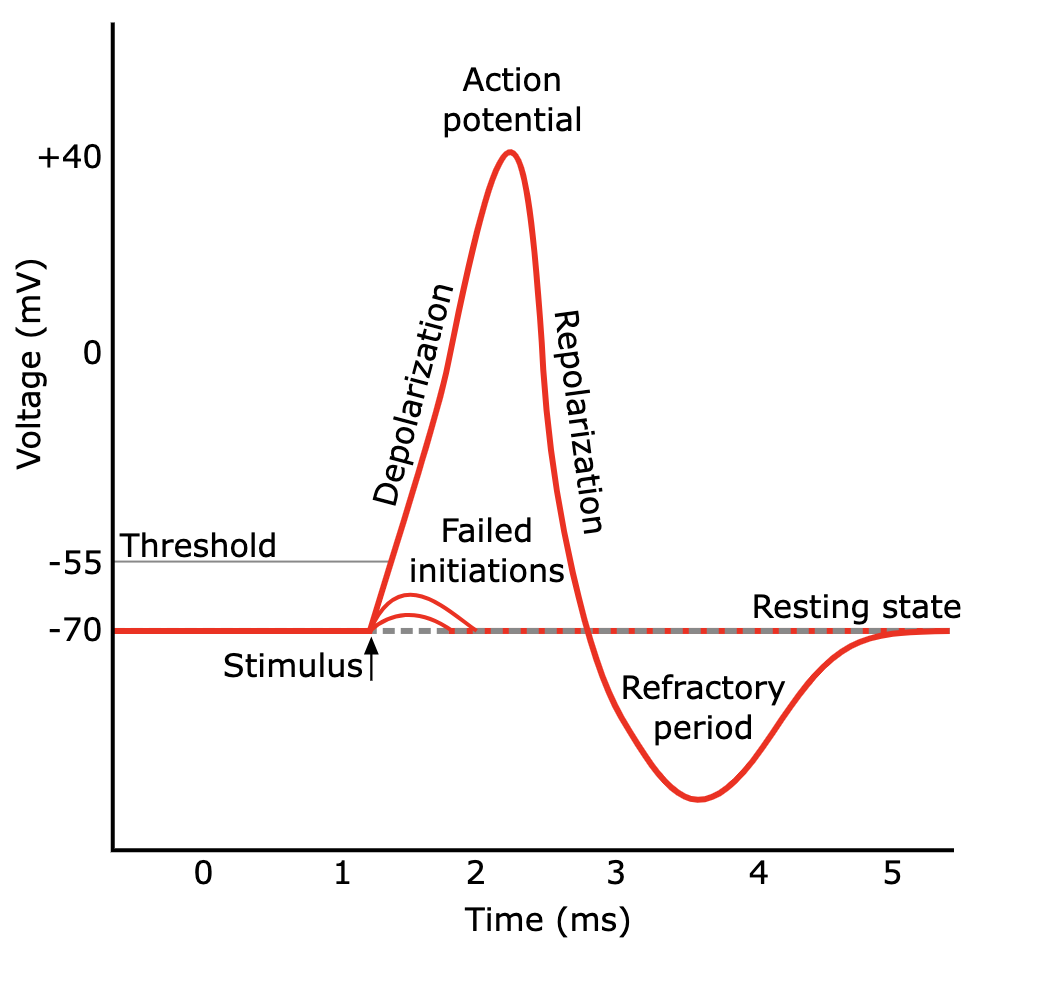
\includegraphics[width=0.8\linewidth]{figures/action_potential.png}
    \caption{Illustation of a characteristic action potential. The figure is taken from ... \rednote{Add proper figure text and citation}}
    \label{fig:action_potential}
\end{figure}

The action potential is characterised by a swift and steep rise in the electrical potential, resulting in a rapid upward, positive spike, followed by a quick decline in the potential back to the resting state. This form of the action potentials remains relatively constant throughout the propagation along the axon. When collecting information out of these spikes, it is therefor not the shape of the spikes that is studied. Instead, the information lies in the number and timing of chains of action potentials emmitted by the neuron, also reffered to as \emph{spike trais}.

Spike trains observed during epileptic seizures exhibit distinguishable characteristics compared to "normal" spike trains in regular neural activity. Epileptic seizures are characterized by regular, symmetrical, and generalized EEG patterns known as spike-and-wave discharges. These discharges result from bilateral synchronous firing of neurons within the thalamocortical network \cite{wiki:electroencephalography}. The spike-and-wave discharges manifest as a repetitive and rhythmic pattern, typically around 2.5 Hz or higher, setting them apart from the more irregular and unpredictable firing of action potentials seen in spike trains from healthy patients \cite{gerstner2014neuronal}. During epileptic events, the initiation of these discharges involves complex mechanisms, including the interplay of voltage-gated sodium and calcium channels and the role of inhibitory postsynaptic potentials \cite{wiki:electroencephalography}.
%This stark contrast in the rhythmicity and temporal dynamics of epileptic spike trains highlights the distinct nature of epileptic activity when compared to the more variable and less periodic patterns observed in "normal" neuronal firing \cite{gerstner2014neuronal}.

% Need to be rewritten somehow.
% The hypersynchronous discharges that occur during a seizure may begin in a very discrete region of cortex and then spread to neighboring regions. Seizure initiation is characterized by two concurrent events: 1) high-frequency bursts of action potentials, and 2) hypersynchronization of a neuronal population. The synchronized bursts from a sufficient number of neurons result in a so-called spike discharge on the EEG. At the level of single neurons, epileptiform activity consists of sustained neuronal depolarization resulting in a burst of action potentials, a plateau-like depolarization associated with completion of the action potential burst, and then a rapid repolarization followed by hyperpolarization. This sequence is called the paroxysmal depolarizing shift. (Slide 23) The bursting activity resulting from the relatively prolonged depolarization of the neuronal membrane is due to influx of extracellular Ca++, which leads to the opening of voltage-dependent Na+ channels, influx of Na+, and generation of repetitive action potentials. The subsequent hyperpolarizing afterpotential is mediated by GABA receptors and Cl− influx, or by K+ efflux, depending on the cell type.

% spike-and-vale / epileptiform activity  ... can be measured on eeg recordings... blabla .... spike trains looks like for epilepsy ... can be picked up on eeg recordings
% MAYBE NOT INCLUDE anything about eeg here, if anything, include how one can pick up on abnormal activity  ??

\section{Anatomy of the Cortex}
% Taken from the book and need to be rewritten !
Neurons in the brain are part of a vast network, interwoven with billions of other neurons and glial cells, creating the complex brain tissue. The brain is divided into various regions, and one essential area is the cortex, a thin but expansive sheet of neurons that folds over other brain structures. Different cortical areas have specific roles; some are specialized in processing sensory information, while others handle working memory or control motor functions \cite{gerstner2014neuronal}.

The human cerebral cortex consists of up to six layers of neurons. The oldest part of the cortex, known as the archipallium, has a more straightforward structure with three distinct neuronal layers. Within the archipallium, the hippocampus plays a major role in learning and memory functions. It is a crucial cortical structure implicated in the development of some common epilepsy syndromes \cite{bromfield2006introduction}.

Neurons communicate through synapses, where \emph{presynaptic neurons} sends, and \emph{postsynaptic cells} receives the information. In the animal brain, a single presynaptic neuron can connect to over 10,000 postsynaptic neurons. While many axonal branches end close to the neuron itself, some axons extend several centimeters to reach neurons in other brain regions \cite{gerstner2014neuronal}.

Within the cortex, there are two primary classes of neurons. Pyramidal neurons send information to distant areas of the brain, and they play a crucial role in long-distance communication. On the other hand, basket cells are considered local-circuit neurons, exerting their influence on nearby neurons. Most principal neurons form excitatory synapses, meaning they stimulate post-synaptic neurons, while most basket neurons form inhibitory synapses, meaning they suppress the activity of principal cells or other inhibitory neurons \cite{bromfield2006introduction}.


% \section{Head Models and Multicompartmental Modeling }
% % Something more about volume conducters
%
% \section{Currents and Potentials in the Brain}
% Ohm's law in volume conductors is a more genral statement than its usual form in electrical circuits. It is a linear relationship between vector current density $J$ and the electric field $E$. The law is then expessed as follows:
%
% \begin{equation}
% J = \sigma E,
% \label{eq:ohms_law}
% \end{equation}
%
% where $\sigma$ is the conductivity of the .... (physical material). (Soruce: Electric Fields of the Brain: The Neurophysics of EEG).
\end{document}

% eeg, head models etc
\documentclass[a4paper, UKenglish, 11pt]{uiomaster}
\usepackage{lipsum}
\usepackage[subpreambles=true]{standalone}


\begin{document}
\chapter{Electroencephalograpy}
Some words about what the background chapter will include.

\section{Neuroscience and Electroencephalography}
% Introduce neuroscience
% Nice words about EEG and how it works and is connected to neuroscience

Electroencephalography (EEG) is a non-invasively technique for studying electrical potentials in the human brain. The technique was developed almost a century ago making it among the oldest methods for examining the brain's activity. Today, EEG remains one of the most important techniques being used to study electrical activity in the brain, with important applications in both neuroscientific and clinical research (Nunez and Srinivasan 2006, Lopes da Silva 2013, Biasiucci et al. 2019, Ilmoniemi and Sarvas 2019).

EEG signal is believed to originate from large numbers of synaptic inputs to populations of geometrically aligned pyramidal neurons (Nunez and Srinivasan 2006, Pesaran et al. 2018).

Electroencephalography (EEG) is one of the most important techniques for studying cognition and disease in the brain non invasively. EEG is a method used to measure brain waves. In practice, this involves electrodes consisting of small metal disks connected to the surface of the scalp. The electrodes detect electrical charges that result from activity of the brain cells. In cases where certain areas of the brain come out as more active than others, it might indicate abnormalities, in which can be signs of disease. In other words, the EEG technique can be used to evaluate multiple types of brain disorders, such as lesions of the brain, Alzheimer's disease, epilepsy or brain tumors.

\begin{figure}
    \centering
    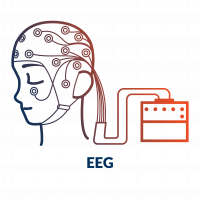
\includegraphics[width=\linewidth]{figures/EEG.png}
    \caption{Illustration of the EEG method.}
    \label{fig:EEG}
\end{figure}

An illustration of the typical EEG measurement setup is depicted in Figure \ref{fig:EEG}.

EEG signals are generated from synaptic inputs to cells in the cortex. Synaptic inputs are electrical (or chemical) signals that are being transmitted from one neuron to another, causing changes in the membrane potential of the neurons. In other words, neurons are specialized to pass signals, and synapses are the structures that make this transmission possible.

Imagining a small part of the cortex, all of these cells will have dendrites pointing upwards in the same direction (lets say the z-direction). Due to rotational symmetry around the z-axis, the contributions in the x- and y-direction will cancel. This is illustrated in Figure \ref{fig:EP}. What we see is that the extracellular potential is configured in all sorts of weird ways (A-C) when there is only one synaptic input, while the extracellular potential reminds more of a dipole when we have multiple synaptic inputs (D-F). We can therefore argue that the total contribution to the extracellular potential can be modelled as a dipole in the z -direction for the case where we have multiple synaptic inputs. Hence, for each dipole moment in our simulations, we assume multiple synaptic inputs, and make sure to rotate the positions of the dipoles such that it is orientated along the depth of the cortex.


\begin{figure}
    \centering
    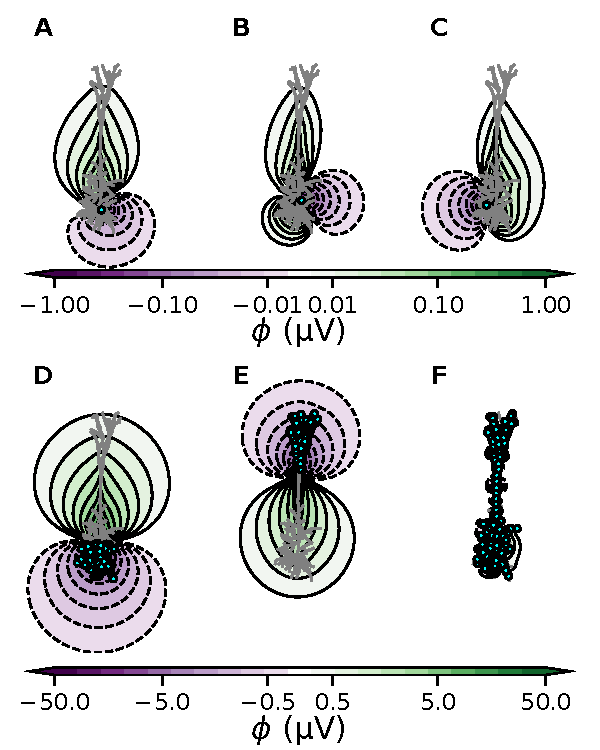
\includegraphics[width=\linewidth]{figures/fig_chosen_dipoles.pdf}
    \caption{Extracellular potential from lonely synaptic input (A-C) and extracellular potential from multiple synaptic inputs (D-F).}
    \label{fig:EP}
\end{figure}


\section{Currend Dipoles Approximation}
EEG signals arise from cortical neural activity and are typically described in terms of current dipoles.

An optimal model of EEG signals would have consisted of multiple dipole moments. However, as such a model is complicated and computationally expensive, we will in this project only introduce one single dipole approximation $\textbf{p}(t)$ for each multicompartmental neuron simulation. In this context, by  multicompartmental modelling we refer to the widely used models within neuroscience, which acurately manufactures electical properties of single neurons. The sigle-dipole approximation might sound like a substantial simplification of the real biophysical properties, nevertheless it actually turns out to give a realistic modelling of EEG signals, when handling the single dipole moment, as an abnormality in the brain. We will be thinking of the abnormality as an epileptic seizures or a tumor in the brain, which among normal activity in the brain would have stuck out. The single-dipole approximation is implemented by summing up the multiple current dipole moments,
\begin{equation}
    \textbf{p}(t) = \sum_{k=1}^M \textbf{p}_k(t) = \sum_{k=1}^M I_k^{\text{axial}}(t)\textbf{d}_k,
\end{equation}
where $I^{\text{axial}}$ is the current flowing along the neurite with the distance vector $\textbf{d}_k$ and $M$ denotes the number of axial currents. The data set we will be using in this project will consist of measures of different EEG signals at a given time from 1000 patients. This means that we for each patient pick a random location (at $t=0$) for the single current dipole.

\section{The New York Head Model}
The signals received from EEG are known to originate from cortical neural activity, which are often described by using current dipoles. It is therefor reasonable to implement current dipoles in the brain for when generating a biophysical modeling of EEG signals. The brain model used in this thesis is called the New York Head model, and is based on high-resolution anatomical MRI-data from 152 adult heads. The model utilizes the software tool LFPy, which is a Python module for calculation of extracellular potentials from multicompartment neuron models. This model takes into account that electrical potentials are effected by the geometries and conductivities of various parts of the head.

The cortex matrix consists of 74382 points, which refer to the number of possible positions of the dipole moment in the cortex. When generating our data set, we will for each sample randomly pick the position of the dipole moment, such that one sample corresponds to one patient. In our head model we are considering 231 electrodes uniformly distributed across the cortex, meaning that each EEG sample will consist of this many signals for each time step. However, we are not interested in the time evolution of the signals as this does not affect nor say anything about the position of the dipole moment, and we therefor simply pick out the EEG signals for when $t$ = 0 (note that the choice of time step could have been randomly picked). Our final design matrix will then consist of 1000 rows, corresponding to each patient, and 231 columns also refereed to as features, representing the signal of each electrode. The final output we are trying to predict is then the one dimensional vector with length 1000, where each element consists of the x-, y- and z- position of the dipole moment. An example of how the input EEG signals may look like is given in appendix A, where we also have marked the dipole moment with a yellow star.

\section{The Inverse Problem and Source Localization}

% To solve the inverse EEG problem, various algorithms and methods have been developed, such as Minimum Norm Estimates (MNE), Low Resolution Electromagnetic Tomography (LORETA), and Dynamic Imaging of Coherent Sources (DICS). MACHINE LEARNIG....

% The inverse EEG problem is the problem of determining the sources of electrical activity within the brain that give rise to the measured EEG signal. The EEG signal is a recording of the electrical activity of the brain, which is measured at the surface of the scalp. However, the electrical activity that gives rise to the EEG signal is generated by a large number of sources within the brain, and it is not possible to determine the location or number of these sources just by looking at the EEG signal alone. Therefore, the inverse EEG problem is the problem of determining the sources of the EEG signal based on the measurement of the signal itself.

% To solve the inverse EEG problem, various algorithms and methods have been developed, such as Minimum Norm Estimates (MNE), Low Resolution Electromagnetic Tomography (LORETA), and Dynamic Imaging of Coherent Sources (DICS).

% However, the problem remains very challenging, as the EEG signal measured at the scalp is the result of a complex and unknown combination of sources, the brain anatomy itself and the volume conductor contribute to the complexity of the problem.

% As of now, there is not yet a definitive solution for the Inverse EEG problem and the area is still active research topic.

\end{document}

% machine learning and NN
% !TEX root = main.tex
\documentclass[a4paper, UKenglish, 11pt]{uiomaster}
\usepackage{lipsum}
\usepackage[subpreambles=true]{standalone}
\usepackage{graphicx}

\begin{document}

\chapter{Method: Creating EEG Data} \label{chap:eeg_data}
In preparation for the application of neural networks to address the inverse problem, the acquisition of an appropriate EEG data set is essential. This chapter focuses on utilizing the New York Head model in conjunction with the current dipole approximation to construct biophysically realistic EEG data.
In Section \ref{chap:simulation}, we will provide a detailed exploration of our EEG data simulation methods. Moving forward to Section \label{chap:noise}, we will discuss the introduction of noise and its significance. Section \ref{chap:final_data} summarizes the features of the final data set, which will be used to train models for solving the EEG inverse problem.


\section{Simulation of EEG Signals from Single Dipoles} \label{chap:simulation}
% The New York Head model and its  were made available for reuse in the {\tt h5py} Python package.
To create EEG data we use the New York Head model and its lead field matrix, which are integrated into the Python module LFPy 2.0 \cite{LFPy}. This software is a userfriendly wrapper around the NYHM, allowing for simulations of neural activity and the resulting EEG signals. Within LFPy, we use the \texttt{NYHeadModel} class to calculate EEG signals originating from a desired current dipole moment. For more information about the LFPy module, we refer the reader to Hagen, Næss, Ness and Einevoll (2018) \cite{LFPy}.

The implementation of the lead field matrix in the \texttt{NYHeadModel} class in LFPy consists of 74,382 discrete points, each representing potential dipole source locations within the cortex. To sample a single data point we position a current dipole moment at one of the possible locations, and calulate its corresponding EEG signal according to the procedure outlined in Chapter \ref{chap:eeg}. To begin with, we maintain uniform magnitudes for the dipole signals. By setting these magnitudes to 1 nAm, the resulting EEG measurements span a range of approximately -1 to 1 $\mu$V. The NYHM is solved for 231 electrode possitions. One sample consequently holds the signal measured at each of the 231 electrodes at the scalp.

To ensure that the dipole orientations are predominantly aligned with the radial direction of the cortex, as emphasized in Chapter \ref{chap:eeg}, each dipole moment is rotated to be normal to the surface of the cerebral cortex. Note that aligning the dipole orientations radially to the cortex does not always lead to the dipole's normal vector pointing directly outward toward an EEG electrode. This variability arises due to the complex folding patterns found in the human cortex. In certain cases, when a dipole is located within a sulcus, the electrical signal it generates originates deep in the brain. Consequently, the electrical signal must traverse a longer path before reaching an EEG electrode \cite{naess2021biophysically}.

In the preceding chapter, we discussed how EEG analysis often revolves around the exploration of specific frequency bands. However, an alternative and widely recognized method for EEG investigation involves the practice of averaging EEG responses to specific stimuli across multiple trials \cite{kropotov2016functional}. These temporally aligned segments of EEG signals are commonly referred to as event-related potentials (ERPs). Given that noise and various EEG components are assumed to exhibit random variations across samples, the averaging procedure effectively reduces noise and extracts the event-related activity. In other words, this technique facilitates the identification of the specific time step within the EEG time series where the averaged signal attains its maximum magnitude, resulting in a 'static' EEG signal characterized by reduced noise.

The underlying principle for this approach is the quasi-static approximation, which posits that the potential measured from a dipole propagates instantaneously from the source to the electrode. This simplification is based on the assumption that the EEG signal at any point effectively captures a snapshot of the dipole activity within the brain. This means that if a dipole exhibits oscillations at a particular frequency, the corresponding EEG signal will oscillate at the same frequency, without phase shifts \cite{plonsey1967considerations}.

In our analysis, we sample the EEG data to obtain what we may consider an ERP, effectively representing a static snapshot of the electrode recordings of a current dipole source with magnitude 1 nAm. This alternative to the traditional time series data offers simplification and computational efficiency without significant deviation from standard clinical EEG analysis. This construction is further justified by the fact that our simulated data is noise-free, eliminating the risk of noise interference with the EEG samples. Consequenscly, we are left with time-locked, one-dimensional EEG signals mirroring the electrode recordings of dipoles located at different positioning within the cerebral cortex.

In our data collection, we sample the EEG data to obtain what we may consider an ERP, effectively representing a static snapshot of the electrode recordings of a current dipole source with a magnitude of 1 nAm. In contrast to clinical analyses of ERPs, we simulate one event per sample and do not hesitate to average over multiple events to collect the final signal. This approach is justified by the fact that our simulated data is noise-free, eliminating the risk of noise interference with the EEG samples. This simulated ERP data can be viewed as an alternative to traditional time series data, offering simplification and computational efficiency without significant deviation from standard clinical EEG sampling. Consequently, we are left with time-locked, one-dimensional EEG signals mirroring the electrode recordings of electrical potentials generated by dipoles located at various positions within the cerebral cortex.


\section{Noise} \label{chap:noise}
Real-world EEG recordings inevitably contain noise, which can disrupt the accurate analysis of brain activity. \emph{Artifacts}, which are signals recorded by EEG but originating from sources other than neuronal communication, pose a particular challenge in real-world data. Some artifacts can mimic genuine epileptiform abnormalities or seizures, underscoring the importance of identifying and distinguishing them from true brain waves \cite{sazgar2019eeg}.

Artifacts can be classified into two categories based on their origin. \emph{Physiological artifacts} arise from the patient's own physiological processes, including ocular activity, muscle activity, cardiac activity, perspiration, and respiration. \emph{Technical artifacts}, on the other hand, are electromagnetic interferences from external factors such as cable and body movements \cite{bitbrain}.

Filtering techniques are commonly employed to mitigate artifacts in EEG recordings before conducting analyses. It is important to note that while these techniques can significantly reduce noise, they may not completely eliminate all sources of interference. In the context of simulated EEG data, there is no inherent noise present. However, to align the simulated data with real-world EEG samples, controlled noise is intentionally introduced. This process ensures that the simulated EEG data closely resembles real measurements that have undergone appropriate filtering and preprocessing. Consequently, the data maintains a high signal-to-noise ratio (SNR) while incorporating a realistic amount of noise disturbance.

Utilizing realistic data is a critical step in enhancing the robustness of the trained neural network, thereby ensuring its effectiveness in handling real EEG recordings. However, the specific characteristics and quantity of noise have not been the primary focus of our study, and we have therefore adopted a straightforward approach in our methodology. Our final data set incorporates normally distributed noise with a mean of 0 and a standard deviation equal to 10$\%$ of the standard deviation observed in the simulated EEG recordings. This introduced noise introduces random variations around each data point, all while preserving the overall statistical properties of the data set.


\begin{figure}[!htb]
    \centering
    \hspace*{-3cm}
    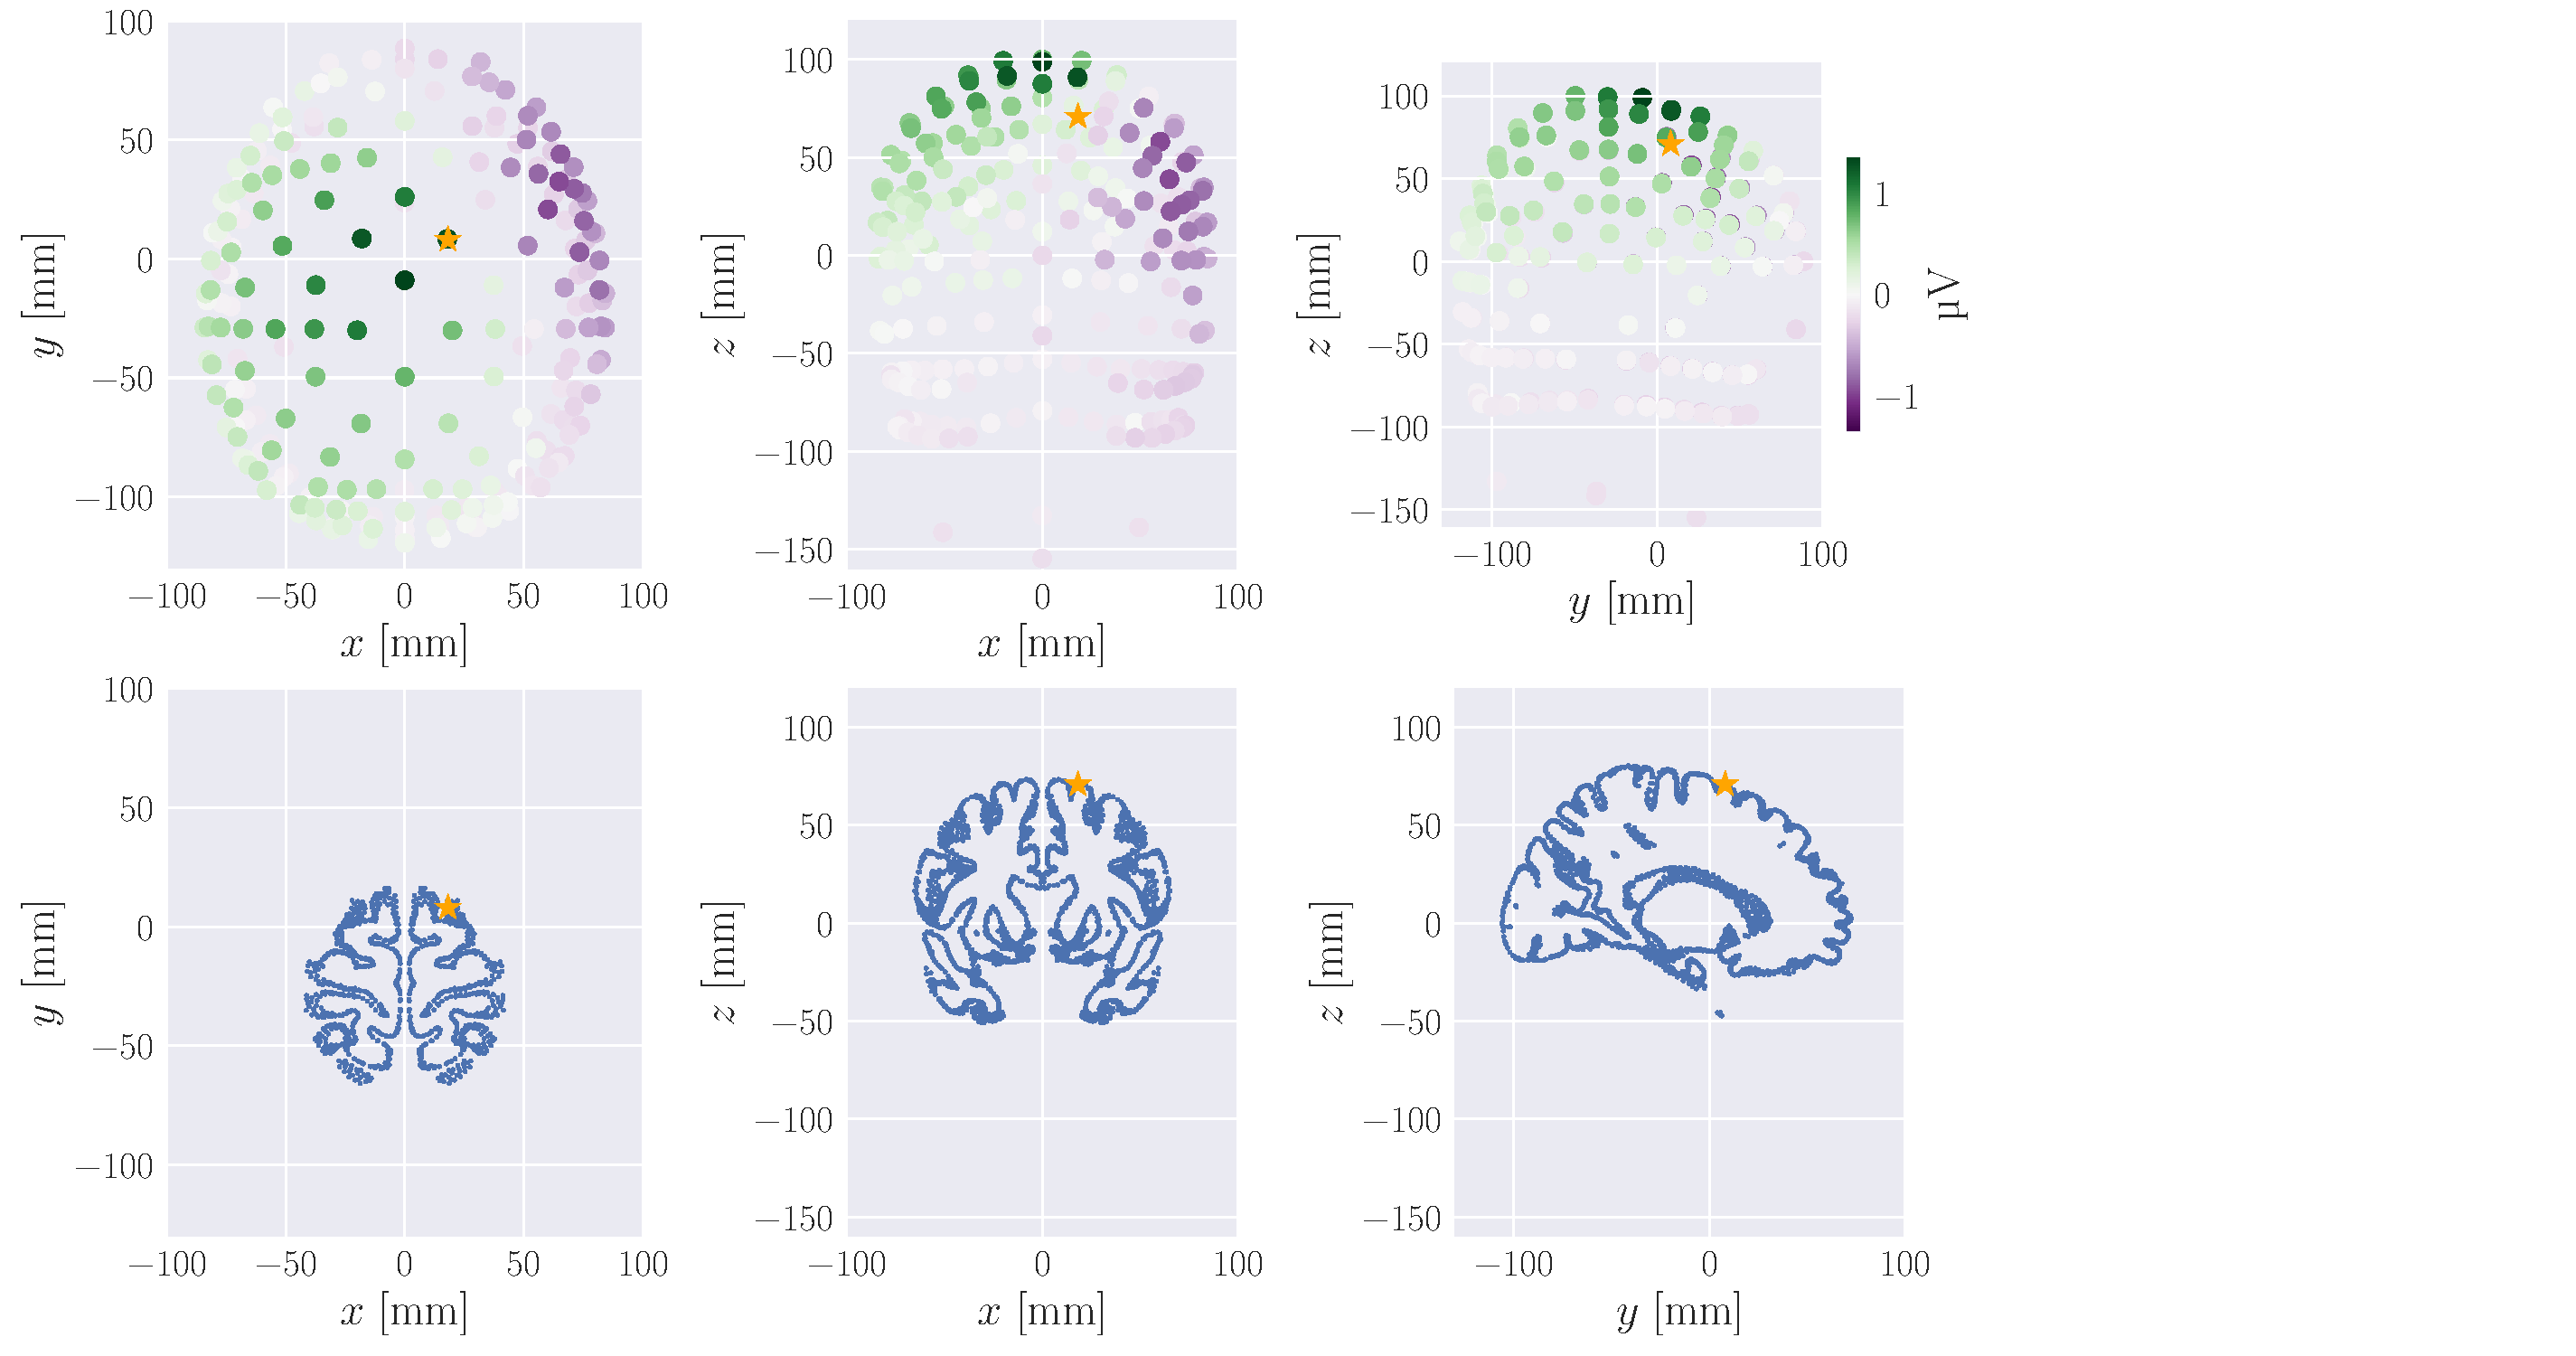
\includegraphics[width=18cm]{figures/purple_green/simple_example.pdf}
    \caption{EEG measurements for a sample containing one single current dipole source at an arbitrary position within the celebral cortex. Noise is added to the EEG signal. The EEG measure is seen from both sides ($xz$-plane and $yz$-plane) and above (the $xy$-plane). EEG electrode locations are presented as filled circles, where the color of the fill represents the magnitude of the measured signal for the given electrode. The position of the current dipole moment is marked with a yellow star.}
    \label{fig:eeg_field_1_dipole_example}
\end{figure}


\section{Final Dataset} \label{chap:final_data}
\rednote{Remove?}
The final data set, $\mathcal{D}$, comprises 70,000 samples, where each sample holds 231 values representing the EEG measurements recorded at each electrode -- a configuration directly inherited from the NYHM. Target values for the EEG samples are the $x$-, $y$- and $z$-coordinates of the different dipole sources.

Figure \ref{fig:eeg_field_1_dipole_example} presents an example of the input EEG data for a single sample, with added noise. The prominent dipolar pattern in the figure indicates that the dipole is located within a sulcus. In the figure the EEG measure is visualized from multiple perspectives: the $xz$-plane, $yz$-plane, and the $xy$-plane. The electrode locations are represented by filled circles, with the color of the fill indicating the magnitude of the measured signal at each electrode. The position of the current dipole moment is denoted by a yellow star. As indicated by the colorbar in the figure, the EEG signal for the specific sample ranges from -1 to 1 $\mu$V, which is the range that the simulated EEG data for all samples will fall within.



% Before being feed to the DiLoc network for training, the data is splitted into train, validation and test parts. The train- and validation data are the batches of the data set that the network uses during training. Out of the 70 000 samples in the final dateset, 50000 is set off to the purpose of train and validation data. Out of these 50000 sampes, randomly selected 80 percent of the rows are put into the training set. The remaining 20 percent operates as the validation set, which is useful in order to prevent the network to overfit during training. The test set which contains the final 20 000 samples will be used after the training prosess for the purpose of testing how well the model generalizes to new, unseen data.
%
% Prior to being fed into the DiLoc network for training, the data set was splittied into distinct segments: the train, validation, and test sets. This partitioning is vital for assessing and optimizing the network's performance. Among the 70 000 samples in the final data set, 50 000 samples are designated for the train and validation data. To ensure a representative and unbiased allocation, 80 percent of these 50 000 samples are randomly assigned to the training set. This training set serves as the core data that the network utilizes during the training process. The remaining 20 percent of the 50 000 samples form the validation set. This set plays the role in preventing overfitting, the phenomenon where the network becomes excessively attuned to the training data and consequently performs poorly on new data. By independently evaluating the model's performance on the validation set throughout training, we can fine-tune the network's parameters to achieve better generalization to unseen data. Once the network completes its training process, the test set comes into play. Comprising 20 000 samples, the test set serves as the benchmark for assessing the model's ability to generalize and make accurate predictions on new data instances. By adhering to this rigorous train-validation-test data partitioning, we ensure a robust evaluation of the DiLoc model's performance and its capacity to effectively handle real-world scenarios with previously unseen data.



\end{document}


% methods in ML (?)
% !TEX root = main.tex
\documentclass[a4paper, UKenglish, 11pt]{uiomaster}
\usepackage{lipsum}
\usepackage[subpreambles=true]{standalone}
\usepackage{graphicx}

\begin{document}


\chapter{A Fully Connected Feed-Forward Neural Network Approach to Source Localization} \label{chap:fcnn-approach}
\chaptermark{FCNN Approach}

Having obtained a suitable data set we can start building neural networks to address the EEG inverse problem. In this chapter, we provide a comprehensive overview of a feed-forward neural network built to map measured EEG signals to corresponding locations of current dipoles. We will be discussing its architecture and parameters.\rednote{Introduce what the sections will be about.}

\section{Machine Learning}
\rednote{cite!!!!}
The field of machine learning is concerned with constructing computer programs that learn from experience. Within this computational discipline we find a spectrum of tasks these algorithms aim to understand and accomplish. For the purpose of solving the EEG inverse problem the model is concerned with the task of localizing the origins of abnormal electrical brain signals within the human cortex. The machine learning algorithm will gain experience through the analysis of corresponding EEG data associated with these abnormal sources.

Typically, machine learning problems are addressed using the same three elements.
The first element is the data set $\mathcal{D} = (X, Y)$. $X$ is commonly referred to as the \emph{design matrix} and $Y$ is the set of \emph{target values} we want the model to predict as function of the elements in $X$.
Next, we have the model $f(x; \boldsymbol{\theta})$ itself which is a function $f : \mathcal{X} \to \mathcal{Y}$ used to predict an output $y \in \mathcal{Y}$ from an input $x \in \mathcal{X}$ using the \emph{model parameters} $\boldsymbol{\theta}$.
Thirdly we have the cost function $C(y, f(x; \boldsymbol{\theta}))$ for $x \in \mathcal{X}$ and $y \in \mathcal{Y}$, which allows us to evaluate how well the model performs on the samples in $\mathcal{D}$. Training a machine learning model involves the adjustment of the model parameters $\boldsymbol{\theta}$ to minimize the cost function. The cost function yields high values when the model's output deviates from the desired target, and conversely, it produces smaller values when the predictions align closely with the intended outcomes. The output of the cost function is commonly referred to as the model's \emph{cost} or \emph{loss}. We will be using these terms interchangeably.





\section{Neural Networks}

Neural networks are a distinct class of so-called \emph{nonlinear machine learning models} capable of learning tasks by observing examples, without requiring explicit task-specific rules \cite{Hjorth-Jensen2022}. The models mimic the way biological neurons transmit signals, with interconnected \emph{nodes} that communicate through mathematical functions. Each connection between nodes is represented by a \emph{weight} variable, which encodes the strength of the communication between the two nodes. During training, the neural network ``learns'' by adjusting these weights to capture the underlying patterns and relationships in the data.

We will mainly consider fully connected feed-forward neural networks, henceforth abbreviated as FCNNs, whose nodes are grouped into \emph{layers} with the output of one layer serving as the input for the next. Typically, we call the first layer of neural networks the \emph{input layer}, the final layer of the model \emph{output layer} and the layers in between \emph{hidden layers}. What lies in the term ``fully connected feed-forward'' is that every node within each layer sends their outputs to every node the next layer. Generally speaking, the outputs is only sent forward, through all of the layers.
The activation $a_i^{(l)}$ of the $i$-th node in layer $l$ is the weighted sum
\begin{equation}
  z_i^{(l)} = \sum_{j=1}^{N_{l-1}} w_{ij}^{(l)} a_{j}^{(l-1)} + b_i^{(l)}
  \label{activation_node}
\end{equation}
fed through an \emph{activation function} \(\text{act}\):
\begin{equation}
  a_i^{(l)} = \text{act} \left( z_i^{(l)} \right).
\end{equation}
$N_{l}$ is the number of nodes in layer \(l\).
Activation functions introduce nonlinearity into the network's computations. They play a critical role in enabling the model to capture nonlinear patterns within the data. The \emph{bias} \(b_i^{(l)}\) and the weights \(w_{ij}^{(l)}\) are the trainable parameters \(\boldsymbol \theta\) of the model.


% In figure \ref{fig:NN_basic_architecture} we have illustrated the basic architecture of neural networks. Here nodes are depiced as circular shapes, while arrows indicate connections between the nodes. \rednote{maybe remove first figure? wrong notation}.

% \begin{figure}
%     \centering
%     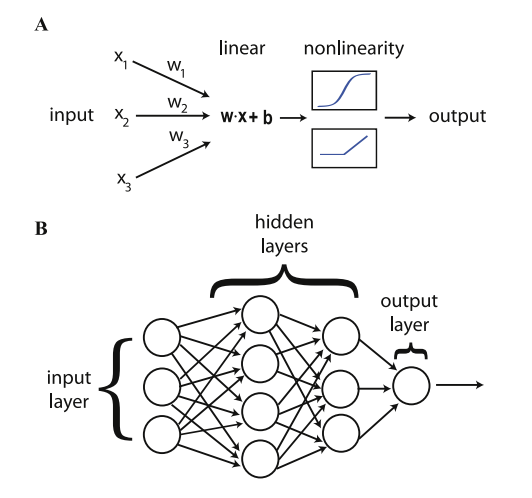
\includegraphics[width=10cm]{figures/basic_architecture.png}
%     \caption{$\textbf{(A)}$ The fundamental structure of neural networks comprises simplified nodes units that perform a linear operation to assign different weights to inputs, followed by a nonlinear activation function. $\textbf{(B)}$ These nodes units are organized into layers, where the output of one layer serves as the input to the subsequent layer, forming a hierarchical arrangement. \rednote{Add proper citation.}}
%     \label{fig:NN_basic_architecture}
% \end{figure}



% where $a$ is the output of the node, and is the value of the nodes activation function $f$ which has as input a weighted sum of signals $x_i, x_{i+1},...,x_n$ recieved by $n$ other nodes, multiplied with the weights $w_i, w_{i+1}, ..., w_{n}$ and added with biases $b_i, b_{i+1}, ..., b_{n}$. Biases, represented by $b_i$ for each node, provide an additional adjustment to the weighted sum, allowing the network to model biases in the data and play a crucial role in the overall flexibility of artificial neurons. The exact expression of $a$ varies depending on the type of nonlinearity that exists in the activation function applied to the input of each node. However, in almost all cases $a$ can be decomposed into a linear operation that weights the relative importance of the various inputs, and a nonlinear transformation $f(z)$. As seen in equation \ref{eq:neuron}, the linear tranformation commonly takes the form of a dot product with a set of node-specific weights followed by re-centering with a node-specific bias. A more convenient notation for the linear transformation $z^{i}$ then goes as follows:
%
% \begin{equation}
% z^{i} = \boldsymbol{w}^{(i)} \cdot \boldsymbol{x} + b^{(i)} = \mathbf{x}^T \cdot \mathbf{w}^{(i)} ,
% \label{eq:linear_transformation}
% \end{equation}
%
% where $\mathbf{x} = (1, \boldsymbol{x})$ and $\mathbf{w}^i = (b^{(i)}), \boldsymbol{w}^{(i)})$. The full input-output function can be expressed by incorporating this into the nonlinear activation function $f_i$, as expressed below:
% % TODO: f_i or a_i here?
%
% \begin{equation}
% a_i(\mathbf{x}) = f_i(z^{(i)}) .
% \label{eq:linear_transformation}
% \end{equation}


\section{Building a Feed-Forward Neural Network}
%The development of DiLoc started with a deliberate and cautious approach, focusing on simplicity without compromising on accuracy in tackling the inverse problem.
\rednote{Did not test other architectures?}
The feed-forward neural network was one of the first artificial neural network to be adopted and is yet today a wildly used algorithm within the domain of machine learning. As a natural starting point, we therefore adopted a fully connected, feed-forward neural network architecture for the purpose of solving the inverse problem. This approach eventually proved to be the most suitable framework among the ones tested. The fully connected feed-forward neural network is known as one of the simpler forms of neural networks, where information is processed in a unidirectional manner, flowing from the input nodes through the hidden layers and ultimately to the output nodes.



\subsection{Architecture}

% All inner parameters of the networks (weights and biases) are adjustable. Due to the layered structure of FNN the learning process is complicated, inefficient, and requires the activation functions of neurons to be differentiable. The training usually employ some form of gradient descent method, which is generally time-consuming and converges to local minima. Moreover some parameters, such as number of hidden neurons or learning algorithm parameters, have to be tuned manually.
% https://link.springer.com/chapter/10.1007/978-3-319-26227-7_6

In our initial testing phase, we tried different network configurations through an
iterative trial-and-error procedure. Different network architectures with various numbers of hidden layers and nodes were systematically examined. Ultimately, we settled on a model with roughly 300,000 trainable parameters which, after tweaking additional network attributes which will be elaborated upon later in this chapter, yielded promising results in terms of prediction accuracies.

The input layer is designed with 231 nodes, corresponding to the number of features in our data set, i.e. the number of recording electrodes for each sample. Subsequently, the network consists of five hidden layers, comprising 512, 256, 128, 64, and 32 nodes, respectively. Finally, the output layer holds an $x$-, $y$- and $z$-coordinate representing the predicted position of the dipole source. Figure \ref{fig:FCNN_architecture} visualizes the structure of the fully connected neural network.

\begin{figure}[!htb]
    \centering
    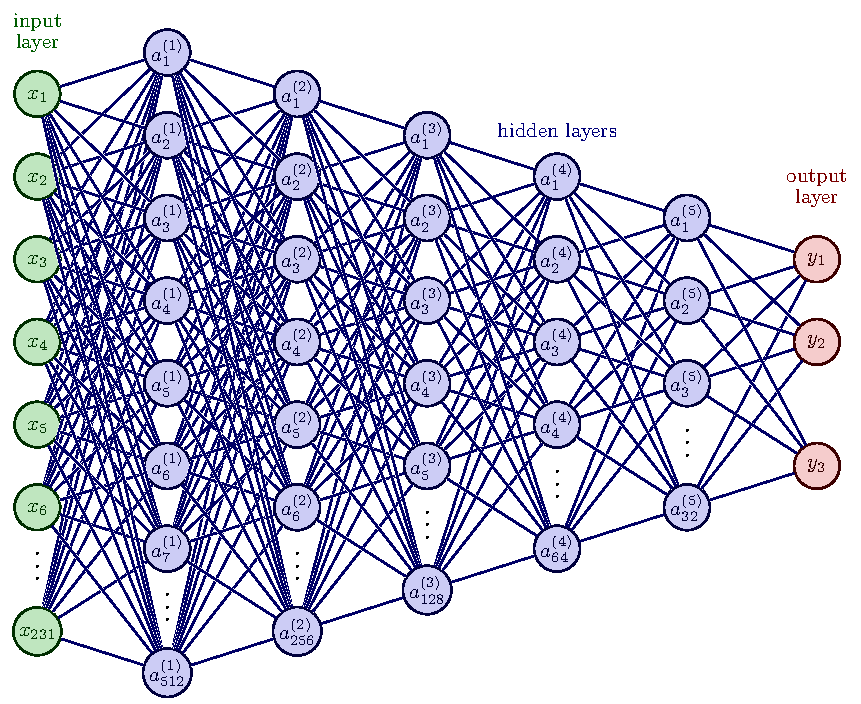
\includegraphics[width=\linewidth]{figures/FFNN_architecture.pdf}
    \caption{\textbf{Architecture of the fully connected Feed-Forward Neural Network}. The input layer comprises 231 electrode recording input values, and the network outputs predicted $x$-, $y$-, and $z$-coordinates of the dipole generating the EEG signal. The FCNN consists of five hidden layers. \\
    The visualization has been made with Latex, with code adapted from Neural Networks in TikZ with attribution to Izaak Neutelings and is licensed under the Creative Commons Attribution-ShareAlike 4.0 International License \cite{neutelings2021}.}
    \label{fig:FCNN_architecture}
\end{figure}



\subsection{Activation Functions}

Activation functions are fundamental components within the architecture of neural networks. Essentially, these functions introduce nonlinearity into the network's computations, thereby enabling the network to capture and model complex relationships within data \cite{sharma2017activation}. This property is essential because many real-world phenomena and data patterns exhibit inherent nonlinearity. Without activation functions, neural networks would essentially be linear regression models, limiting their ability to predict other relationships between inputs and outputs. In neural networks, activation functions are typically applied at every node within the hidden layers and sometimes at the output nodes in the final layer.
%In the context of solving the EEG inverse problem, where the EEG data contains intricate, nonlinear patterns, activation functions empower DiLoc to effectively model and learn from the EEG data structures.

Drawing inspiration from the behavior of biological neurons, activation functions can be understood as decision-makers within the artificial neural network, determining which information should be relayed to the next node. This process is analogous to the process in biophysics where the axon of one cell takes the output signal from the preceding cell and converts it into a format suitable for input to the next cell. Some activation functions can also be directly associated with biological phenomena like action potentials and spikes within neurons. Similar to how real neurons respond to incoming electrical signals, activation functions decide whether a node in a neural network should be activated or not based on the strength of the input it receives. If the input exceeds a certain threshold, the artificial neuron ``fires''; otherwise, it remains inactive \cite{analyticsvidhya_activationfunctions}.


\subsubsection{Rectified Linear Unit}
Within the input layer of the FCNN network, nodes utilize the \emph{Rectified Linear Units} (ReLU) activation function
defined as
\begin{equation}
  \text{ReLU}(x) = \begin{cases}
  x, & \text{if } x > 0 \\
  0, & \text{otherwise,}
\end{cases}
\label{eq:ReLU}
\end{equation}
and visually depicted in Figure \ref{fig:ReLU}.
ReLU closely resembles the behavior  of biological neurons. Specifically, it echoes the concept of the action potential: if a threshold is reached, the neuron fires; otherwise, the neuron remains inactive. Positive input values remain unchanged, while negative input values are suppressed by setting them to zero.
The widespread adoption of ReLU in neural networks can be attributed to its advantages in terms of computational speed, performance, and generalization capabilities.
\begin{figure}[ht]
    \centering
    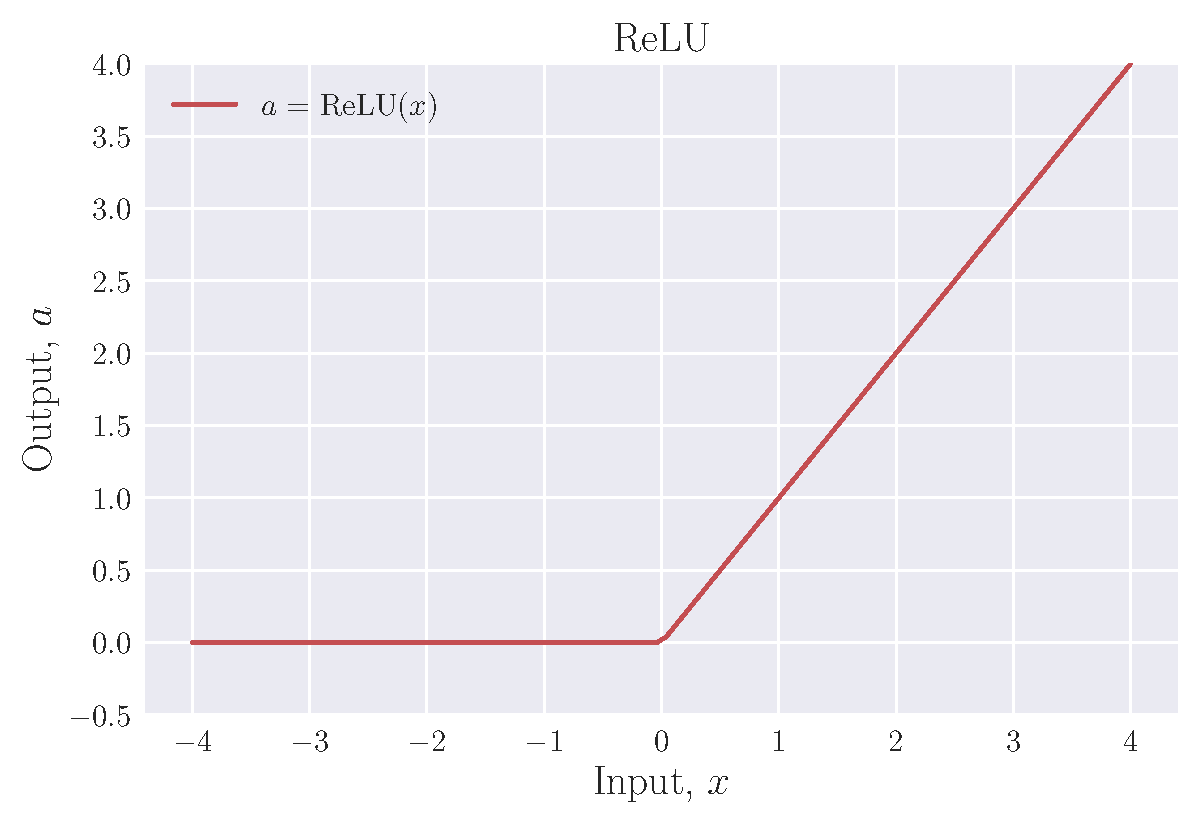
\includegraphics[width=\linewidth]{figures/ReLU.pdf}
    \caption{\textbf{Rectified Linear Unit (ReLU) Activation Function}: preserves positive input values \(x\) unchanged and enforces a transformation of negative input values to zero.}
    \label{fig:ReLU}
\end{figure}


\subsubsection{Hyperbolic Tangent}
For the hidden layers, we employed another activation function known as the \emph{Hyperbolic Tangent} (tanh) defined by
\begin{equation}
  \tanh(x) = \frac{e^x - e^{-x}}{e^x + e^{-x}},
\end{equation}
which is visualized in Figure \ref{fig:Tanh}.
This activation function smoothly compresses input values into the range between \(-1\) and 1, thereby preventing activations from becoming large, which could potentially cause problems during training.
While ReLU is known for its computational speed and simplicity, tanh has the possible advantage that it keeps all data flowing through the network during a forward pass. ReLU effectively removes the flow of information from some nodes through the network by clipping all negative values to zero. This could be a positive feature, but potentially also a problem causing some of the nodes to never be able to influence the output of the model, thereby decreasing its ability to learn.
\begin{figure}[ht]
    \centering
    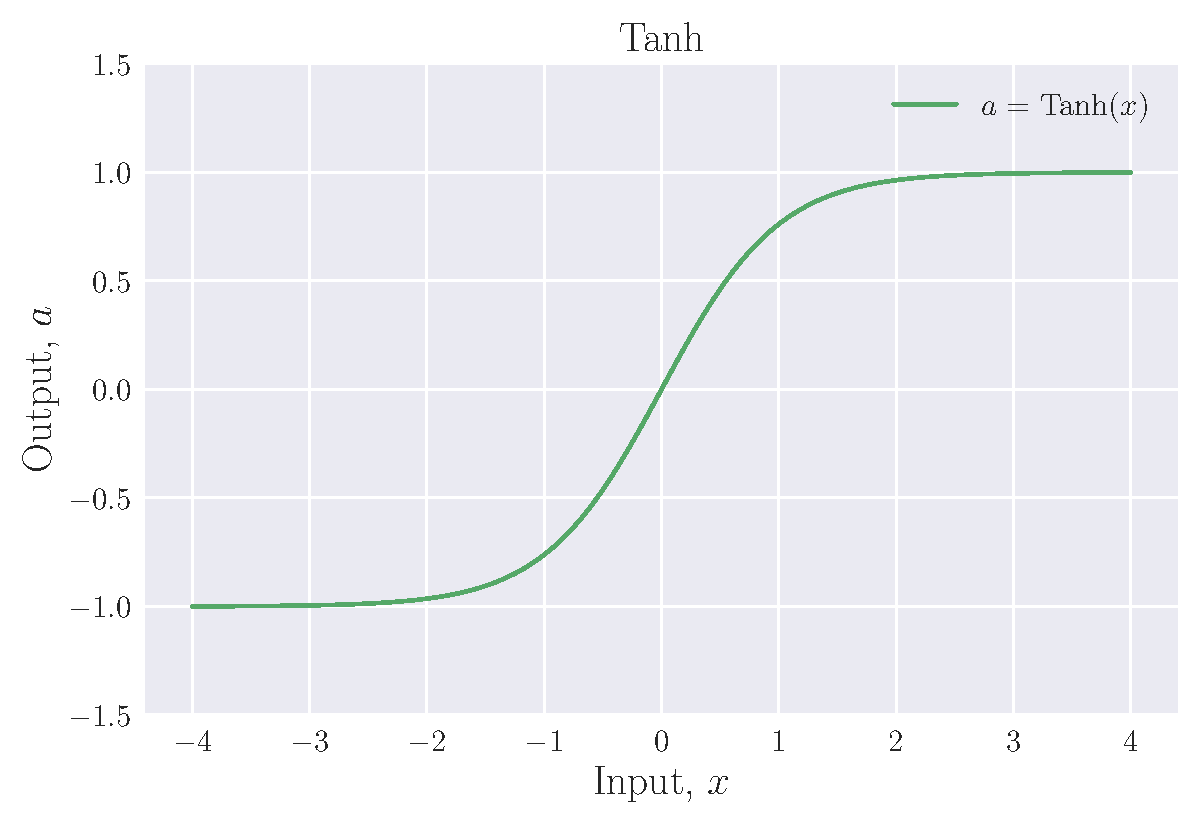
\includegraphics[width=\linewidth]{figures/Tanh.pdf}
    \caption{\textbf{Hyperbolic tangent activation function}: maps the input value $x$ into a continuous range between -1 and 1.}
    \label{fig:Tanh}
\end{figure}

%aim for the network to achieve a stable and effective learning process.
% tanh is continuous and differentiable at all points, that for reasons we will come back to is making it a suitable activation function for neural networks \rednote{Where do I come back to this?}.


\subsubsection{Linear Activation}

In our specific application, the target positions are the coordinates of current dipole sources, with values ranging from -70 to 70 mm for $x$, -58 to 78 mm for $y$, and -69 to 59 mm for $z$.
In the context of regression problems like ours, it is common practice to use linear activations -- which is simply the absence of any activation function at all -- in the output layer. We have done the same in our model, thus enabling it to output unbounded coordinate values.



\subsection{Initialization of Parameters}

% 231*512 + 512*256 + 256*128 + 128*64 + 64*32 + 32*3 + (512 + 256 + 128 + 64 + 32 + 3) = 293443

Neural networks train by fine-tuning their parameters \(\boldsymbol \theta\) to capture and adapt to intricate patterns within data. Weights and biases serve as the inner parameters of neural networks. The total number of parameters is equal to the sum of all connections between layers plus the total number of biases in every layer. In the architecture provided in Figure \ref{fig:FCNN_architecture}, our FCNN comprises just under 300,000 parameters.

The \emph{initialization} of weights and biases can significantly impact how quickly the model converges during training, and there exist several procedures commonly employed. In the FCNN we have used Xavier initialization, as this procedure is commonly paired with the tanh activation function, which is the one applied in our hidden layers. For every layer $l$, the weights $w^{(l)}$ are sampled from a normal distribution with mean \(\mu\) and variance \(\sigma^2\):
\begin{equation}
  w^{(l)} \sim \mathcal{N} \left( \mu=0, \sigma^2 = \frac{2}{N_{l-1} + N_l} \right).
\end{equation}
\(N_l\) denotes the number of neurons in layer \(l\).
\(N_l\) and \(N_{l - 1}\) are the number of rows and columns in \(w^{(l)}\) respectively.
The biases \(b^{(l)}\) are sampled uniformly between
\(- \sqrt{\frac{1}{N_{l - 1}}}\)
and
\(\sqrt{\frac{1}{N_{l - 1}}}\):
\begin{equation}
  b^{(l)} = \mathcal U \left( - \sqrt{\frac{1}{N_{l - 1}}}, \sqrt{\frac{1}{N_{l - 1}}} \right).
\end{equation}





\end{document}


%DiLoc network
\documentclass[a4paper, UKenglish, 11pt]{uiomaster}
\usepackage{lipsum}
\usepackage[subpreambles=true]{standalone}

% Explain EEG
% Explain how EEG sources can be modeled/simulated (include the first attempt done in 1949)
% Head models (New York Head Model)
% Maybe there should be an implementartion section ?

\begin{document}
\chapter{Results}
As mentioned in chapter 1, an important topic in EEG signal analysis is the inverse problem of going from measured EEG signals to localized equivalent current dipoles, so-called source localization. In this chapter we will present the training and performance of the neural networks presented in chapter 4. Section ... and ... deal with training of the simple feed forward neural network and presenting its results, while section ... will discuss how a convolution neural network can be used to obtain the same results. But first, we will take a look at the dataset being feed to the different networks.

\section{Simulation of EEG Signals}
The cortex matrix of the New York Head Model (NYHM) consists of 74382 points, which refer to the number of possible positions for localization of dipole sources. We will train the neural networks using a dataset of self-simulated EEG measurements that correspond to the electromagnetic fields generated by dipole sources. These sources will have randomly selected positions within the cortex matrix. However, to simplify the problem, the stengths of single dipoles (amplitude) are set to $10^7$ nA $\mu$ m. Moreover, in the cases of single dipole source localization, the direction of the dipole moment is always rotated so that it is normal to the cerebral cortex. In some cases this will result in a dipole moment pointing perpendicular to the skull (directed towards an EEG electorde), while in other cases, due to the structure of the cortex, the dipole moment will point back into the cortex (but eventually towards an EEG electorde). The reason for this is that the human cortex is strongly folded, and the contribution to the EEG signal from a neural population (dipole moment) will depend on whether a dipole is located in a sulcus or a gyrus (source: BookTVN).
\\
\\

\subsection{Effect of dipole location and orientation on EEG signals}
%The orientation of the cortical surface at a given location will, because of the sulci and gyri, affect how the local current dipoles will contribute to the EEG signal.
As shown by/ discussed in .... (source: BookTVN) EEG signals are relatively insensitive to small changes in the \emph{location} of neural current dipoles. Even though the intuitive thought might be that neurons in the upper cortical layers dominate the EEG due to the closer distance to the EEG electrode compared to neurons in the lower cortical layers, such differences in location acutually does not make conciderable differences. This finding can be explained by fact that the low conductivity of the skull generates a certain spatial low-pass filtering, that .... .
% Maybe what is meant here is that we therefore only consider the outer corical surface

\begin{figure}[!htb]
    \centering
    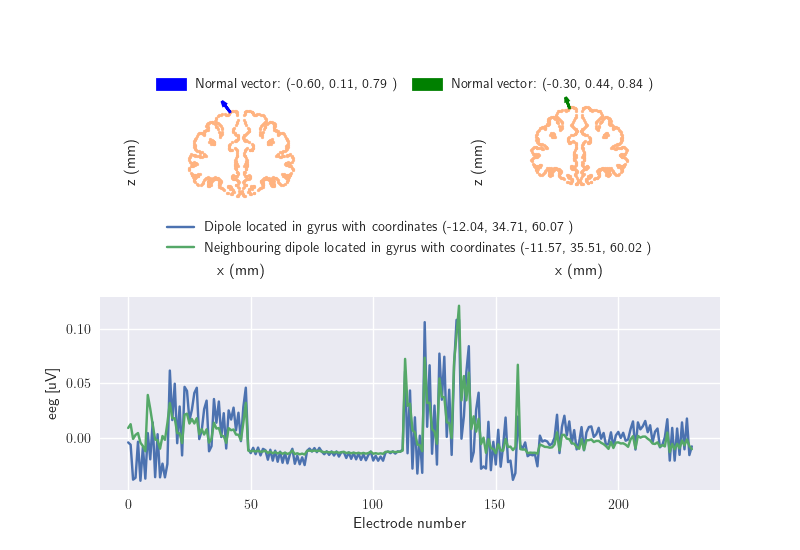
\includegraphics[width=\linewidth]{figures/neighbour_dipoles.png}
    \caption{EEG signal for neighbouring dipoles.}
    \label{fig:neighbour_dipoles}
\end{figure}

However, in order to decribe the effect of the \emph{orientation} of the dipoles relative to the EEG electrodes, we have in Figure \ref{fig:gyrus_and_sulcus_EEG} provided the EEG signals from two manually chosen dipole locations in the New York head model. The two dipoles illusrated are located in a gyrus and in a sulcus, both providing a different EEG outcome. In general, the EEG signal contribution from a single current dipole is maximized if the dipole is located in a gyrus, perpendicular oriented. Such a case is depiced in Figure \ref{fig:gyrus_and_sulcus_EEG}B. However, if we place a dipole in a sulcus, again with perpendicular orientation, we can observe a substantial EEG contribution, but in contrast to the dipole in the gyrus we notice a more dipolar pattern \ref{fig:gyrus_and_sulcus_EEG}C.

\begin{figure}[!htb]
    \centering
    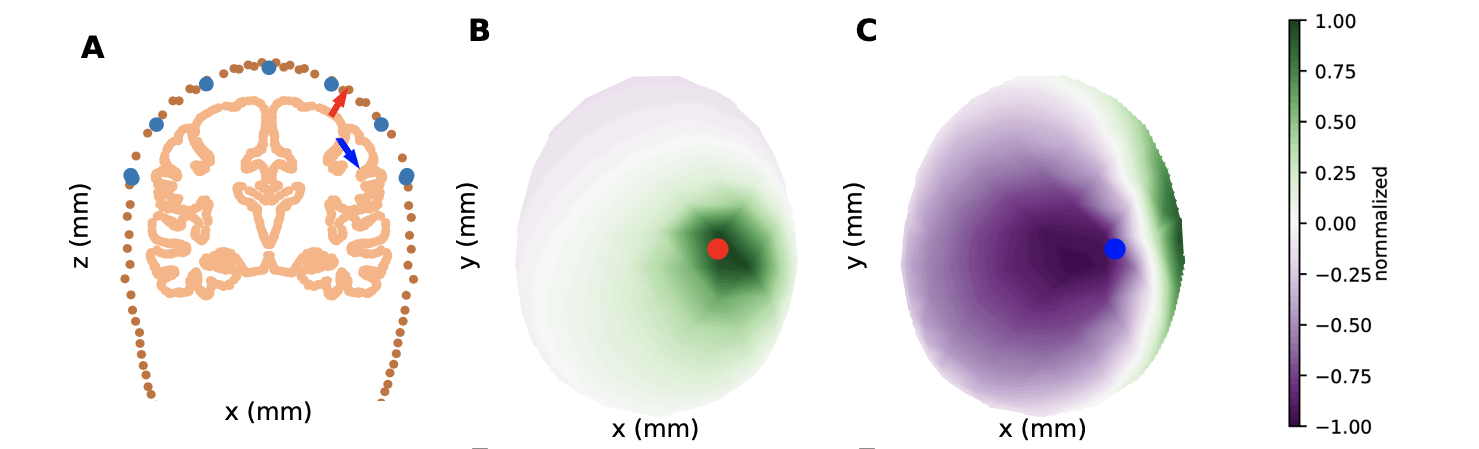
\includegraphics[width=\linewidth]{figures/gyrus_and_sulcus_EEG.png}
    \caption{A: Two manually chosen dipole locations in the New York head model, located in a gyrus (red) and a sulcus (blue). The head model is seen from the side (x, z-plane). EEG electrode locations close to the chosen cross section plane are marked in light blue. The available dipole locations close to the cortical cross section effectively draw an outline of the cortical sheet, and are marked in pink. The current dipole moment was in all cases $10^7$ nA$\mu$m. B: Interpolated color plot of EEG signal from the dipole in gyrus, seen from the top (x, y-plane). The plotted EEG signal is normalized but the maximal value was 1.1 $\mu$V. C: Interpolated color plot of EEG signal from the dipole in sulcus. The plotted EEG signal is normalized but the maximal value was 0.7 $\mu$V. (source: BookTVN)}
    \label{fig:gyrus_and_sulcus_EEG}
\end{figure}
\\
\\


\subsection{Noise}
As for all experimental data, real EEG recordings contain noise. Artifacts are signals recorded by EEG but with a origin different from those generated by human brain activity. As some artifact may mimic true epileptiform abnormalities or seizures, awereness of artifacts and methods for distinguishing such signals from brain waves is highly important (\url{https://link.springer.com/chapter/10.1007/978-3-030-03511-2_8}).

There are two different dypes of artifacts, classified according to their origin. Physiological artifacts originate from the patient itself, where the most usual ones are ocular activity, muscle activity, cardiac activity, perspiration and respiration. Technical artifacts, on the other hand, is generated from the environment of the patient, such as cable and body movements or electromagnetic interferences. (\url{https://www.bitbrain.com/blog/eeg-artifacts}).

Filtering techniques are usually utilized in order to remove artifact from EEG before analyzation of the recordings. But, when it comes to the simulated EEG data of ours, we are in no need to remove such noise, as there simply is none. The simulated EEG data can be understood as already filtered data that has undergone preprocessing steps, to ensure a high signal-to-noise ratio (\url{https://en.wikipedia.org/wiki/Signal-to-noise-ratio}). Moreover we understand the simulated data as an averaged measure of the typical EEG time series. However, in order to avoid overfiting and for other tecnical detailes, we do need to ass noise to tha data before feeding it to the neural network. Therefore, to the final dataset of ours we add normally distributed noise of 10 $\%$, with mean .... and standard deviation ... .


\section{Localizing Single Dipole Sources}

\subsection{The dataset}
The data set used to train a simple feed forward neural network consists of 10 000 rows, where each row corresponds to one sample, or let us say - one patient. Within the data set we have 231 columns, also referred to as features, representing the EEG measure at every recording electrode. Thus, we are left with a design matrix of size 10 000 x 231.

An example of how the input EEG data may look like for one sample (before adding noise) is provided in figure \ref{fig:eeg_field_1_dipole_example}. The figure illustrates the EEG result from a sample containing a single current dipole source at a random position within the celebral cortex. As also can be seen from the characteristic dipolar pattern, the dipole is located in a sulcus. The EEG measure is seen from both sides (x-, z-plane and y-, z-plane) and above (the x-, y-plane). EEG electrode locations are presented as filled circels, where the color of the fill represents the amplitude of the measured signal for the given electrode. The position of the current dipole moment is marked with a yellow star. As can be read off from the figure, the EEG signals, for this given sample, range from between -1 to 1 $\mu V$.

% How it looks when we add noise.
% Maybe add arrow and dipole direction??
\begin{figure}[!htb]
    \centering
    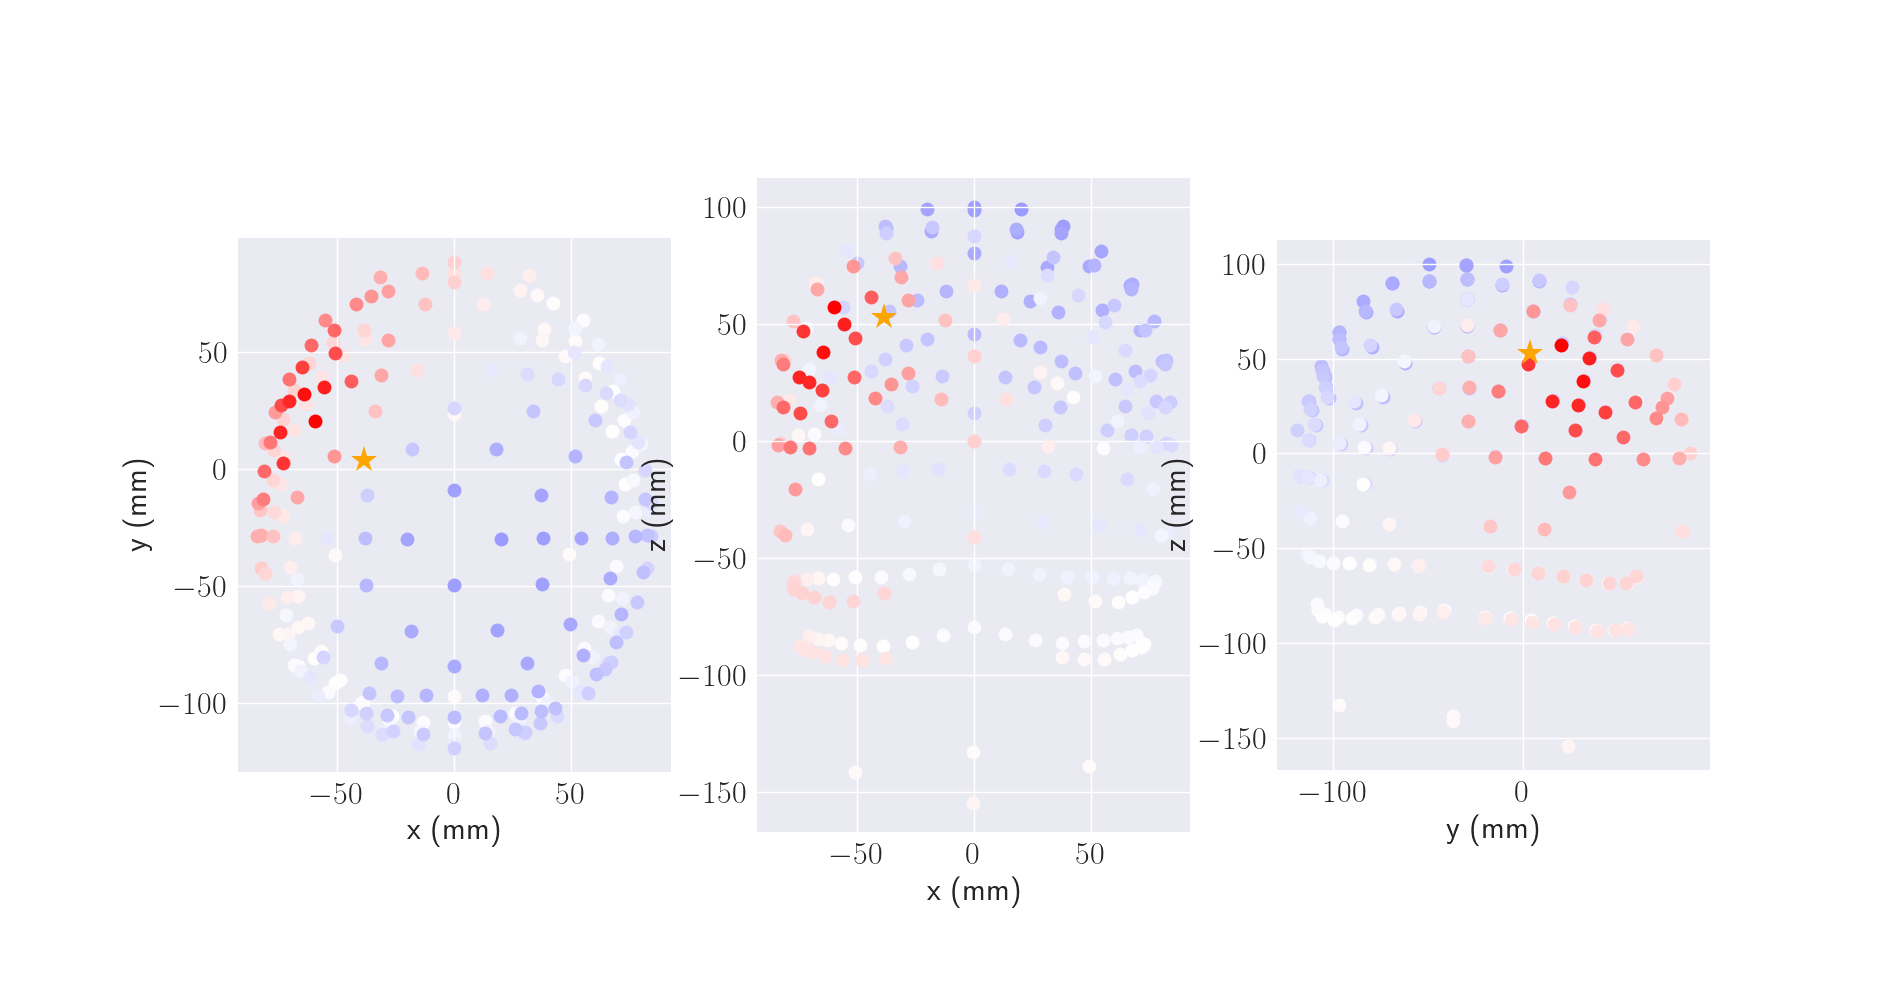
\includegraphics[width=\linewidth]{../Code/plots/finals/eeg_field_1_1.png}
    \caption{EEG for a sample containing one single current dipole source at a random position within the celebral cortex. The EEG measure is seen from both sides (x-, z-plane and y-, z-plane) and above (the x-, y-plane). EEG electrode locations are presented as filled circels, where the color of the fill represents the amplitude of the measured signal for the given electrode. The position of the current dipole moment is marked with a yellow star.}
    \label{fig:eeg_field_1_dipole_example}
\end{figure}

\subsection{Validation accuracy}
In Figure \ref{fig:single_dipole_accuracy} we have provided the validation accuray, using mean squared error (MSE) and the coefficient of determination (R2-score).

The expression for MSE when predicting the x-, y- and z-coordinate, goes as follows:

\begin{equation}
MSE(\hat{y},\hat{\tilde{y}}) &= \frac{1}{n}
\sum_{i=1}^{n}(y_i-\tilde{y}_i)^2 \\
&= \frac{1}{3}\sum_{i=1}^{3}((x-\tilde{x})^2 + (y-\tilde{y})^2 + (z-\tilde{z})^2 )
\label{eq:MSE}
\end{equation}

The coefficient of determination is given as follows:
\begin{equation}
R^2(\hat{y}, \tilde{\hat{y}}) = 1 - \frac{\sum_{i=0}^{n - 1} (y_i - \tilde{y}_i)^2}{\sum_{i=0}^{n - 1} (y_i - \bar{y})^2},
\label{eq:R2}
\end{equation}

Where the mean value of $y_i$ is defined by $\bar{y}$:

\begin{equation*}
\bar{y} =  \frac{1}{n} \sum_{i=0}^{n - 1} y_i.
\label{eq:ybar}
\end{equation*}


\begin{figure}[!htb]
    \centering
    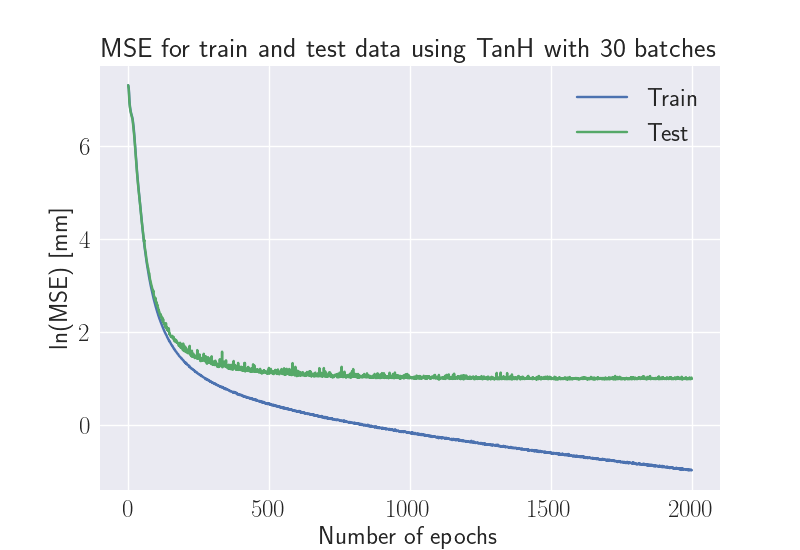
\includegraphics[width=\linewidth]{../Code/plots/finals/MSE_NN_1_10000_TanH_30_2000.png}
    \caption{The validation accuracy for the simple Feed Forward Neural Network with 10 000 samples with tanh activation function. }
    \label{fig:single_dipole_accuracy}
\end{figure}

\begin{figure}[!htb]
    \centering
    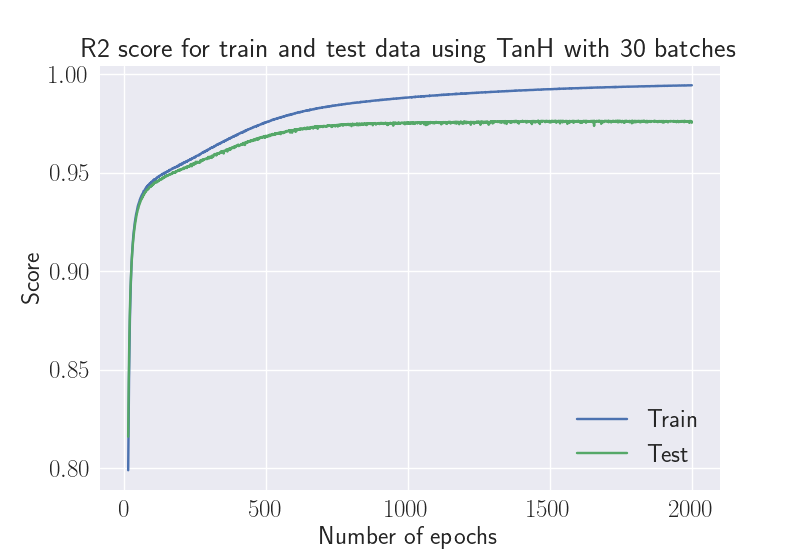
\includegraphics[width=\linewidth]{../Code/plots/finals/R2_NN_1_10000_l1_TanH_30_2000.png}
    \caption{The R2 score for the simple Feed Forward Neural Network with 10 000 samples with tanh activation function. }
    \label{fig:single_dipole_R2}
\end{figure}

\begin{figure}[!htb]
    \centering
    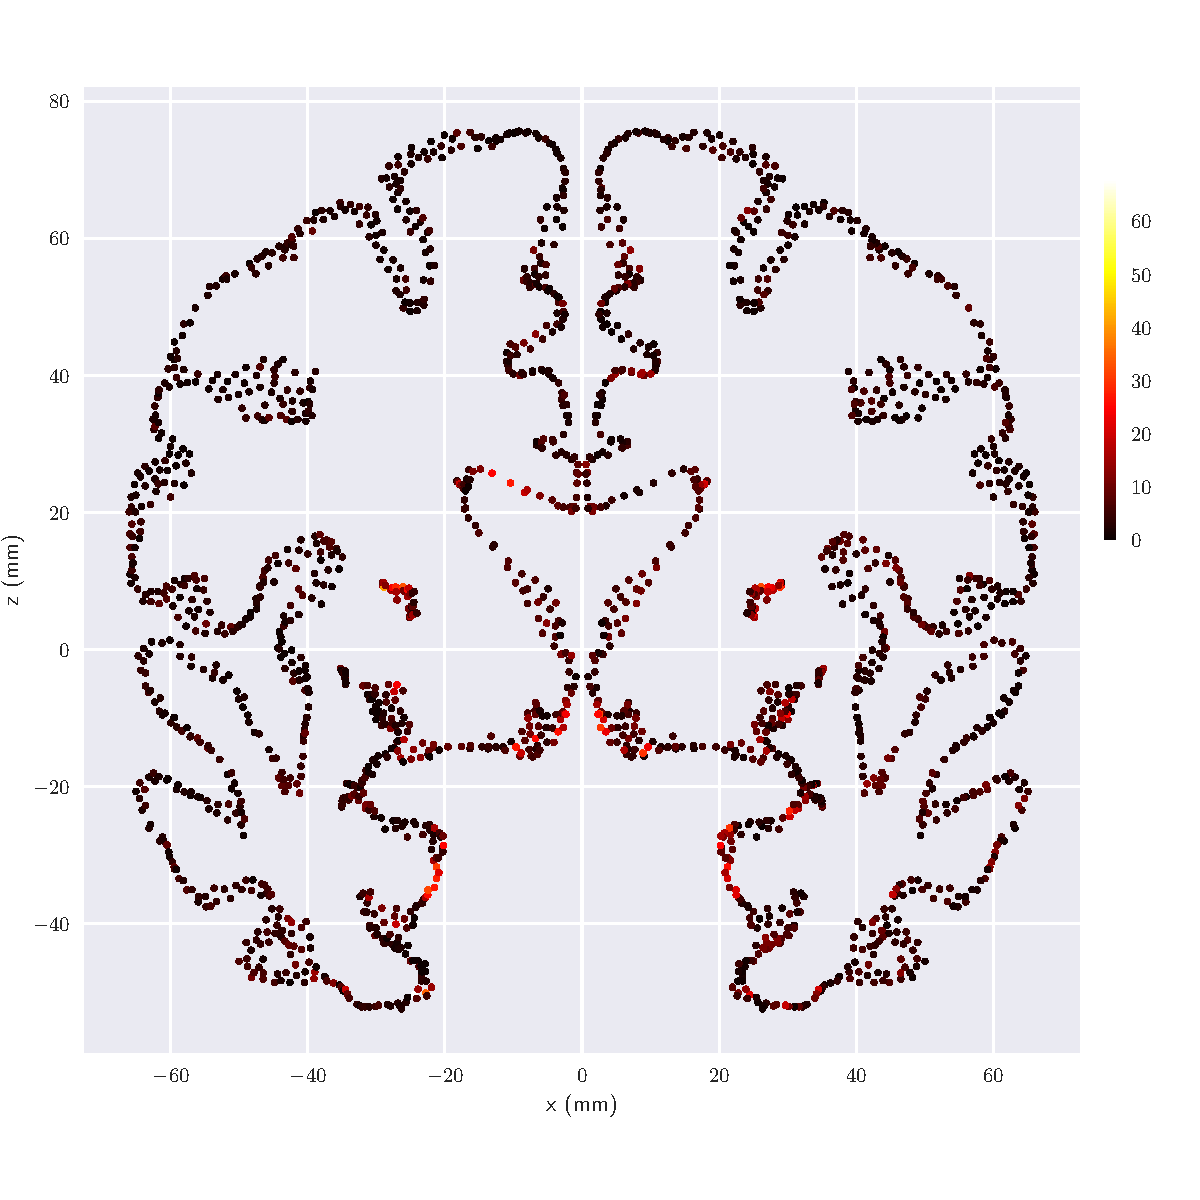
\includegraphics[width=\linewidth]{../Code/plots/finals/mse_y_plane.pdf}
    \caption{The mean squared error of the location accuracy (NN) at different dipole locations
    in the y cross section, for the simple Feed Forward Neural Network.}
    \label{fig:single_dipole_accuracy_plane}
\end{figure}



% \begin{figure}[!htb]
%     \centering
%     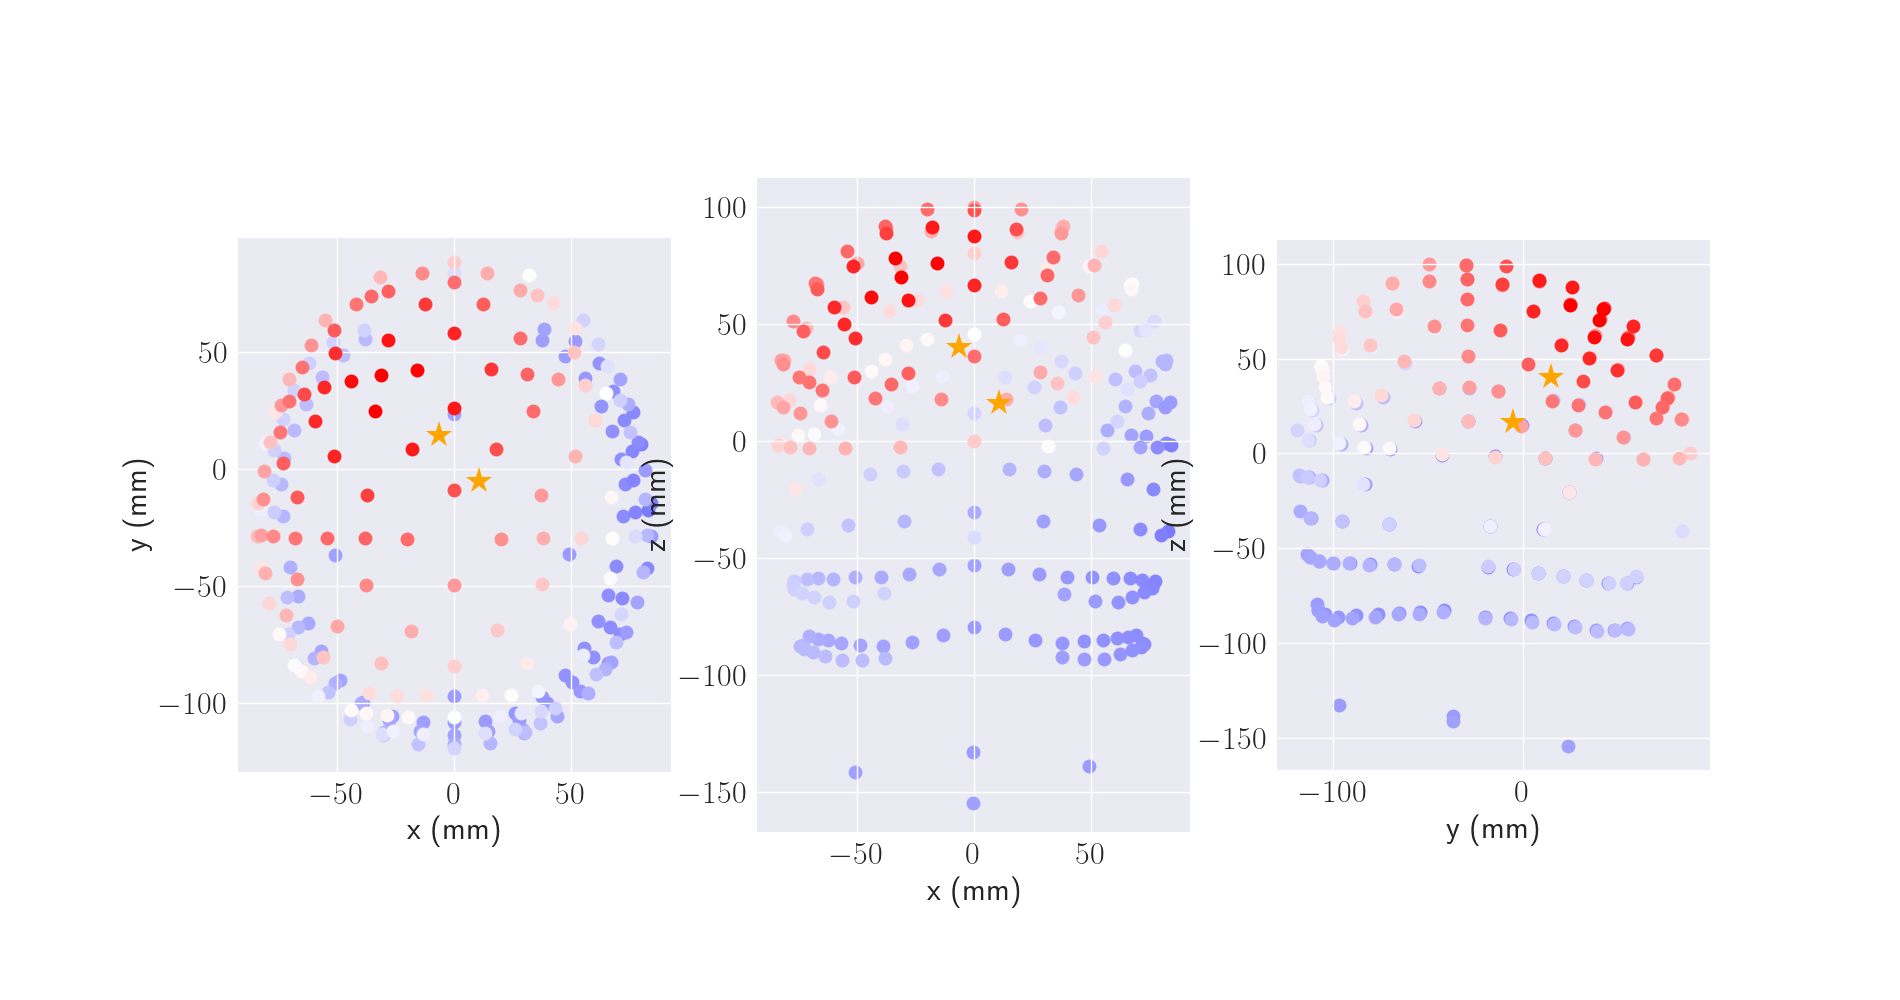
\includegraphics[width=\linewidth]{../Code/plots/finals/eeg_field_2_2.png}
%     \caption{Example 2 dipoles. }
%     \label{fig:eeg_field_2_dipole_example}
% \end{figure}



% \begin{figure}[!htb]
%     \centering
%     \includegraphics[width=\linewidth]{../Code/plots/NN/MSE_NN_noise_TanH_100_3000.png}
%     \caption{The validation accuracy for simple Feed Forward Neural Network with 10 000 samples with tanh activation function and 10$\%$ noise added to the data. }
%     \label{fig:single_dipole_accuracy}
% \end{figure}




\section{Convolution Neural Network Approach for localizing single dipole sources}

Some results for the prediction of location for single current dipoles.


\begin{figure}[!htb]
\centering
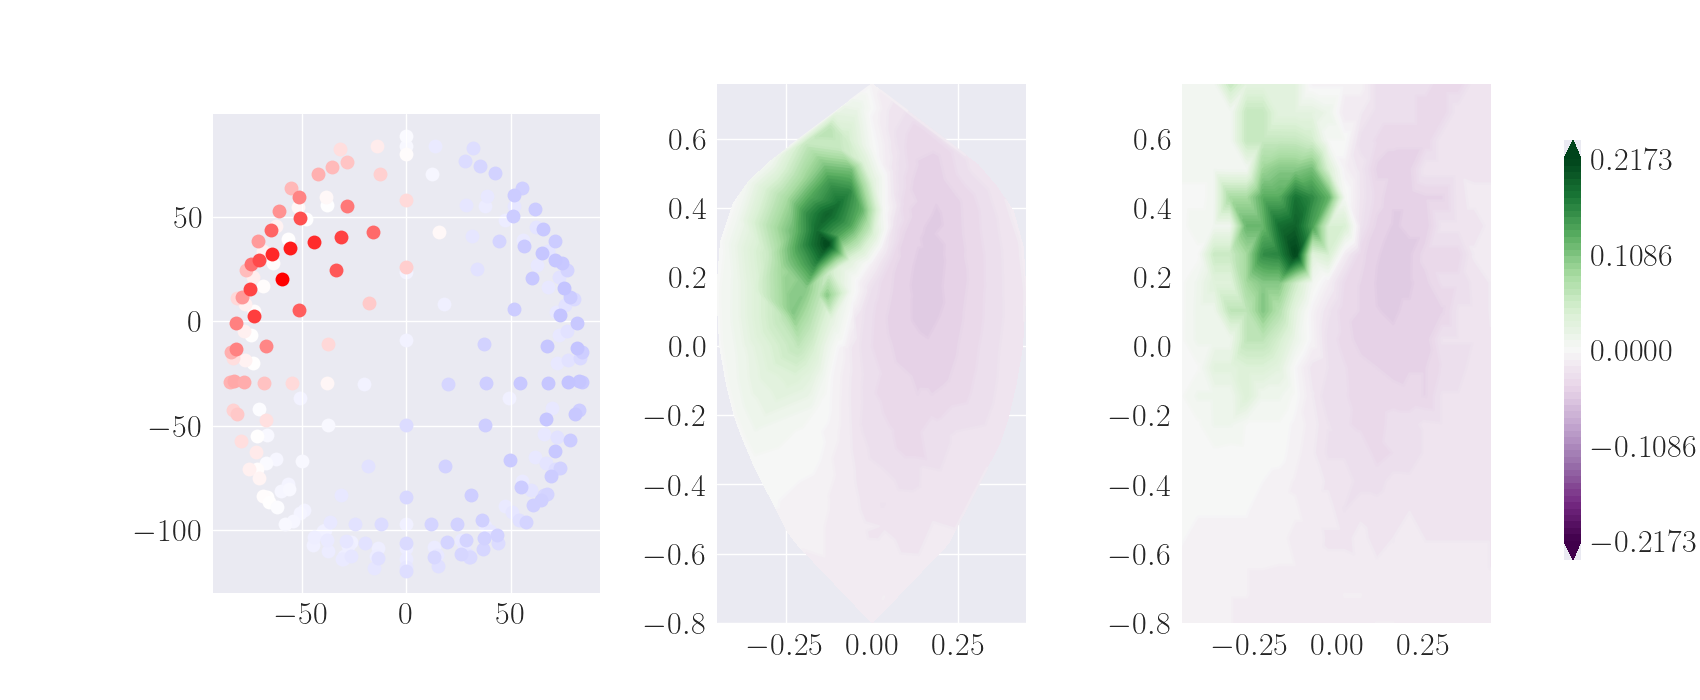
\includegraphics[width=\linewidth]{../Code/plots/finals/new_eeg_dipole_pos_0.png}
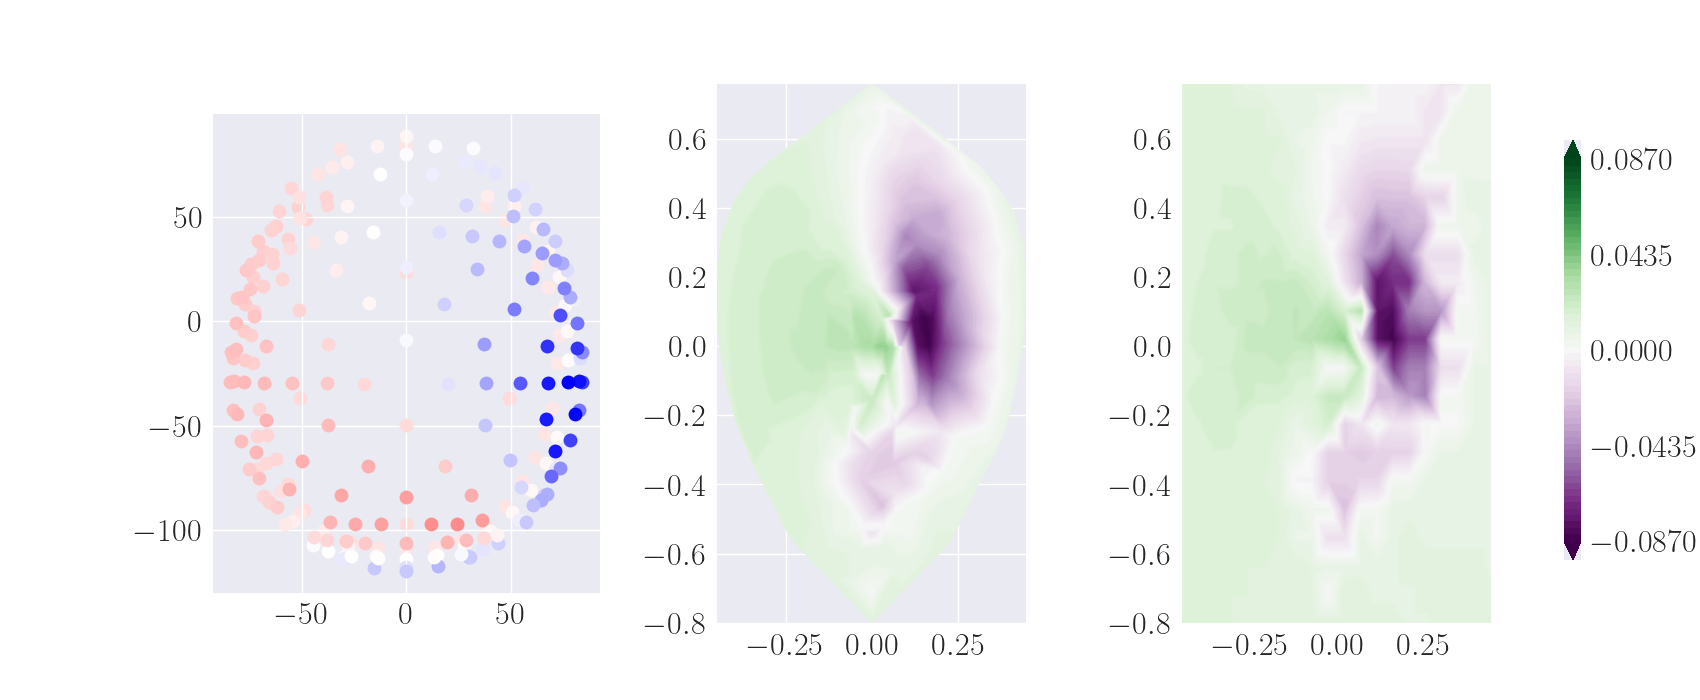
\includegraphics[width=\linewidth]{../Code/plots/finals/new_eeg_dipole_pos_4.png}
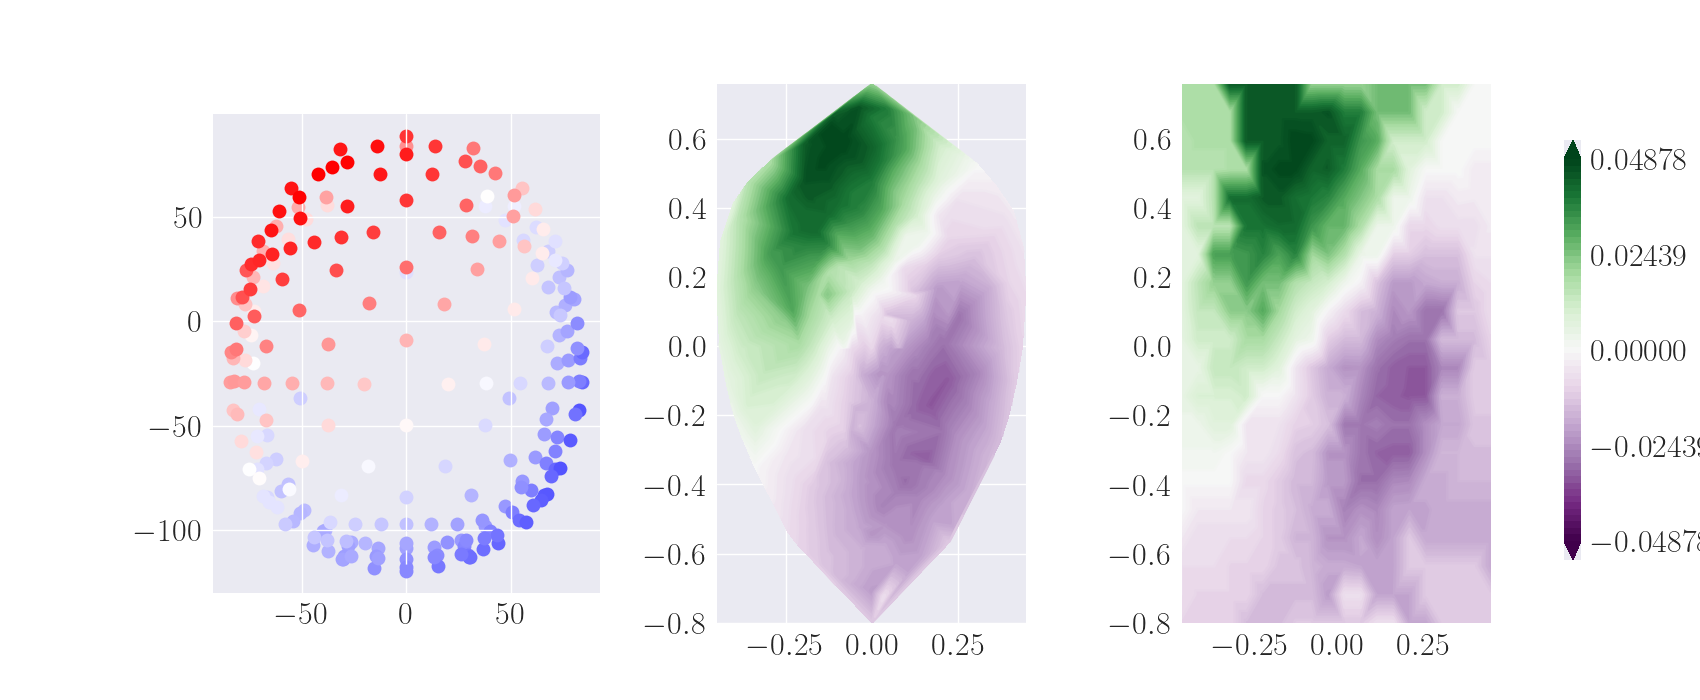
\includegraphics[width=\linewidth]{../Code/plots/finals/new_eeg_dipole_pos_6.png}

\caption{\newline
\textbf{Right}: EEG measure for 3 different samples measured in $\mu V$. \newline
\textbf{Middle and Left}: Illustration of the interpolation of the EEG data into two-dimensional matrix.}
\label{fig:eeg_dipole_pos_0}

\end{figure}

\begin{figure}[!htb]
    \centering
    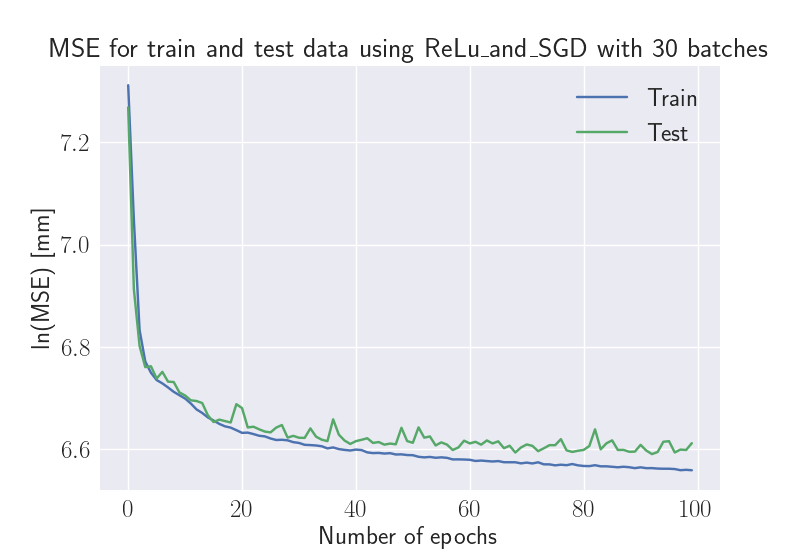
\includegraphics[width=\linewidth]{../Code/plots/finals/MSE_CNN_dipoles_2_interpolated_CNN_20x20_10000_ReLu_and_SGD_30_100.png}
    \caption{The validation accuracy for Convolutional Neural Network with 10 000 samples (20x20 matrix) with ReLU activation function. }
    \label{fig:single_dipole_accuracy_CNN_2d}
\end{figure}

% \begin{figure}[!htb]
%     \centering
%     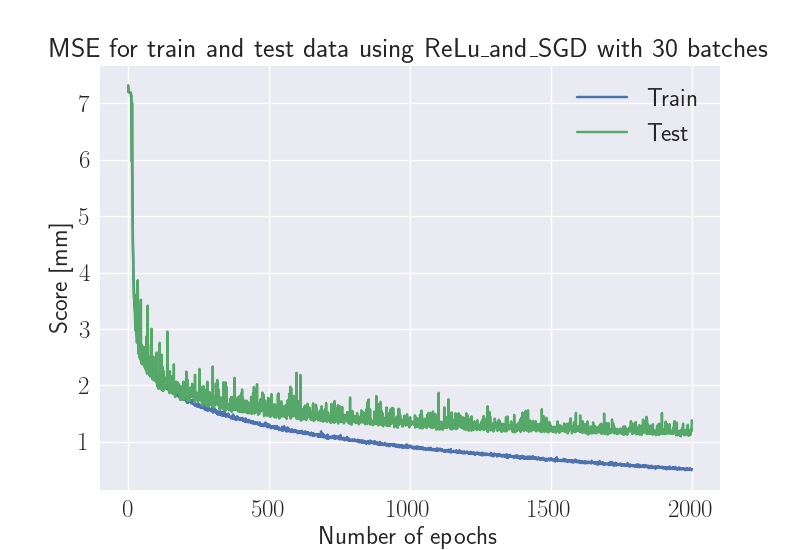
\includegraphics[width=\linewidth]{../Code/plots/CNN/MSE_interpolated_CNN_20x20_10000_ReLu_and_SGD_30_2000.png}
%     \caption{The validation accuracy for Convolutional Neural Network with 10 000 samples (20x20 interpolated matrix) with ReLU activation function. }
%     \label{fig:single_dipole_accuracy_CNN}
% \end{figure}


\section{Region of Active Correlated Current Dipoles}

Some results for the prediction of the size and location of current dipole populations.

\begin{figure}[!htb]
    \centering
    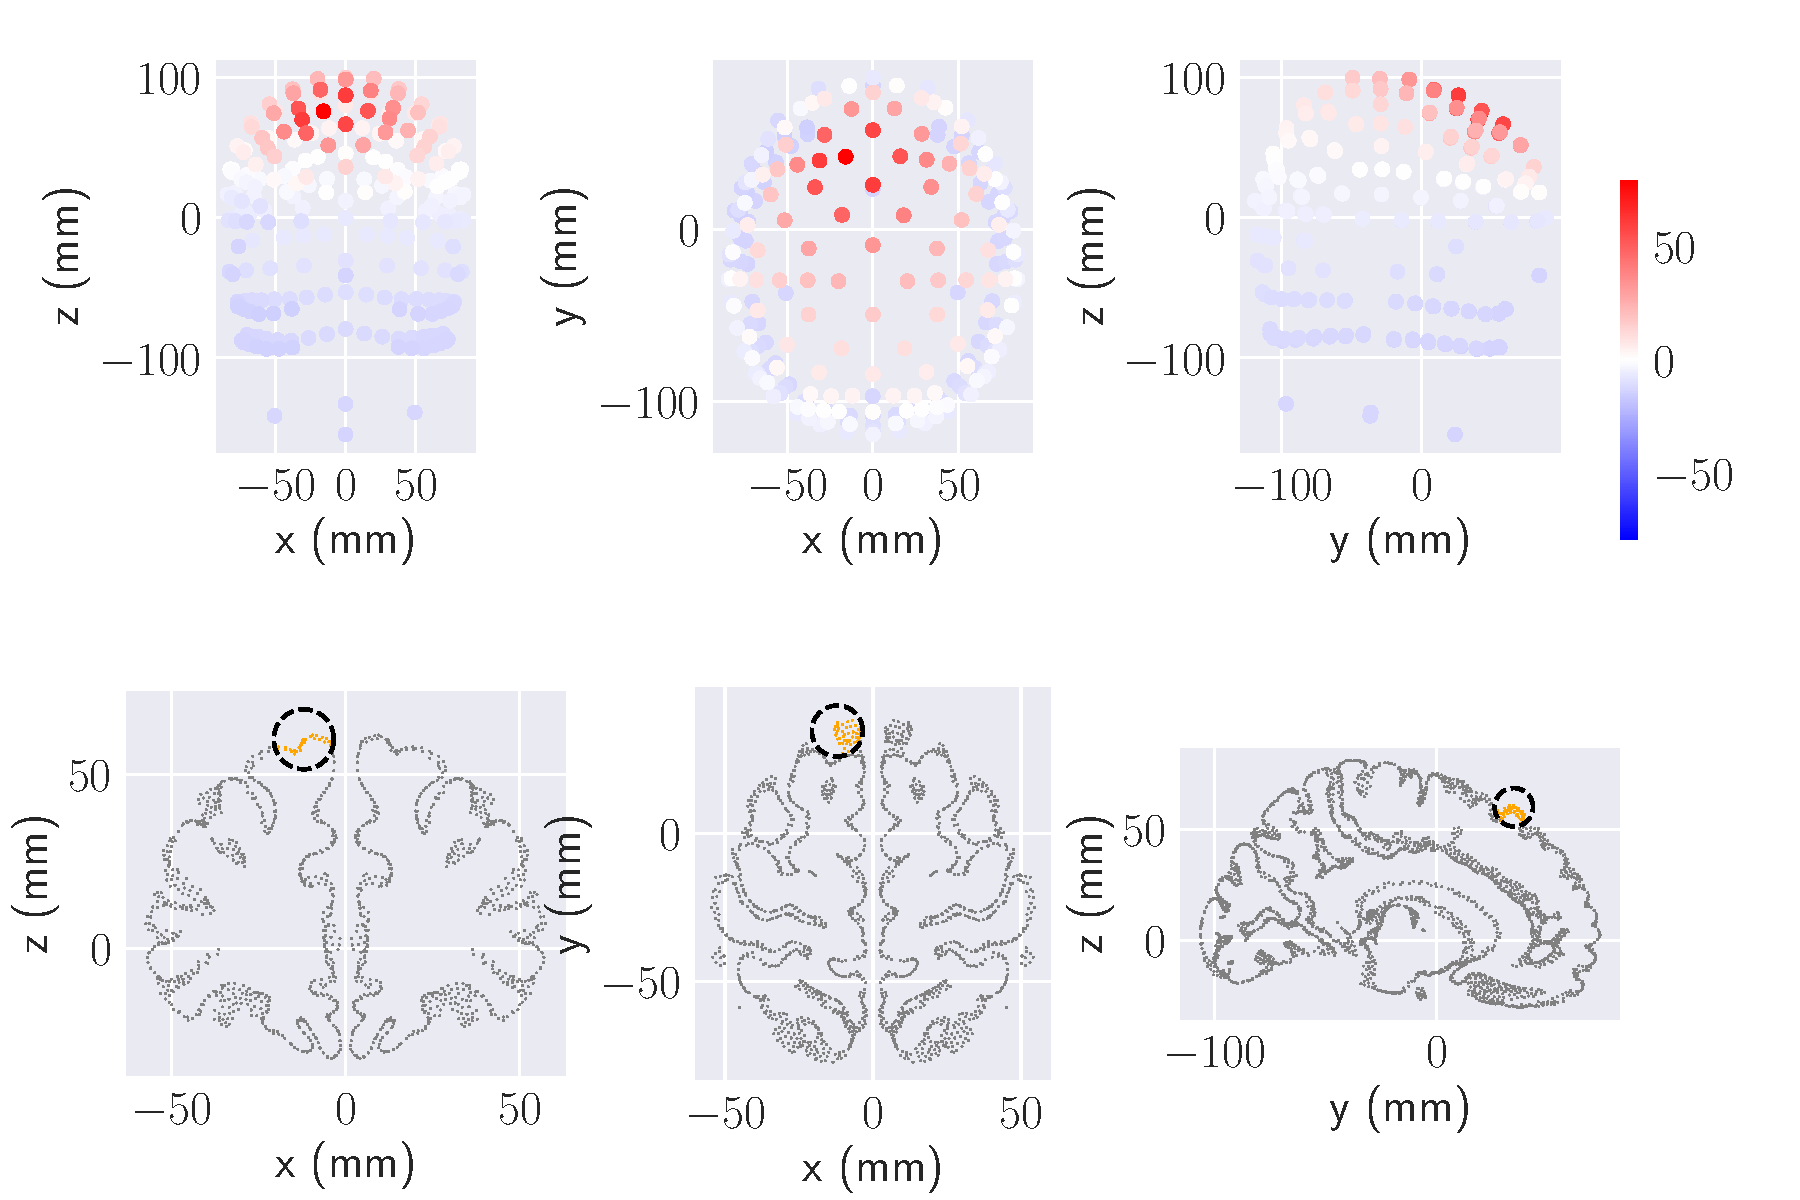
\includegraphics[width=\linewidth]{../Code/plots/finals/new_dipole_area_reduced_0.pdf}
    \caption{EEG for a sample containing a spherical population of current dipole sources with a random center within the celebral cortex. The EEG measure is seen from both sides (x-, z-plane and y-, z-plane) and above (the x-, y-plane). EEG electrode locations are presented as filled circels, where the color of the fill represents the amplitude of the measured signal for the given electrode.}
    \label{fig:dipole_area}
\end{figure}

\begin{figure}[!htb]
    \centering
    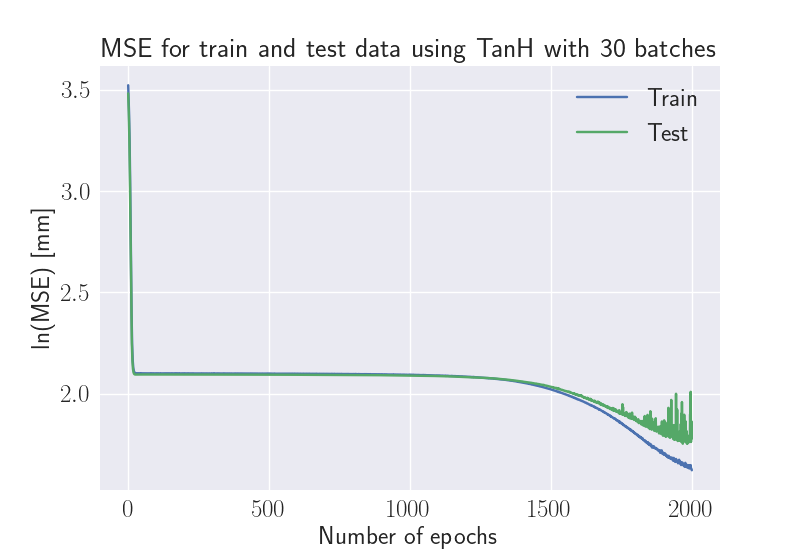
\includegraphics[width=\linewidth]{../Code/plots/finals/normalized_dipole_area.png}
    \caption{The validation accuracy for the simple Feed Forward Neural Network, predicting both center and radius for 10 000 samples, for 2000 epochs, with a learning rate equal to 0.0001.}
    \label{fig:dipole_area_result}
\end{figure}

\begin{figure}[!htb]
    \centering
    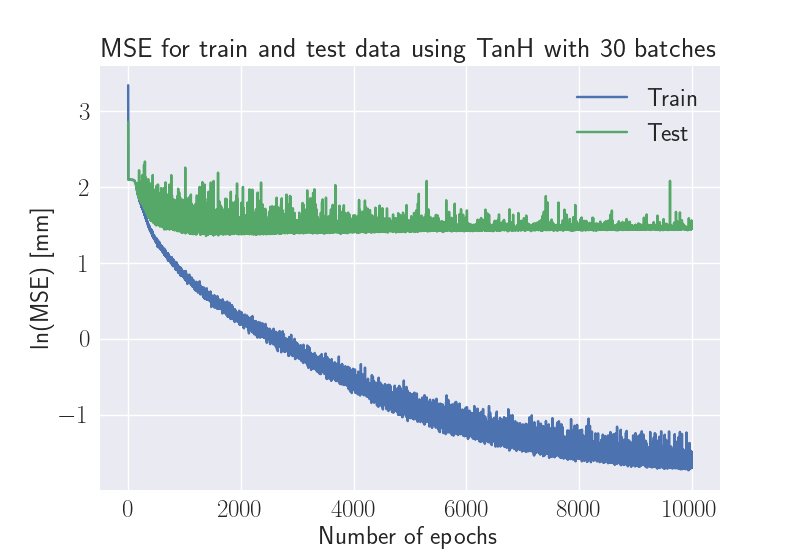
\includegraphics[width=\linewidth]{../Code/plots/finals/MSE_dipole_area_lr0.001_l1_20mm_TanH_30_10000.png}
    \caption{The validation accuracy for the simple Feed Forward Neural Network, predicting both center and radius for 10 000 samples, for 10000 epochs, with a learning rate equal to 0.001.}
    \label{fig:dipole_area_result}
\end{figure}


Printed in terminal:

Epoch 9898/9999 | Train:  0.187 | Test:  4.275

Epoch 9899/9999 | Train:  0.184 | Test:  4.288

Epoch 9900/9999 | Train:  0.201 | Test:  4.279


Target: tensor([-1.0800, -1.9594,  0.4290, 11.0140])

Predicted: tensor([-1.1171, -1.9642,  0.4575, 16.5920])


Target: tensor([-6.7642e-02,  1.5426e+00, -1.0356e-02,  1.5576e+01])

Predicted: tensor([-0.3908,  1.4285, -0.1167, 15.9222])


Target: tensor([-0.6671, -1.0569,  1.8694,  7.1385])

Predicted: tensor([-0.7248, -1.0950,  1.9903,  6.2405])



\section{Localizing Multiple Dipole Sources}
\begin{figure}[!htb]
    \centering
    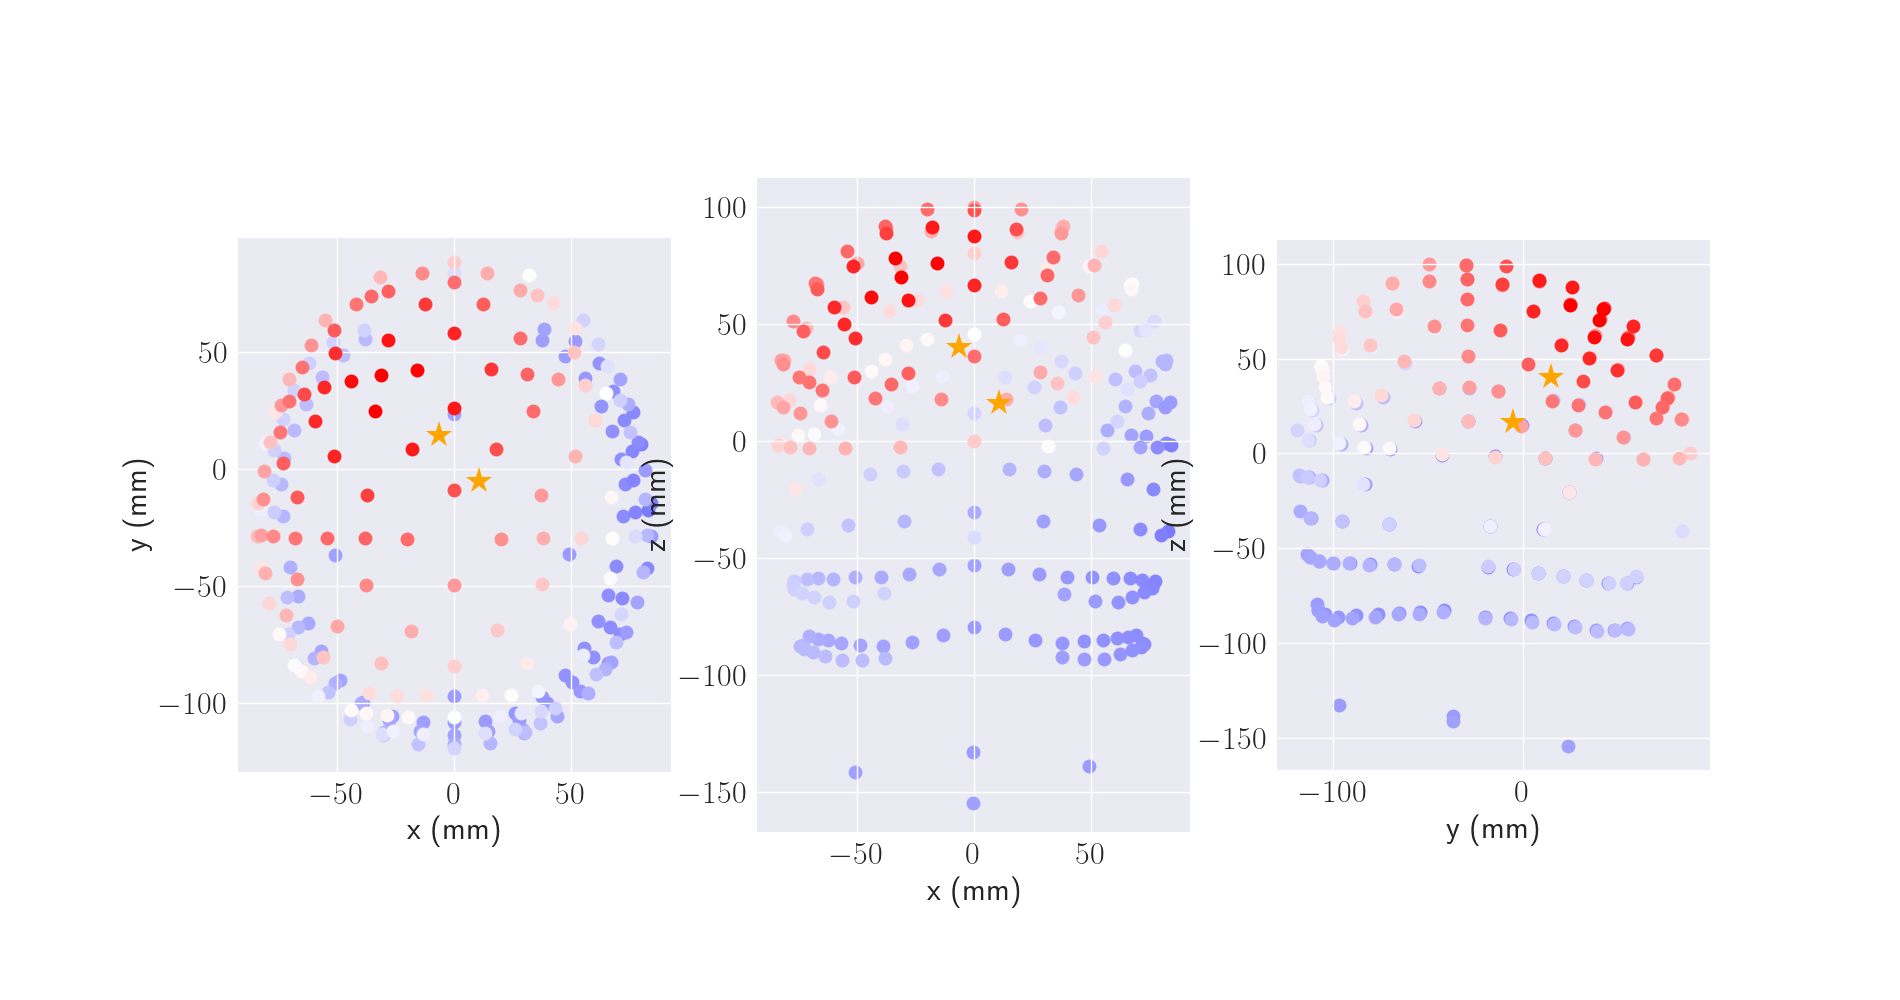
\includegraphics[width=\linewidth]{../Code/plots/finals/eeg_field_2_2.png}
    \caption{EEG for a sample containing two current dipole sources at random positions within the celebral cortex. The EEG measure is seen from both sides (x-, z-plane and y-, z-plane) and above (the x-, y-plane). EEG electrode locations are presented as filled circels, where the color of the fill represents the amplitude of the measured signal for the given electrode. The positions of the current dipole moments are marked with yellow stars.}
    \label{fig:dipole_area_result}
\end{figure}

\begin{figure}[!htb]
    \centering
    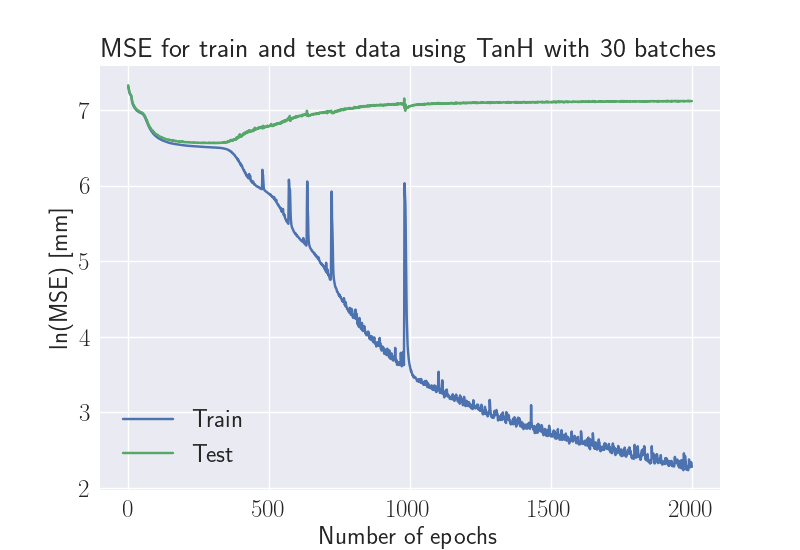
\includegraphics[width=\linewidth]{../Code/plots/finals/MSE_NN_2_10000_l1_TanH_30_2000.png}
    \caption{The validation accuracy for the simple Feed Forward Neural Network, predicting two current dipole sources.}
    \label{fig:dipole_area_result}
\end{figure}

\end{document}

% results, simple dipole, convolutional 
% !TEX root = main.tex
\documentclass[a4paper, UKenglish, 11pt]{uiomaster}
\usepackage{lipsum}
\usepackage[subpreambles=true]{standalone}
\usepackage[table,xcdraw]{xcolor}

\begin{document}

\chapter{Localizing Single Current Dipole Sources} \label{chap:simple_dipole_FFNN}
\rednote{Figure texts not fixed jet}
In this chapter, we will delve into the performance of the fully connected feed-forward neural network (FCNN) in solving the inverse problem. Our primary focus centers on investigating whether the accuracy of the neural network can be linked to the precise positioning and orientation of the current dipoles it is tasked with identifying or if the performance remains consistent across all brain regions and structures. Moreover, we shall employ a range of diverse error metrics to rigorously evaluate the performance of the network in this task.


\section{EEG Sensitivity of Dipole Location and Orientation}
According to Ness et al. (2021) \cite{naess2021biophysically}, EEG signals demonstrate limited sensitivity to minor shifts in the precise location of neural current dipoles. This insensitivity can be attributed to the considerable separation between EEG electrodes and cortical neural sources compared to the dimensions of individual neurons and the thickness of the human cortex. Before evaluating the overall performance of our network, our investigation seeks to ascertain whether neighboring neural dipoles yield nearly indistinguishable EEG signals or exhibit noticeable distinctions. This exploration provides valuable insights into the network's ability to handle the complexity of the problem. If two dipoles located only 1 mm apart yield nearly identical results, it signifies a commendable performance by the network if it ables to distinguish at this scale. We emphasize that  in this context, ''neighboring'' is defined based on the resolution of the NYHM. To assess the similarity in EEG signals between nearby dipoles, we employ the Pearson correlation coefficient.

The Pearson correlation coefficient is a statistical measure that quantifies the relationship between two variables. It is defined as the ratio of the covariance of the two variables to the product of their standard deviations. The coefficient ranges from -1 to 1, with -1 denoting a perfect negative correlation and 1 indicating a perfect positive correlation. A coefficient of 0 signifies the absence of a linear relationship between the variables \cite{numpy-docs}.

In Figure \ref{fig:neighbour_dipoles}, we present EEG signals corresponding to dipoles located in close proximity within the New York Head Model's cortical matrix. The upper panel illustrates the two distinct EEG signals originating from the blue and green dipoles, while the lower panel shows the EEG signal corresponding to the blue and red dipoles. The blue central dipole is positioned between the green and red dipoles, located at the leftmost and rightmost positions in the NYHM cortical matrix, respectively. The Euclidean distance between the blue and green dipoles is 0.914 mm, while the blue and red dipoles are separated by 1.926 mm.

In Figure \ref{fig:neighbour_dipoles}, the EEG signals of the blue and green dipoles exhibit significant overlap, with a high correlation coefficient of 0.966, indicating a strong positive relationship. In contrast, the EEG signals of the blue and red dipoles show less resemblance, with a correlation coefficient of 0.695, indicating a weaker linear relationship.

The observed variability in the correlation between the EEG signals of neighboring dipoles can be attributed to differences in the orientation of their respective dipole's normal vectors. The observed smaller value in the correlation matrix between the red and blue dipole, in contrast to the higher correlation between the blue and green dipole, is related to the more pronounced angular disparity in the normal vector alignment between the red dipole and the blue dipole. In contrast, there is a relatively smaller angular difference observed between the green dipole's normal vector and that of the blue dipole.

The distinct differences in the orientation of normal vectors arise from constraints imposed during data generation, which are designed to ensure that dipole orientations remain perpendicular to the complex folding of the cerebral cortex. As a result, neighboring dipoles within the NYHM possess distinct normal vectors, potentially leading to significantly different simulated EEG signals.

Furthermore, it is important to note that the separation between the red dipole and the blue dipole is somewhat greater than the distance between the blue and green dipoles. This variation in separation can be attributed to the specific construction of the NYHM cortex, as established by its developers.

In conclusion, these findings underscore the intricate nature of EEG signals, where the correlation analysis reveals varying degrees of similarity for neighboring dipoles. In some scenarios, it becomes evident that the linear relationship between EEG signals originating from distinct dipoles is relatively small, suggesting the network's capability to separate the EEG signals. In other instances, the EEG signals exhibit significant similarity, which may pose a challenge for the network in distinguishing them.


%Despite the common belief that neurons in the upper cortical layers would dominate the EEG due to their proximity to the electrode compared to neurons in deeper layers, such location differences do not significantly affect the EEG signals. This phenomenon can be explained by the fact that the low conductivity of the skull introduces a spatial low-pass filtering effect, which mitigates the impact of location discrepancies.
% Maybe what is meant here is that we therefore only consider the outer corical surface

\begin{figure}[!htb]
    \centering
    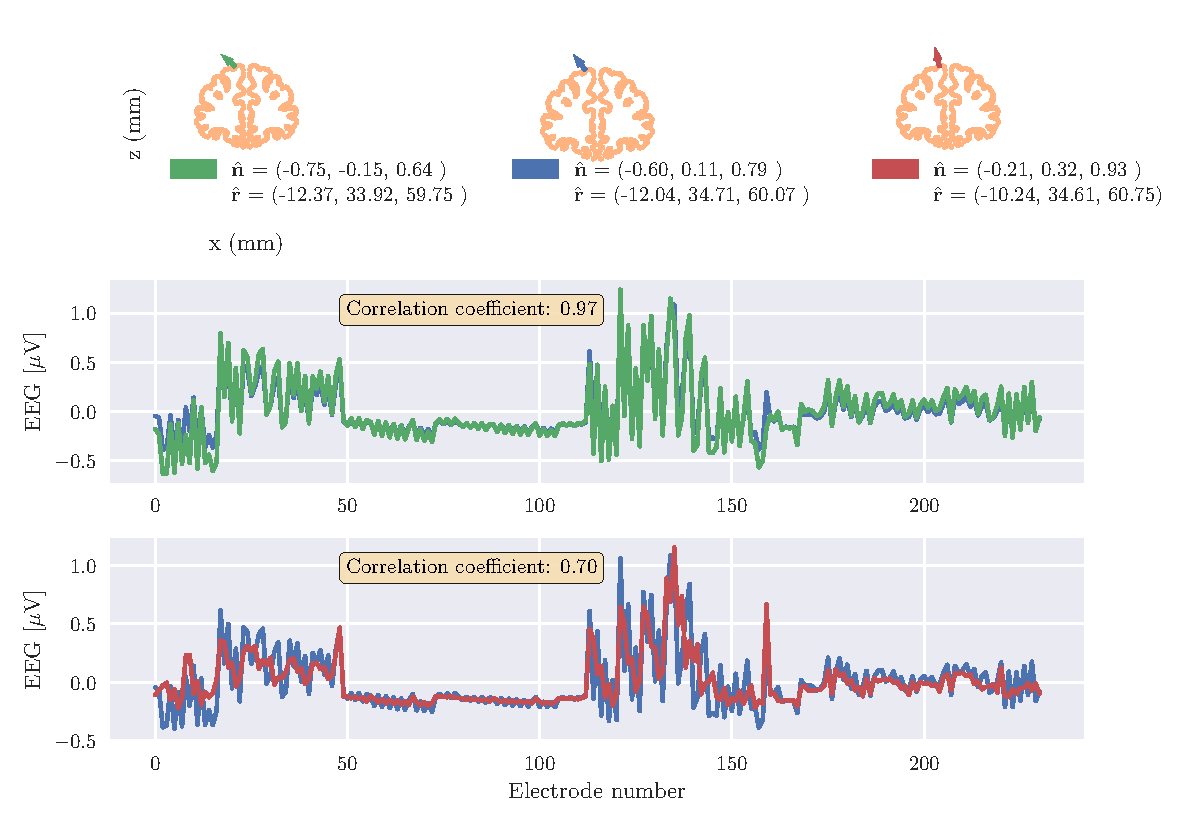
\includegraphics[width=\linewidth]{figures/compare_dipoles.pdf}
    \caption{EEG signals plotted against electrode number for three neighbouring dipoles with normal vectors (-0.60, 0.11, 0.79), (-0.75, -0.15, 0.64), (-0.21, 0.32, 0.93) and positions (-12.04, 34.71, 60.07), (-12.37, 33.92, 59.75), (-10.24, 34.61, 60.75). The correlation coefficient between the blue and green dipole is 0.97, while it is 0.70 for the blue and red dipole. \rednote{Which coordinate system? Where is (0,0,0) located?}}
    \label{fig:neighbour_dipoles}
\end{figure}

\FloatBarrier

\section{Performance Evaluation} \label{sec:performace_evaluatoin}
\rednote{Move to training chapter?}
Based on the findings of Akalin Acar and Makeig 2013 \cite{akalin2013effects} and Biasiucci et al. 2019 \cite{biasiucci2019electroencephalography}, source localization using spherical head models typically yields localization errors in the range of 10-30 mm. On the other hand, the utilization of modern subject-specific head models is expected to result in errors of less than 10 mm. The New York Head Model falls within the second category, and we will, therefore, let 10 mm serve as our guideline when evaluating the network's predictions.

Nevertheless, we emphasize that our primary objective is not necessarily the development of a flawless neural network for immediate clinical applications. Our aim is to ascertain whether a simple fully connected feed-forward neural network can effectively discern patterns and approximate dipole positions based on the simulated EEG data, collected using LFPy and the integrated Head Model, as outlined in Chapter 3.

Within this section, we will employ various techniques to assess the network's performance. This evaluation will include tracking the loss during training, utilizing different sets of error metrics to calculate the average prediction error, and determining the distribution of test samples falling within predefined threshold values.

\subsection{Results from Training and Validation Process}
The FCNN underwent 500 epochs of training, and the convergence of the mean Euclidean distance (MED) is illustrated in Figure \ref{fig:single_dipole_accuracy}. The entire training process, encompassing data loading and preprocessing, took approximately 1.5 hours, with each epoch having an average training duration of about 11.00 seconds.

The validation loss exhibited a noticeable stabilization trend after approximately 350 epochs. At this point, the training could have been terminated. However, we chose to continue training for the full 500 epochs to confirm that no further improvements in validation data performance were attainable and to emphasize the network's full convergence.

Figure \ref{fig:single_dipole_accuracy} visually demonstrates a clear reduction in loss, indicating the network's effective learning of patterns in the data. Validation loss stabilization becomes evident around the 350-epoch mark, while the training loss continues to decrease until it stabilizes between 400 and 500 epochs. This observation suggests that the model did not demonstrate signs of overfitting, as the validation loss remained constant, and the training loss ultimately stabilized. At epoch 500, the MED training loss is equal to 0.317 mm, while the MED validation loss measures 1.781 mm.

Furthermore, Figure \ref{fig:single_dipole_accuracy_targets} offers insight into the evolution of validation loss for the individual target coordinates—$x$, $y$, and $z$—as plotted against training epochs. This figure reaffirms that all three target coordinates were equally weighted, resulting in somewhat similar loss values for each. Additionally, it illustrates that the minor fluctuations in loss observed before 350 epochs disappear beyond this threshold, indicating a stable loss for all three target coordinates. This observation aligns with the trend of validation loss stabilization observed at approximately 350 epochs, as shown in Figure \ref{fig:single_dipole_accuracy}.

\begin{figure}[!htb]
    \centering
    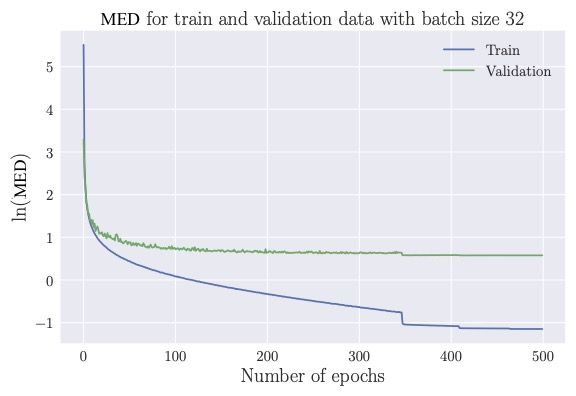
\includegraphics[width=\linewidth]{figures/Simple/new_loss.jpg}
    \caption{Training- and validation MED loss for the fully connected feed-forward (FCNN) neural network with 50,000 samples.}
    \label{fig:single_dipole_accuracy}
\end{figure}

\begin{figure}[!htb]
    \centering
    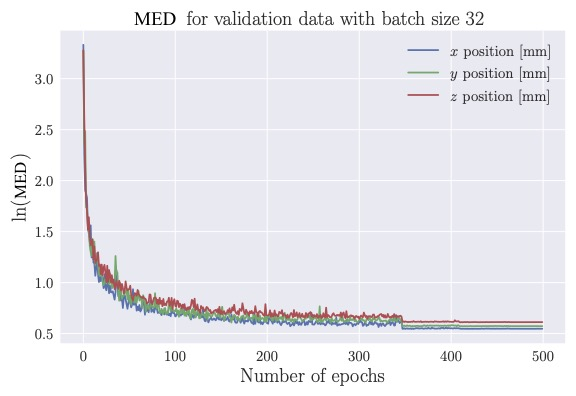
\includegraphics[width=\linewidth]{figures/Simple/new_target.jpg}
    \caption{Validation MED loss for the separate target values; the $x$-, $y$-, $z$-coordinate.}
    \label{fig:single_dipole_accuracy_targets}
\end{figure}


\subsection{Testing Methodology and Accuracy}
\rednote{Move to training chapter?}
% We begin by introducing the standard inverse problem for our neural network, DiLoc. In this context, the standard inverse problem refers to the task of predicting the x-, y-, and z-coordinates of dipole current sources responsible for generating measured EEG signals. The goal is to feed the network with EEG data corresponding to the electrical activity from randomly distributed dipoles in the cerebral cortex and have the network accurately output the locations of these current dipoles.
%For this specific problem, the network demonstrates remarkable performance even without the use of L1 regularization. However, we include L2 penalty with a value of 0.5 to promote more generalizable solutions.
Upon achieving full training convergence, a neural network demonstrates its capacity to discern essential patterns within the training data set, optimizing its parameters to minimize the cost function. To further assess the performance of the FCNN, our attention turns to an independent test data set, comprising 20,000 samples. This data set remains entirely shielded from the network during the training process, serving as an unbiased and objective gauge of the model's predictive accuracy and its ability to generalize effectively to novel, unseen data.

In order to comprehensively evaluate the neural network's performance on the untouched test data set and ensure the comparability of our results with other models, we employ a diverse set of error metrics. In addition to the primary metric of mean Euclidean distance used for assessing the accuracy of the network's predictions regarding the positions of current dipoles in the cerebral cortex, utilizing the metrics of Mean Absolute Error (MAE), Mean Squared Error (MSE) and Root Mean Squared Error (RMSE) are utilized in order to evaluating the network's performance with respect to distinct target coordinates. This approach enables us to discern whether the network faces greater challenges in predicting one dimension over others or if it consistently maintains a uniform level of performance across all coordinate dimensions.

The MAE metric provides a direct measure of the magnitude of the difference between predicted coordinates ($x$, $y$, or $z$) and their true values. MAE offers a straightforward and easily interpretable indicator of the model's prediction accuracy for each dimension. It allows us to ascertain whether the network consistently delivers precise predictions for all target values or whether variations in accuracy manifest across different coordinate dimensions.

The MSE on its side introduces a squaring process that significantly penalizes larger errors. MSE measures the variance of residuals in squared units. While this feature emphasizes and addresses substantial error spread within the predictions, it does present values in squared units of the target values. This can pose a challenge when assessing individual coordinate components.

To mitigate the squared unit issue associated with MSE while still considering error spread, RMSE is included in the evaluation framework. RMSE measures the standard deviation of residuals, balancing the emphasis on significant errors while presenting results in units that align with the target coordinate values.

Both MSE and RMSE exhibit a higher sensitivity to larger errors, as they penalize substantial deviations more strongly when calculating the average squared differences between predicted and actual values. This contrasts with the MAE metric, which treats all errors, regardless of size, on an equal footing. Consequently, a high MSE or RMSE signifies a more extensive error spread, wherein predictions substantially deviate from the true values. Conversely, a lower MSE or RMSE indicates that prediction errors are less dispersed, and most predictions closely align with the true values. Smaller MSE and RMSE values signify a superior model fit and lower prediction error.


\subsubsection{Position Spesific Performance}
The MED between the network's predictions on the unseen test data and the true target values measures 1.33 mm. It is worth noting that this error is smaller than the one observed in the validation data, mainly due to the absence of noise in the test data. This high level of precision is further exemplified by the statistics presented in Table \ref{table:MED}. All predictions for the test samples exhibit an Euclidean distance of less than 15 mm, signifying a consistently high level of accuracy. Furthermore, an impressive 99.995$\%$ of the predictions fall within an Euclidean distance of less than 10 mm, and 97.753$\%$ of the predictions achieve an Euclidean distance of less than 5 mm. This numbers indicate a notably high degree of precision.

\begin{table}[]
  \centering
\begin{tabular}{|ccc|}
\hline
\rowcolor[HTML]{CBCEFB}
\multicolumn{3}{|c|}{\cellcolor[HTML]{CBCEFB}\textbf{Euclidian Distance for Test Samples}}                                                             \\ \hline
\rowcolor[HTML]{EFEFEF}
\multicolumn{1}{|c|}{\cellcolor[HTML]{EFEFEF}ED \textless 5 mm} & \multicolumn{1}{c|}{\cellcolor[HTML]{EFEFEF}ED \textless 10 mm} & ED \textless 15 mm \\ \hline
\rowcolor[HTML]{FFFFFF}
\multicolumn{1}{|c|}{\cellcolor[HTML]{FFFFFF}99.735 $\%$}       & \multicolumn{1}{c|}{\cellcolor[HTML]{FFFFFF}99.995 $\%$}        & 100$\%$        \\ \hline
\end{tabular}
\caption{\textbf{ED between targets and predictions of test samples; Predicting Single Dipole Location with a FFNN} \newline
Performance of the network on the test data set comprising 20,000 samples, presented as the percentage of samples falling within ED thresholds of 5 mm, 10 mm and 15 mm respectively.}
\label{table:MED}
\end{table}

Table \ref{table:error_simple_dipole} displays the results for various error metrics corresponding to the network's predictions. Beginning with the MAE values for the $x$, $y$, and $z$-coordinates, we observe results ranging from 0.645 mm to 0.678 mm. These findings indicate that, on average, the network's predictions exhibit errors smaller than 1 mm in each coordinate.

The MSE values range from 0.747 mm$^2$ to 0.824 mm$^2$. The smaller MSE values signify high performance, with all values comfortably below a 1 mm$^2$ threshold. This finding indicate minimal error spread and few significant deviations between predicted and true coordinates.

RMSE values range from 0.864 mm to 0.908 mm. It is important to note that RMSE is slightly higher than the corresponding MSE values due to the square root operation involved. However, all RMSE values remain below the 1 mm threshold, signifying that the predictions maintain a limited error spread, typically staying within 1 millimeter of the actual values.

% Additionally, the $z$-coordinate's smaller representation compared to the $x$- and $y$-coordinates could contribute to the consistently larger errors in the $z$-direction.
%One plausible explanation is related to the nature of the inverse problem, where the depth of the dipole sources primarily influences the magnitude rather than the pattern of EEG recordings. However, we underscore that this discrepancy in error magnitude is very small and could also be influenced by randomness.

For an assessment of overall positional errors, the table holds the averaged Mean Absolute Error (MAE), Mean Squared Error (MSE), and Root Mean Squared Error (RMSE) across the three spatial coordinates. The resulting error values reveal minimal deviations, yielding a total MAE of 0.662 mm, a total MSE of 0.782 mm$^2$, and a total RMSE of 0.884 mm. Notably, among the three coordinates, the $z$-coordinate exhibits the highest errors accross all metrics. This observation suggests that the network might encounter somewhat greater challenges in accurately predicting the $z$-coordinate of the dipole source.

% Please add the following required packages to your document preamble:
% \usepackage[table,xcdraw]{xcolor}
% If you use beamer only pass "xcolor=table" option, i.e. \documentclass[xcolor=table]{beamer}
\begin{table}[!htb]
\begin{tabular}{l|cccc|}
\cline{2-5}
\rowcolor[HTML]{CBCEFB}
\cellcolor[HTML]{FFFFFF}                           & \multicolumn{4}{c|}{\cellcolor[HTML]{CBCEFB}{\color[HTML]{000000} \textbf{Error Metrics for Target Values}}}                                                                                                                                                                                                                                                                                                                                                     \\ \cline{2-5}
\rowcolor[HTML]{EFEFEF}
\cellcolor[HTML]{FFFFFF}\textbf{}                  & \multicolumn{1}{l|}{\cellcolor[HTML]{EFEFEF}\begin{tabular}[c]{@{}l@{}}x-coordinate\\ {[}mm{]}\end{tabular}} & \multicolumn{1}{l|}{\cellcolor[HTML]{EFEFEF}\begin{tabular}[c]{@{}l@{}}y-coordinate \\ {[}mm{]}\end{tabular}} & \multicolumn{1}{l|}{\cellcolor[HTML]{EFEFEF}\begin{tabular}[c]{@{}l@{}}z-coordinate \\ {[}mm{]}\end{tabular}} & \multicolumn{1}{l|}{\cellcolor[HTML]{EFEFEF}\begin{tabular}[c]{@{}l@{}}Position \\ Error {[}mm{]}\end{tabular}} \\ \hline
\multicolumn{1}{|l|}{\cellcolor[HTML]{EFEFEF}MAE}  & \multicolumn{1}{c|}{0.645}                                                                                  & \multicolumn{1}{c|}{0.665}                                                                                   & \multicolumn{1}{c|}{0.678}                                                                                   & 0.662                                                                                                              \\ \hline
\multicolumn{1}{|l|}{\cellcolor[HTML]{EFEFEF}MSE}  & \multicolumn{1}{c|}{0.747}                                                                                  & \multicolumn{1}{c|}{0.775}                                                                                   & \multicolumn{1}{c|}{0.824}                                                                                   & 0.782                                                                                                              \\ \hline
\multicolumn{1}{|l|}{\cellcolor[HTML]{EFEFEF}RMSE} & \multicolumn{1}{c|}{0.864}                                                                                  & \multicolumn{1}{c|}{0.880}                                                                                   & \multicolumn{1}{c|}{0.908}                                                                                   & 0.884                                                                                                              \\ \hline
\end{tabular}
\caption{\textbf{Evaluation of the FFNN performance utilizing different Error Metrics.} \newline
FFNN performance on test data set consisting of 20,000 samples. The errors are measured using Mean Squared Error (MSE), Mean Absolute Error (MAE), and Root Mean Squared Error (RMSE).}
\label{table:error_simple_dipole}
\end{table}

To further demonstrate the network's performance, we examine a randomly selected sample from the test data set. For a dipole located at x = 66.5 mm, y = -26.4 mm, and z = 41.9 mm, the network predicts the coordinates to be $\tilde{x}$ = 66.9 mm, $\tilde{y}$ = -26.1 mm, and $\tilde{z}$ = 41.7 mm. The predicted values closely align with the true values, exhibiting a minimal error of 0.4 mm in the $x$-coordinate, 0.3 mm in the $y$-coordinate, and 0.2 mm in the $z$-coordinate, resulting in a total Euclidean distance of 0.54 mm. In Figure \ref{fig:prediction_FFNN_example}, we have illustrated the network's predicted position $\mathbf{r}$ of the dipole alongside the target position $\mathbf{\tilde{r}}$.

\begin{figure}
  \hspace*{-10cm}
  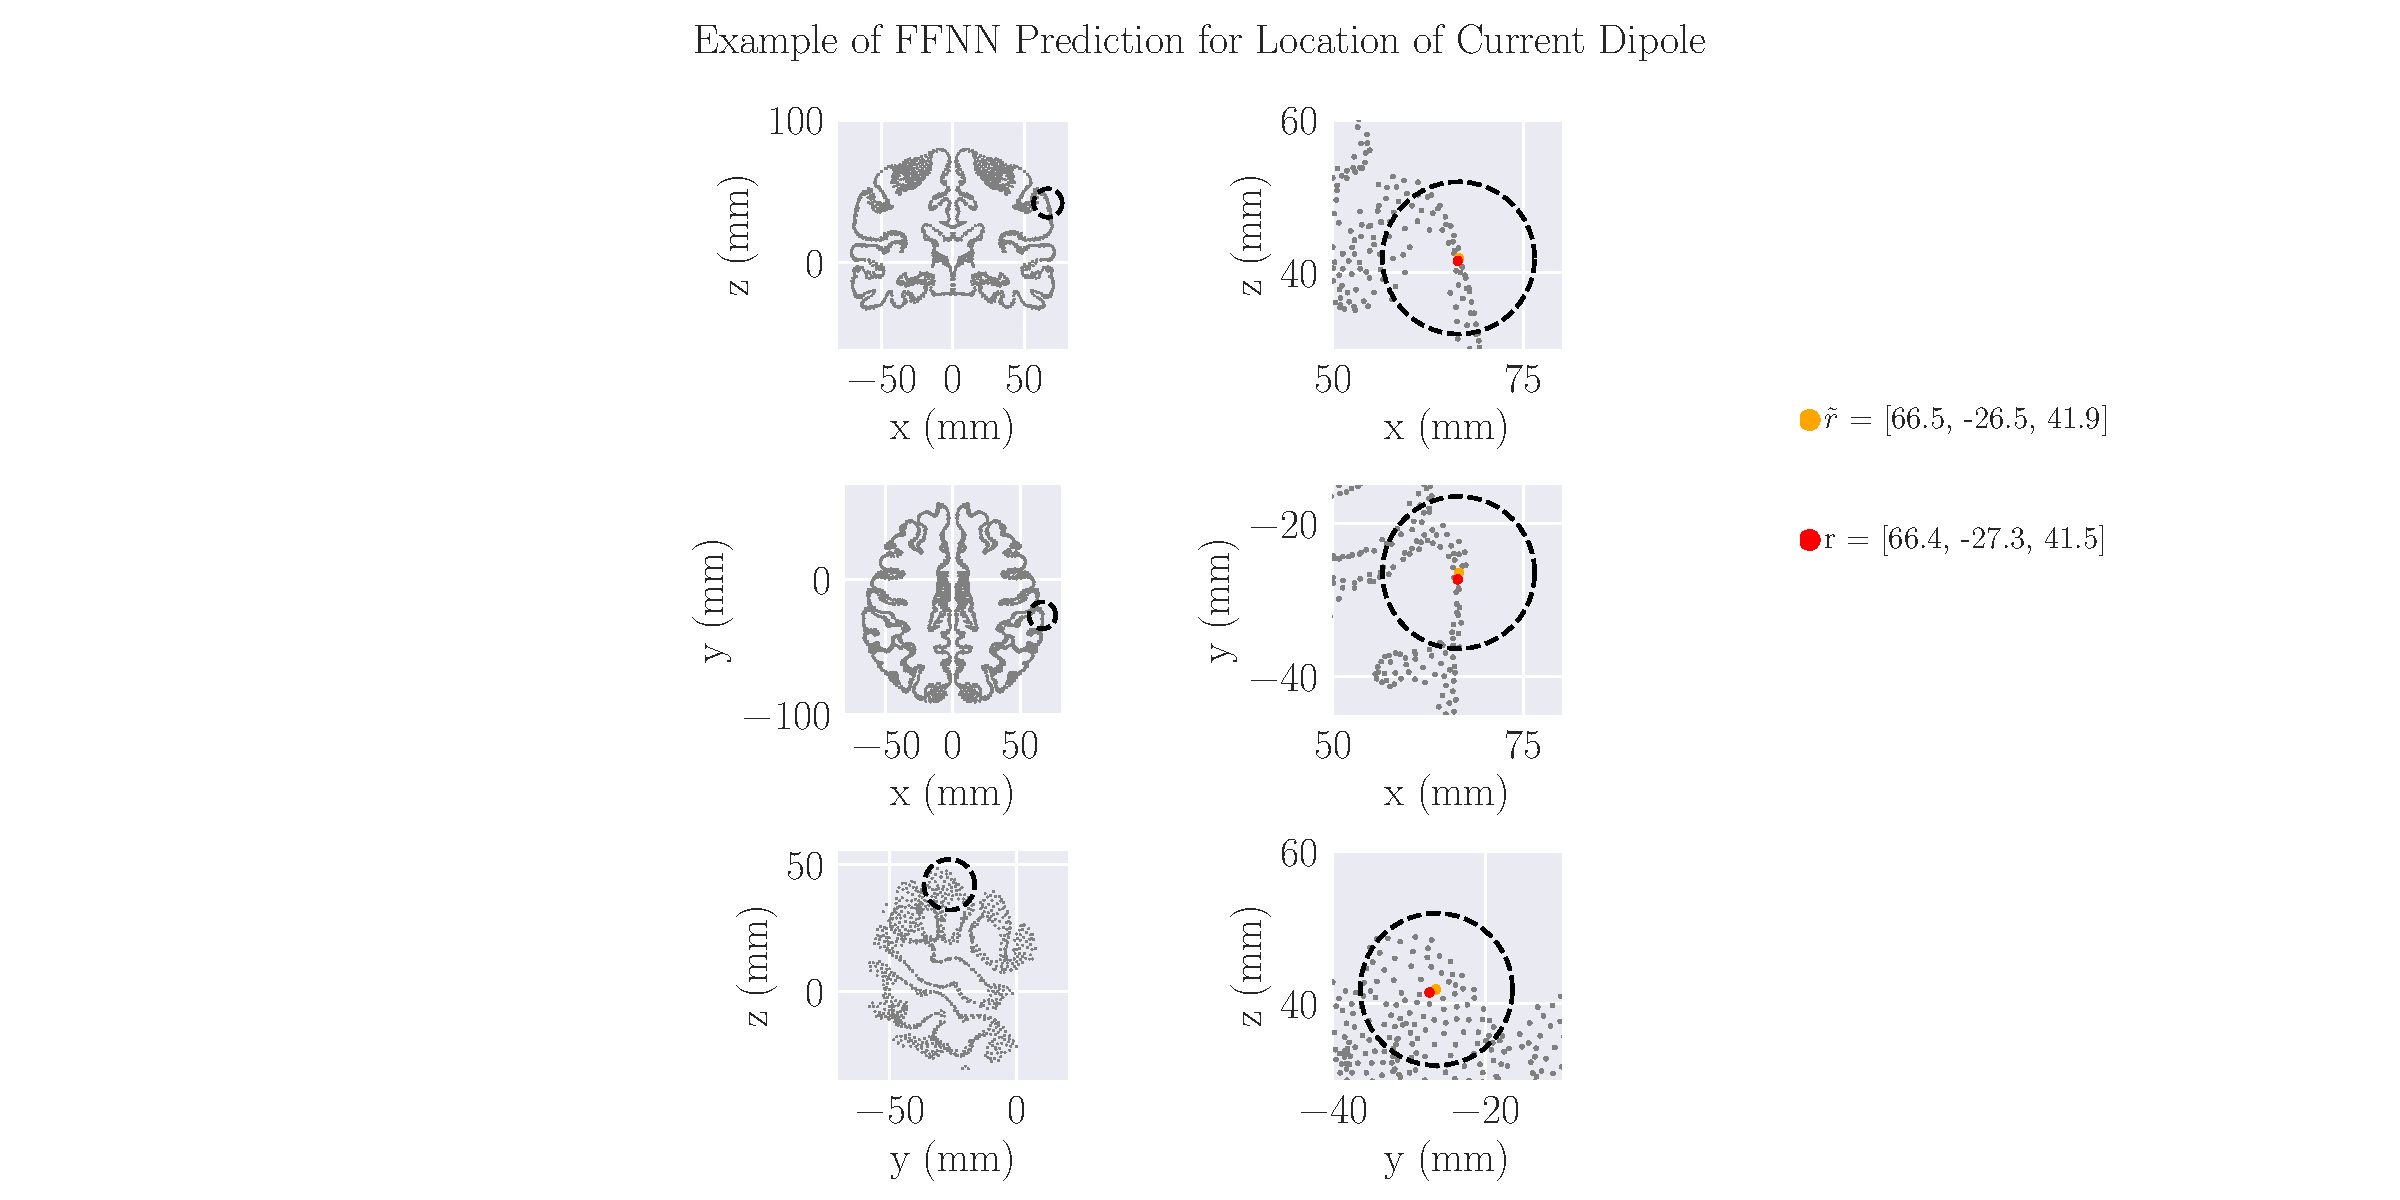
\includegraphics[width=28cm]{figures/FFNN_single_dipole_prediction.pdf}
  \caption{The networks predicted position $r$ of a dipole within the test data set and the target position $\tilde{r}$. The target dipole is marked in orange and the predicted position is marked by a red dot.}
  \label{fig:prediction_FFNN_example}
\end{figure}

\subsection{Performance at Different Brain Structures}

Figure \ref{fig:MED_crossections} presents the distribution of Euclidean Distances for various dipole locations within the New York head model cortex matrix. The figure offers valuable insights into the spread of errors across different regions of the cortex, with three cross-sections—front, top, and side—provided for examination. It is important to note that these cross-sections unavoidably include data points from the training, validation, and test data sets, making these results indicative of the network's overall performance rather than real-world scenarios. However, the analysis aims to examine the distribution of errors and identify potential areas where the network's performance may be weaker, helping to gain valuable insights into its predictive capabilities.

The Euclidean Distance (ED) values presented in the panels are mostly below 1 mm, which indicates a high level of accuracy in the network's predictions. These results are promising and demonstrate the network's ability to estimate dipole locations with a high level of precision. The panels also provide an opportunity to evaluate whether the network exhibits differential performance for dipoles located in a gyrus as opposed to those in a sulcus.

Initially, it might be assumed that EEG signals originating from dipoles in the sulcus present greater challenges for the network's analysis and prediction. This assumption is based on the deeper placement of dipoles within a sulcus compared to those in a gyrus, as well as the potential complexities introduced by the dipole's orientation within the cortex. However, upon closer examination of Figure \ref{fig:MED_crossections}, it becomes evident that the distribution of ED values does not exhibit a clear correlation with the brain's structural characteristics. The ED values seem to vary across different regions, suggesting that the network's performance is not notably affected by the differentiation between gyri and sulci. Surprisingly, the Mean Euclidean Distance for all data points where dipoles are located in a sulcus is measured to be 1.68 mm, which is even smaller than for dipoles in a gyrus, where the Mean Squared Error measures 1.70 mm. This observation further challenges the initial assumption and indicates that the network demonstrates exceptional accuracy in predicting dipole locations, irrespective of their placement within the cortex.

%These relatively small MED values further underscore the network's remarkable capacity to effectively capture the intricate features within the human brain across different cortical structures. features and variations associated with deeper cortical placements. These findings not only attest to the network's robustness but also reinforce its potential for precise dipole localization within the human brain across different cortical structures.

\rednote{Is this considered "theory" and should be mentioned earlier?}
\rednote{FIX MORE}
Further, the panels reveal a slightly higher concentration of data points with red marks in the deeper locations within the cortex, indicating higher ED values. This observation is consistent with the slightly higher error values observed for the $z$-coordinate, as presented in Table \ref{table:error_simple_dipole}, and aligns with the theory related to the nature of the inverse problem. Deep brain structures often generate weaker EEG signals, making their precise detection challenging. Hence EEG patterns for dipole sources do not cause substantial changes in the pattern of electrical potential recordings; instead, they primarily influence the magnitude of the signals, which may potentially challenge the network's ability to discriminate deep sources from each other. Said with other words, the presence of higher ED values in deeper cortical regions might be attributed to the decreasing signal-to-noise ratio of EEG signals originating from these cortical areas. With that said, we emphasize that what we here reffere to higher, red ED values, are all smaller than 15 mm, and while being somewhat larget than the mean Eucledian distance Error, they can comfortably still be considered as small errors.

In conclusion, the detailed analysis of the network's performance through cross-sectional representations provides valuable insights into its predictive capabilities. The consistently low ED across different cortical regions demonstrate the network's remarkable accuracy in estimating dipole locations. Moreover, the absence of a clear correlation between ED and brain structural characteristics suggests that the network performs robustly across diverse cortical structures.

%These results have significant implications for the network's potential clinical and research applications, as it showcases its ability to accurately predict dipole locations within the human brain, regardless of their depth and orientation within the cortex.

\begin{figure}[ht]
    \centering
    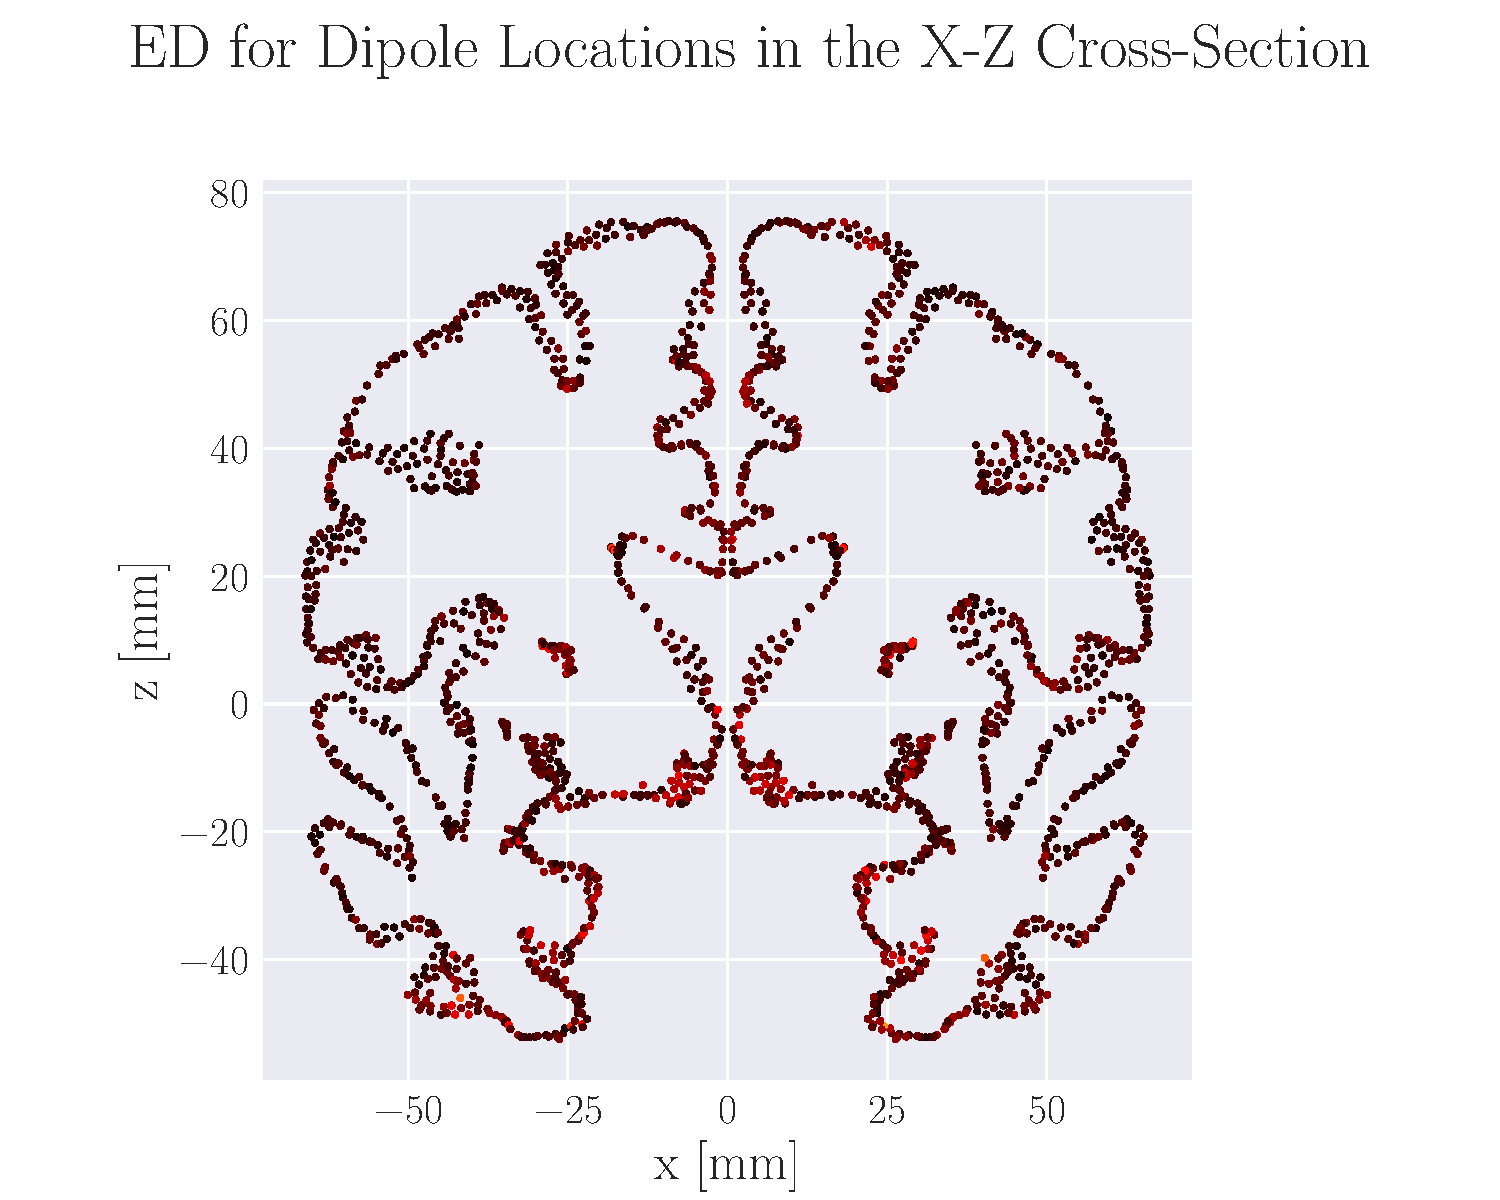
\includegraphics[width=0.7\linewidth]{figures/simple/MED_simple_dipole_error_Euclidean Distance_0.pdf}
    \vspace{10pt} % Adjust the vertical spacing between the images
    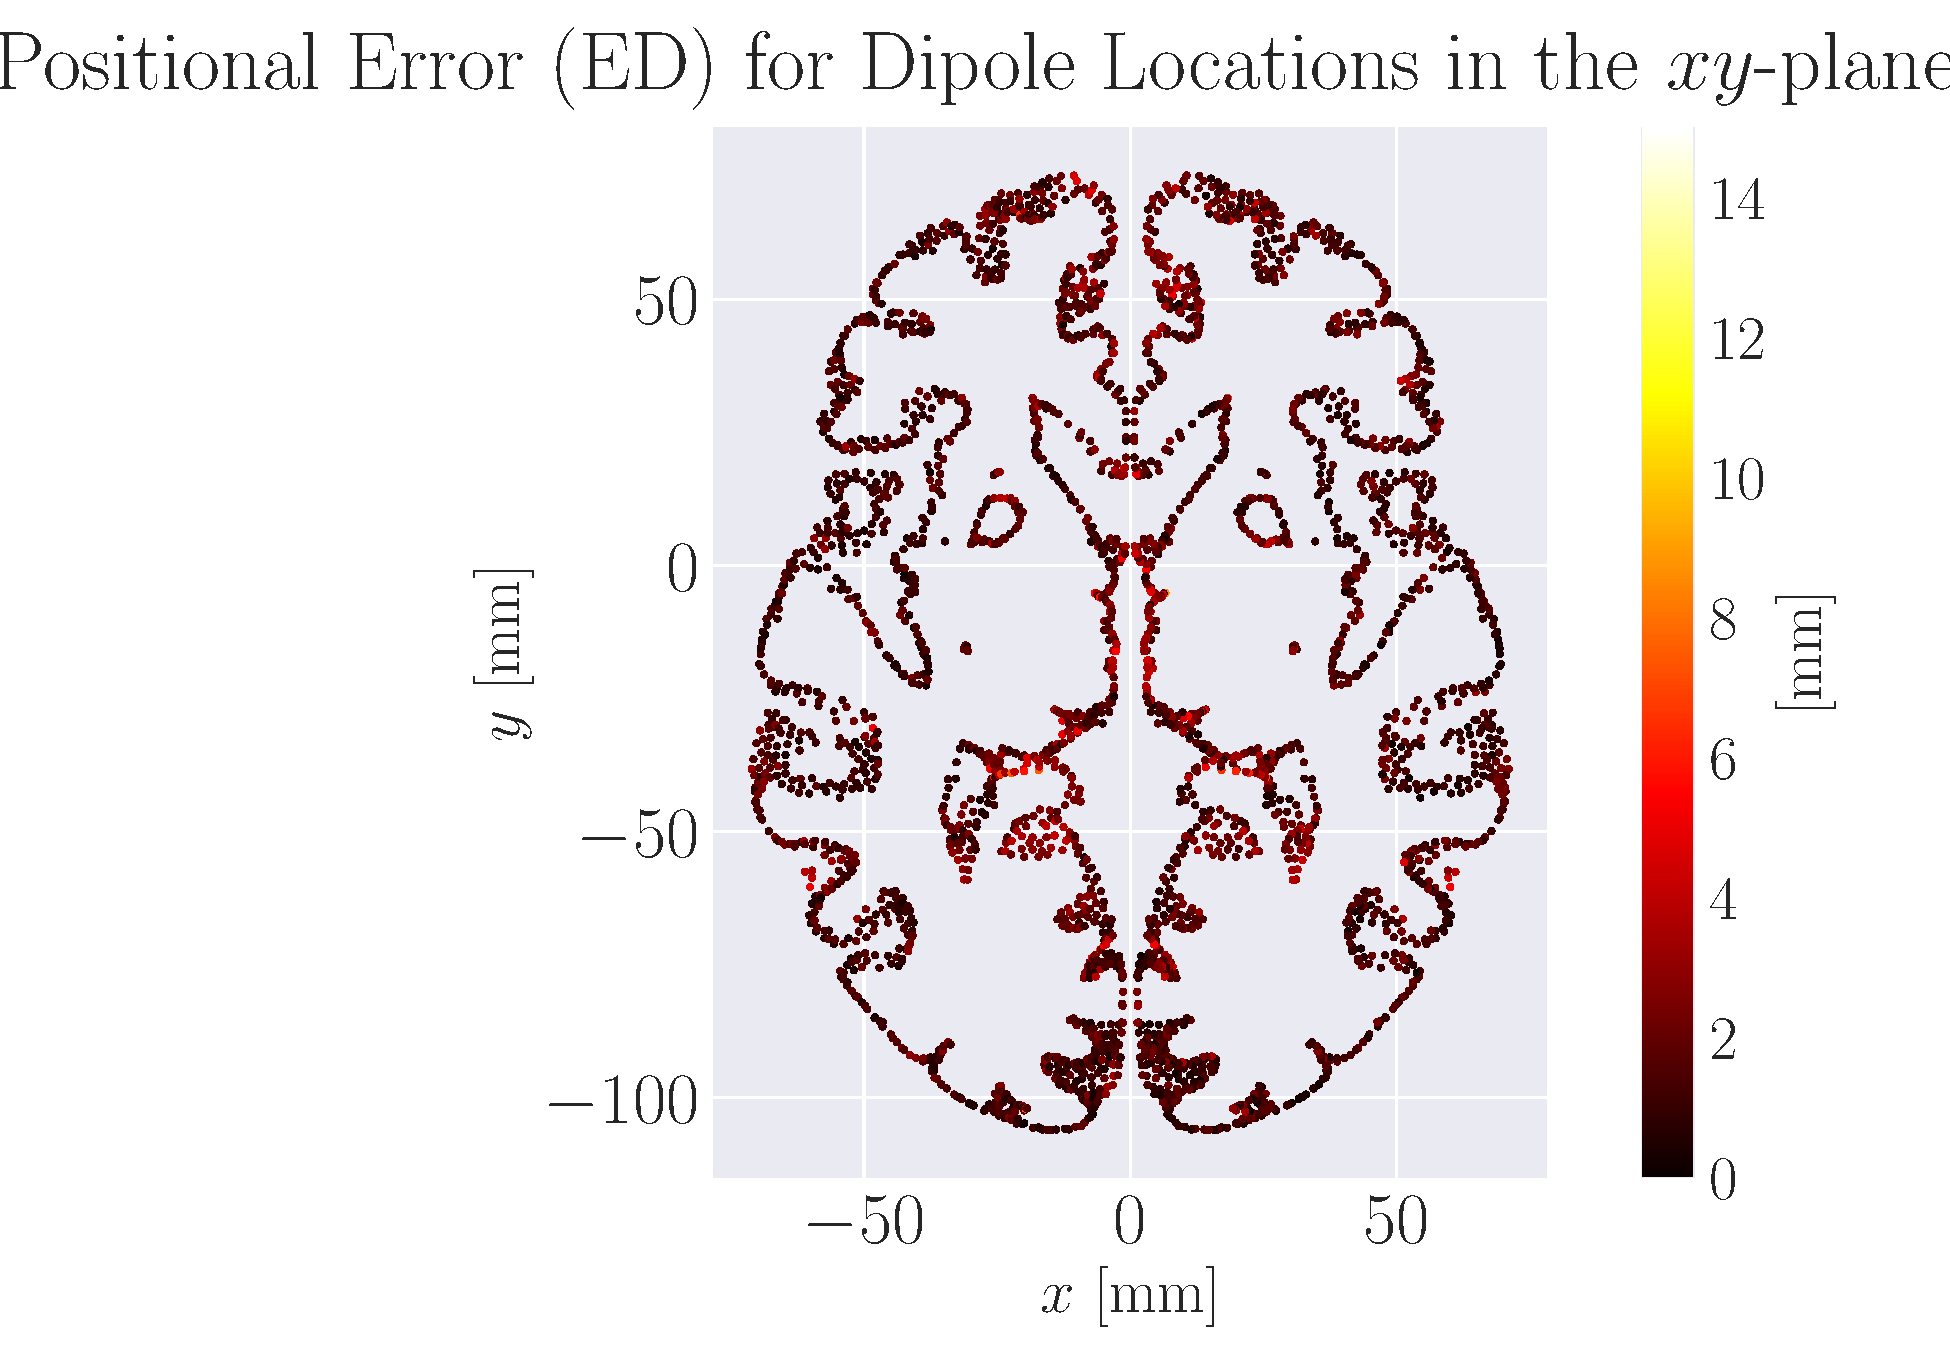
\includegraphics[width=0.7\linewidth]{figures/simple/MED_simple_dipole_error_Euclidean Distance_1.pdf}
    \vspace{10pt} % Adjust the vertical spacing between the images
    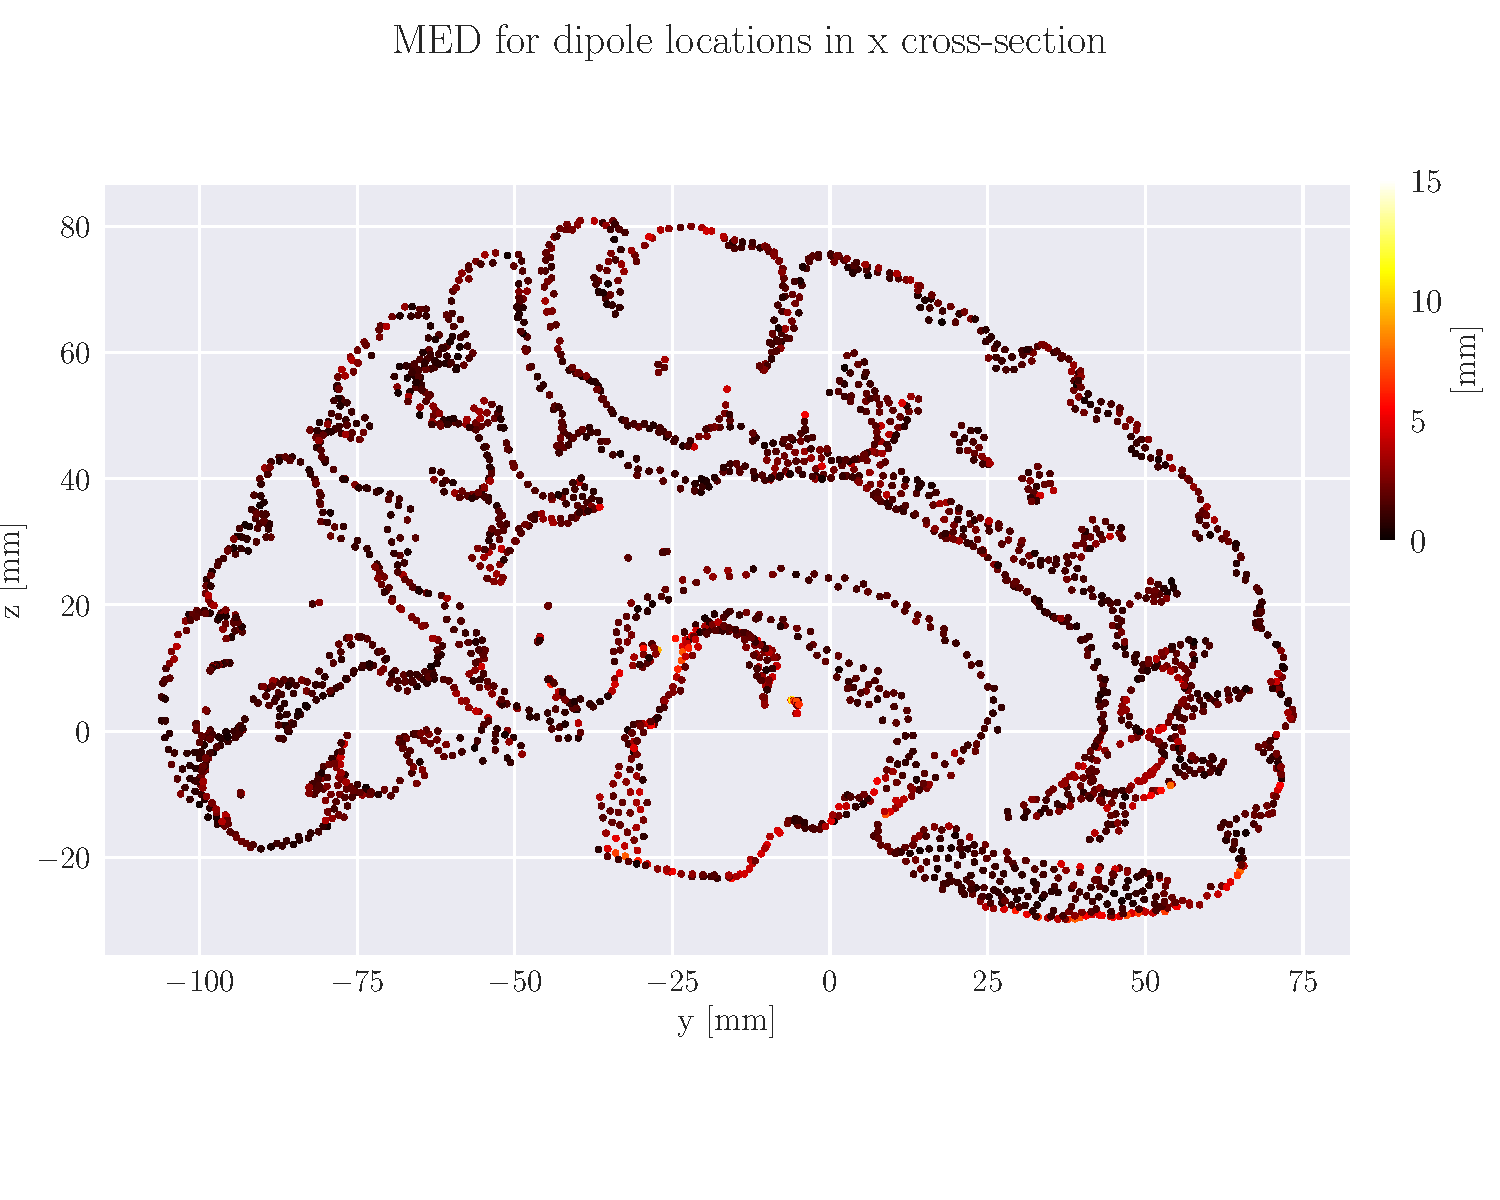
\includegraphics[width=0.7\linewidth]{figures/simple/MED_simple_dipole_error_Euclidean Distance_2.pdf}
    \caption{Different cross-sections of the cortex from the New York head model, seen from front, top and side. Each scatter point represents a possible position in the cortex matrix. The color of the fill in each circle indicates the Eucledian distance (ED) between the prediction and true value for the position of the specific dipole.}
    \label{fig:MED_crossections}
\end{figure}



\end{document}


% results extended network 
% !TEX root = main.tex
\documentclass[a4paper, UKenglish, 11pt]{uiomaster}
\usepackage{lipsum}
\usepackage[subpreambles=true]{standalone}
\usepackage[table,xcdraw]{xcolor}
\usepackage{hyperref}
\usepackage{xcolor}
\usepackage{placeins}

\begin{document}

\chapter{Extending the Fully Connected Feed-Forward Neural Network} \label{chap:extended_FCNN}
\chaptermark{Extending the FCNN}

So far we have seen how a simple FCNN and a compatible convolutional neural network performs in the task of localizing both single and multiple current dipoles. In this chapter, we will delve into how minor adjustments in data design and network architecture can enhance the FCNN's ability to identify various attributes of current dipoles. We will introduce two distinct extensions of the initial inverse problem, which will put the predictive capabilities of the FCNN to the test in handling more complex scenarios.

The first case involves extending the data set by assigning individual magnitudes to each dipole source. This extension presents the network with the task of predicting both location of the source and its corresponding magnitude. The second scenario transitions from predicting the location of a single dipole source to estimating the center and radius of a population of dipoles, while also determining the magnitude of the signal strength of the entire dipole population.

In Section \ref{sec:method}, we will outline the modifications made to the data and network architecture that have been implemented to address both of the problems. Transitioning to Sections \ref{sec:result_magnitude} and \ref{sec:result_area}, we will delve into the specifics of data simulation tailored to each problem, in addition to evaluating the network's performance when dealing with these more complex problems.

%we methodically introduce distinct modifications to the data and network architecture for each problem, assess the network's performance, and offer insights into its strengths and limitations when addressing these novel challenges.





\section{Adjusting Data Set and Architecture} \label{sec:method}
Before delving into the performance of the FCNN regarding the intricate problems of predicting dipole strength and radius alongside location, we will address important considerations that apply to both extensions. This encompasses instructing the network on how to handle varying units in its output, selecting an optimal cost function tailored to our specific problems, and establishing criteria for assessing the network's performance in the context of its intended tasks.



\subsection{Scaling of Target Values}

In the extended EEG inverse problems, the neural network is tasked with predicting target values that vary significantly in their range and units. To comprehend why this can be problematic, it is essential to revisit the purpose of the cost function. Neural networks employ cost functions to quantify the error between their predicted outputs and the target values. Depending on the cost function utilized, this error is expressed in units related to the true dimension of the target value. When a neural network has multiple outputs, the overall cost is determined by the sum of distinct errors corresponding to each output. However, adding together error terms with distinct units is a non-intuitive task. Letting the network do so, may lead to an ambiguous interpretation of the cost and hinder meaningful evaluation of the network's performance. Furthermore, the variation in the range of target values poses an additional challenge. This variation can result in certain domains of the data having an imbalanced influence on the overall error calculation, potentially overshadowing targets with smaller ranges. Such an asymmetry in the error calculation can lead to a biased optimization process and hinder the network's ability to effectively learn from the data.

To address these issues, a preprocessing step is required, which involves scaling of the target data. By instructing the neural network to output dimensionless vectors $\textbf{{y}}$ with elements constrained within the range of 0 to 1, these challenges can be mitigated.
This instruction can be given to the network by scaling the its target values
$\mathbf{\tilde{y}}_i \in \mathcal{Y}$
for $i \in \{0, N-1\}$, where $N$ is the number of samples. The scaling is done by normalizing each component of the target vector
$\tilde{\mathbf{y}_i} = [\tilde{y}_{i,0}, \tilde{y}_{i,1}, ..., \tilde{y}_{i,d-1}]$
separately. Here, $d$ denotes the dimension of $\tilde{\mathbf{y}_i}$, which corresponds to the number of target values contained in each sample. The normalized target value $\tilde{y}_{i,j}'$ for the $i$-th sample and the $j$-th dimension, is calculated as follows:
\begin{equation}
  \tilde{y}_{i,j}' = \frac{\tilde{y}_{i,j} - \text{min}(\{\tilde{\mathbf{y}}\}_j)}{\text{max}(\{\tilde{\mathbf{y}}\}_j) - \text{min}(\{\tilde{\mathbf{y}}\}_j)}.
  \label{eq:scale_target}
\end{equation}
In this equation, min($\{\tilde{\mathbf{y}}_j\}$) and max($\{\tilde{\mathbf{y}}_j\}$) represent the minimum and maximum values for a specific target dimension across all samples. By normalizing the target values in this manner, the neural network is guided to produce predictions within the range of 0 to 1. Consequently, the network's cost is computed by summing the dimensionless errors corresponding to each target prediction, for each dimension, ensuring that all target values contribute equally to the overall error calculation. As a result, the neural network learn more effectively, thereby enhancing its performance in various tasks.



\subsection{Sigmoid as Last Layer Activation Function}
In the context of predicting the position of a single dipole source, the FCNN did not employ any activation in its final layer. However, given that our output data has been normalized, we find it appropriate to use the \emph{Sigmoid} activation function in the output layer. Sigmoid is a logistic mathematical function that maps its input to a bounded range between 0 and 1, as expressed by the equation:

\begin{equation}
  f(x) = \frac{1}{1 + e^{-x}}.
\label{eq:Sigmoid}
\end{equation}

In Figure \ref{fig:sigmoid} we have provided a visualization of Sigmoid's transformation characteristics. The mapping of input values aligns with our desired output range, with normalized target values. The final layer activation aims to facilitate the training process, constraining the network from generating outputs beyond the intended normalized target range.

\begin{figure}
    \centering
    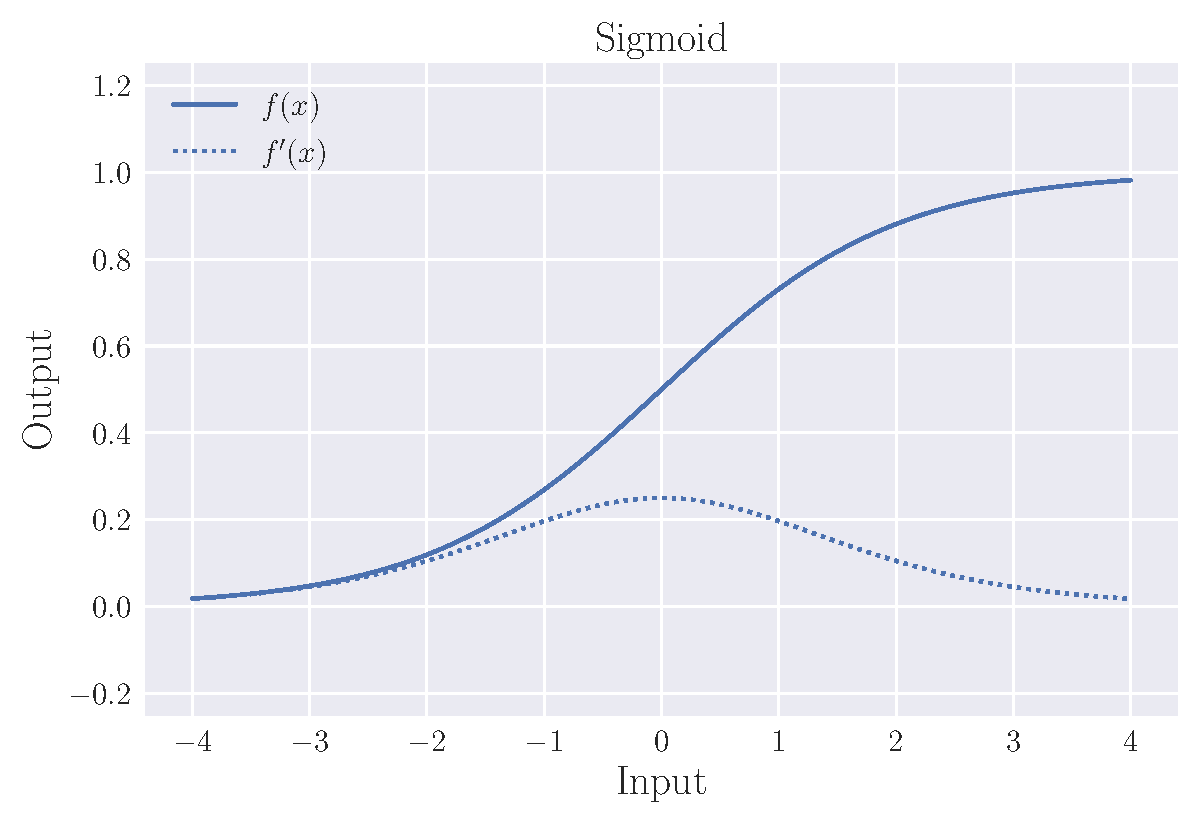
\includegraphics[width=\linewidth]{figures/Sigmoid.pdf}
    \caption{\textbf{Sigmoid activation function}: transforms the input value $x$ into a smooth S-shaped curve, mapping it to a range between 0 and 1.}
    \label{fig:sigmoid}
\end{figure}


% Include data distribution (min/max)
\subsection{Choosing an Optimal Cost Function}
The formulation of a customized cost function tailored to the specific modeling objectives is imperative when confronted with machine learning problems in need of multiple network outputs, each characterized by distinct units and interpretations, such as ours.  We aim to construct a model that can effectively predict not only the spatial coordinates of a current dipole moment but also accurately estimate the dipole's magnitude and the radii associated with a population of multiple current dipoles. To achieve this objective, our ideal cost function comprises several components.

Firstly, it calculates the Euclidean distance between predicted spatial coordinates
$x, y, z \in \mathbf{y}$
and corresponding true values
$\tilde{x}, \tilde{y}, \tilde{z} \in \mathbf{\tilde{y}}$
for $N$ number of samples:
\begin{equation}
  \text{MED}(\mathbf{y}, \mathbf{\tilde{y}}) = \frac{1}{N}\sum_{i=0}^{N-1}\sqrt{(x_{i} - \tilde{x}_{i})^2 + (y_{i} - \tilde{y}_{i})^2 + (z_{i} - \tilde{z}_{i})^2}.
\end{equation}
Additionally, the cost function calculates the absolute error between the predicted magnitude ${A} \in \mathbf{y}$ and the true magnitude $\tilde{A} \in \mathbf{\tilde{y}}$:
\begin{equation}
  \text{MAE$_A$}(\mathbf{y}, \mathbf{\tilde{y}}) = \frac{1}{N} \sum_{i=0}^{N-1} | A_{i} - \tilde{A}_{i} |.
\label{eq:MAE_A}
\end{equation}
Similarly, it aims to quantify the absolute error between the predicted radius ${\text{r}} \in \mathbf{y}$ and the true radius $\tilde{\text{r}} \in \mathbf{\tilde{y}}$:
\begin{equation}
  \text{MAE$_r$}(\mathbf{y}, \mathbf{\tilde{y}}) = \frac{1}{N} \sum_{i=0}^{N-1} | r_{i} - \tilde{r}_{i} |
\label{eq:MAE_r}
\end{equation}

With an output $\textbf{y} \in \mathcal{Y}(d)$, where $d$ represents the dimension of $\textbf{y}$ and $\mathcal{Y}(d) \subset \mathbb{R}^d$, a collective cost function, tailored for each of the distinct problem scenarios, can be defined as follows:
\begin{equation}
  C =
    \begin{cases}
      \begin{array}{l}
      \text{MED}(x,y,z),
      \end{array} & \text{if } d = 3\\
      \\
      \begin{array}{l}
      \text{MED}(x,y,z) + \text{MAE}(A)
      \end{array} & \text{if } d = 4\\
      \\
      \begin{array}{l}
      \text{MED}(x,y,z) + \text{MAE}(A) + \text{MAE}(r),
      \end{array} & \text{if } d = 5.
    \end{cases}
    % \label{eq:cost_function}
\end{equation}

In the case where $d = 3$, the simplest problem is considered, where the network predicts the coordinates of a single-point current dipole, as explored in Chapter \ref{chap:simple_dipole_FCNN} and Chapter \ref{chap:simple_dipole_CNN}. If $d = 4$, the network predicts the $x$-, $y$-, and $z$-coordinates of a single dipole, in addition to the magnitude $A$ of the signal strength. When $d = 5$, the target vector encompasses all previously mentioned values, along with the radius of a current dipole population.
%Finally, for $| \boldsymbol{\theta} |$ greater than 5, the multiple dipole problem is addressed, where the network predicts the locations for two or more point source dipoles situated at distinct positions within the cortex.



\subsection{Overview of Architecture and Hyperparameters}

Figure \ref{fig:NN_dipole_w_amplitude_architecture} presents a visualization of the architecture of the extended FCNN, which is designed to produce $d$ target values depending on the specific problem to solve. The architecture of the FCNN is equal to that employed for both the single dipole problem discussed in Chapter \ref{chap:simple_dipole_FCNN} and the multipole dipole problem examined in Chapter \ref{chap:two_dipole_FCNN}, with 231 input nodes, corresponding to the number of electrode recording measurements for one sample, and retains the same number of hidden nodes and layers.

\begin{figure}[!htb]
    \centering
    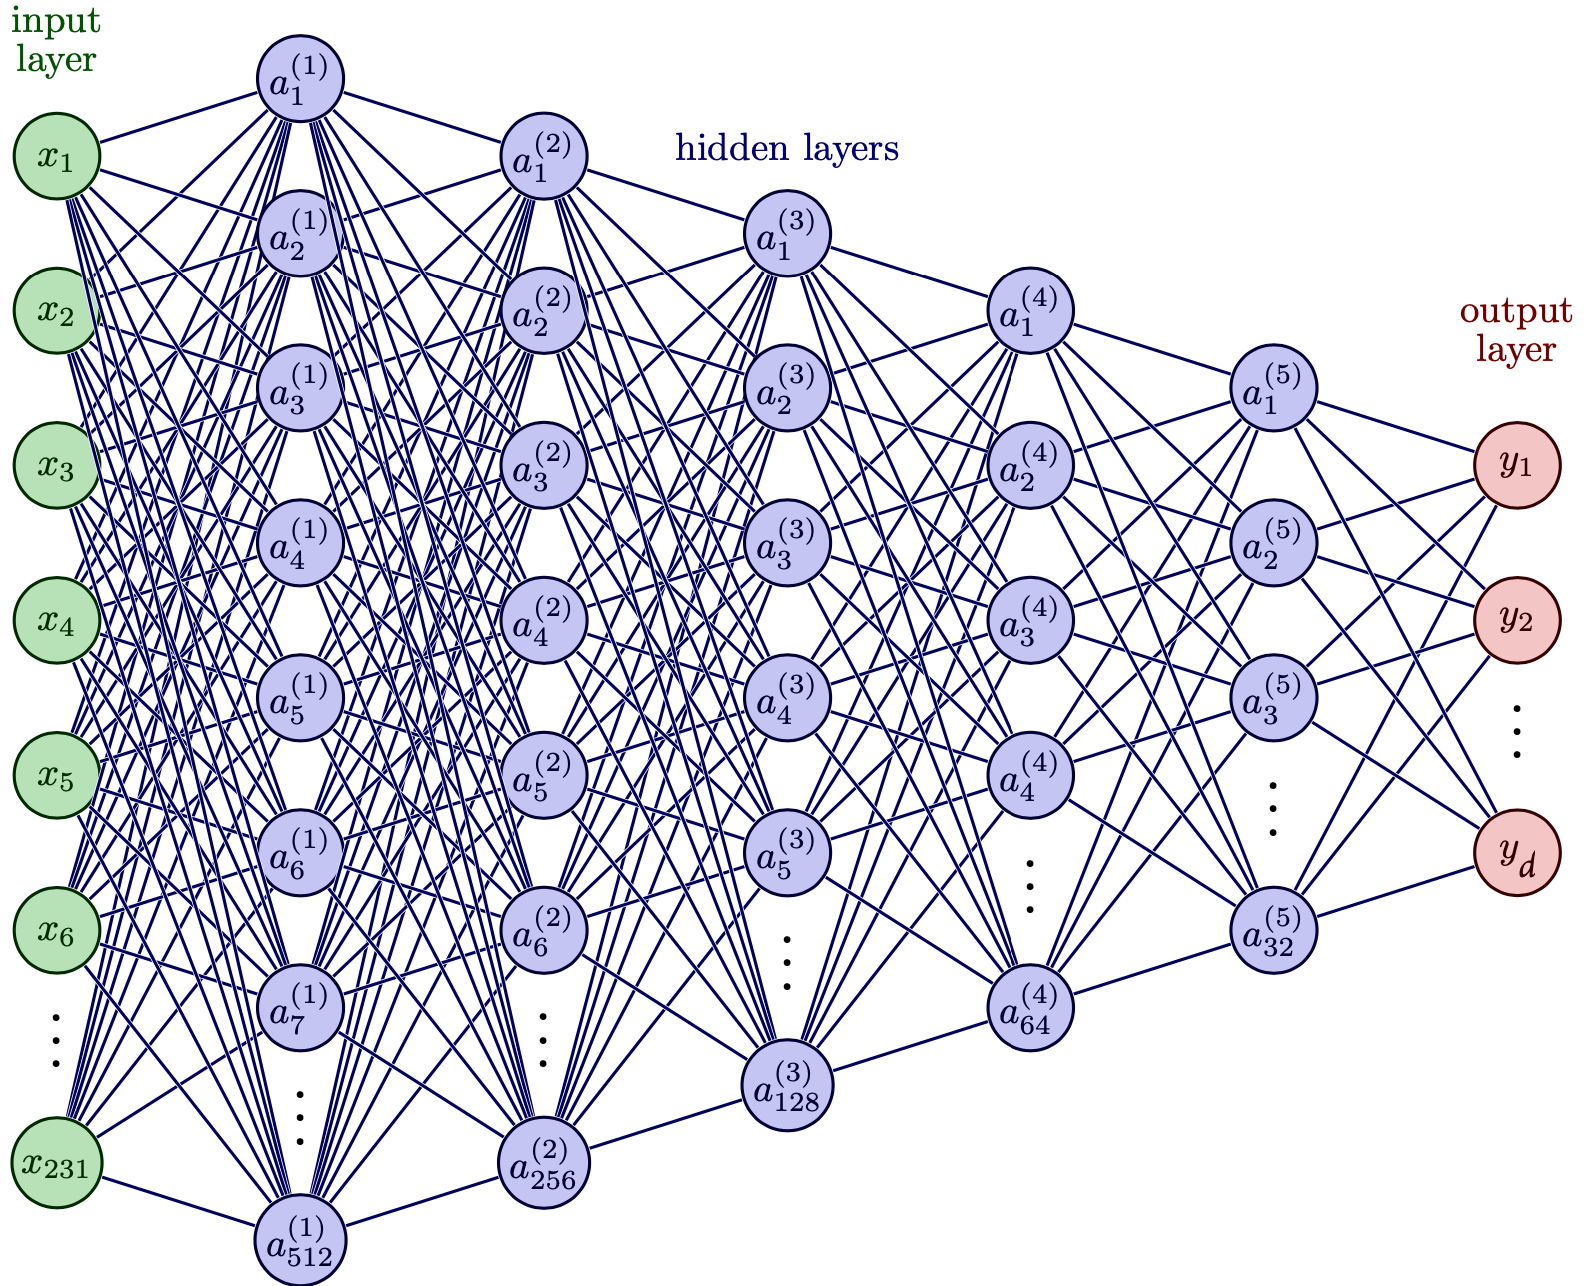
\includegraphics[width=\linewidth]{figures/NN_multiple_outputs.png}
    \caption{\textbf{Architecture of the Extended Feed-Forward Neural Network}. The input layer comprises 231 electrode recording input values, and the network outputs predicted $d$ target values depending on the specific problem to solve. The FCNN consists of five hidden layers. \\
    The visualization has been made with Latex, with code adapteded from Neural Networks in TikZ with attribution to Izaak Neutelings and is licensed under the Creative Commons Attribution-ShareAlike 4.0 International License \cite{neutelings2021}.}
    \label{fig:NN_dipole_w_amplitude_architecture}
\end{figure}

In this extension of the FCNN, we continue to employ ReLU as the activation function in the input layer and the hyperbolic tangent for the hidden layers. This choice of architecture, combined with the selected hyperparameters, has consistently yielded promising results. The key difference in this extended network architecture is the integration of the Sigmoid activation function in the output layer. For an overview of the essential hyperparameters utilized to generate the forthcoming results in this extended model, please refer to Table \ref{tab:parameters}, which offers a summary of these overall elements.


\begin{table}
\centering
\begin{tabular}{|lc|}
\hline
\rowcolor[HTML]{CBCEFB}
\multicolumn{2}{|c|}{\cellcolor[HTML]{CBCEFB}{\color[HTML]{000000} \textbf{Extended FCNN}}}    \\ \hline
\rowcolor[HTML]{EFEFEF}
\multicolumn{1}{|l|}{\cellcolor[HTML]{EFEFEF}\textbf{Hyperparameters}} & \multicolumn{1}{l|}{\cellcolor[HTML]{EFEFEF}\textbf{Value}} \\ \hline
\multicolumn{1}{|l|}{Hidden layers}                                    & 5                                                           \\ \hline
\multicolumn{1}{|l|}{Optimizer}                                        & SGD                                                         \\ \hline
\multicolumn{1}{|l|}{Learning rate (initial)}                          & 0.001                                                       \\ \hline
\multicolumn{1}{|l|}{Momentum}                                         & 0.35                                                        \\ \hline
\multicolumn{1}{|l|}{Weight decay}                                     & 0.1                                                         \\ \hline
\multicolumn{1}{|l|}{Mini-batch size}                                   & 32                                                          \\ \hline
\multicolumn{1}{|l|}{Dropout}                                          & 0.5                                                         \\ \hline
\multicolumn{1}{|l|}{Act.func in first layer}                           & ReLU                                                        \\ \hline
\multicolumn{1}{|l|}{Act.func in hidden layers}                         & Tanh                                                        \\ \hline
\multicolumn{1}{|l|}{Act.func in last layer}                           & Sigmoid                                                        \\ \hline
\end{tabular}
\caption{Hyperparameters for the Extended FCNN.}
\label{tab:parameters}
\end{table}


\rednote{This must come somewhere else?}
\subsection{Denormalization for Performance Evaluation}
In this extended version of the fully connected feed-forward neural network (FCNN), assessing network performance through standard train-validation-loss plots becomes less informative due to the normalization of target values and a more complex cost function. Reading off dimensionless loss values from plots, where the cost function value is plotted against epochs, provides little insight beyond whether the network is capable of decreasing the loss with an increasing number of training iterations.

When evaluating the network's performance on the test data set, which still comprises 20,000 samples, it is therefore essential that the predictions outputted by the FCNN undergo denormalization. This enables us to facilitate a meaningful evaluation against the true target values. The denormalization process takes a straight forward approach, where we simply do the opposite operations from the once performed during normalization \ref{eq:scale_target}. The denormalized predicted value $\tilde{y}_{i,j}$ of the network is then given as:

% \begin{equation}
% y_i = \left(x_i + \text{min}(x)\right) \left(\text{max}(x) - \text{min}(x)\right)
% \label{eq:de_scale_target}
% \end{equation}
\begin{equation}
\tilde{y}_{i,j} = \biggl(\tilde{y}_{i,j}' + \text{min}(\{\tilde{\mathbf{y}}\}_j\biggr) \biggl(\text{max}(\{\tilde{\mathbf{y}}\}_j) - \text{min}(\{\tilde{\mathbf{y}}\}_j)\biggr).
\label{eq:de_scale_target}
\end{equation}

Here, $\tilde{y}_{i,j}'$ is the normalized target value for the $i$-th sample and the $j$-th dimension of the target vector , where $i \in \{0, N-1\}$ and $j \in \{0, d-1\}$. In the equation min($\{\tilde{\mathbf{y}}_j\}$) and max($\{\tilde{\mathbf{y}}_j\}$) denotes the minimum and maximum values for the specific target dimension across all samples.

%
% To comprehensively gauge the network's predictive abilities on this test data set, we employ a diverse set of error metrics. While the primary focus is on minimizing the mean Euclidean distance of dipole positions and the absolute error for amplitude and radius, a range of other metrics are also explored for a comprehensive assessment. These metrics include mean absolute error (MAE), normalized mean absolute error considering the value range (NMAE), mean squared error (MSE), and root mean squared error (RMSE).



\sectionmark{Single Current Dipoles with Magnitudes}
\section{Predicting Single Current Dipole Sources with Varying Magnitudes} \label{sec:result_magnitude}
\sectionmark{Single Current Dipoles with Magnitudes}

In this section, we introduce the concept of various magnitudes for single current dipole sources, which adds an additional dimension to the output of the FCNN, with $d=4$. Besides predicting the coordinates of the dipoles for each sample, the network now also estimates the magnitude of the dipole signals. In real-world scenarios, it might be of interest to not only pinpoint the location generating  abnormal brain activity but also comprehend the \emph{strength} of abnormality.By incorporating magnitude prediction into the network, we gain valuable insights into the problem at hand, allowing the network to extract more detailed information about the underlying brain activity from the EEG data.


\subsection{Adjusting Data Set}
For the purpose of this extended EEG inverse problem, the data set is modified by introducing varying magnitudes to each dipole, ranging from 1 to 10 nAm. This adjustment does not impact the number of features, which corresponds to the number of electrode recordings for each sample. However, it does increase the number of target values by 1. Figure \ref{fig:dipole_w_amplitude_example} showcases two examples from the data set, where the dipole's location remains constant while the magnitude of the dipole signal varies. We observe that the shape of the EEG signal remains consistent while the strength of the EEG signal is significantly higher for the dipole with the largest initiated magnitude, as intended.

It is important to note that this data set represents the data before the standardization procedure of the input data. However, scaling the EEG data ensures that each electrode measurement is uniformly affected, maintaining consistent relative differences in magnitude between weaker and stronger dipole signals.

\begin{figure}[!htb]
    \centering
    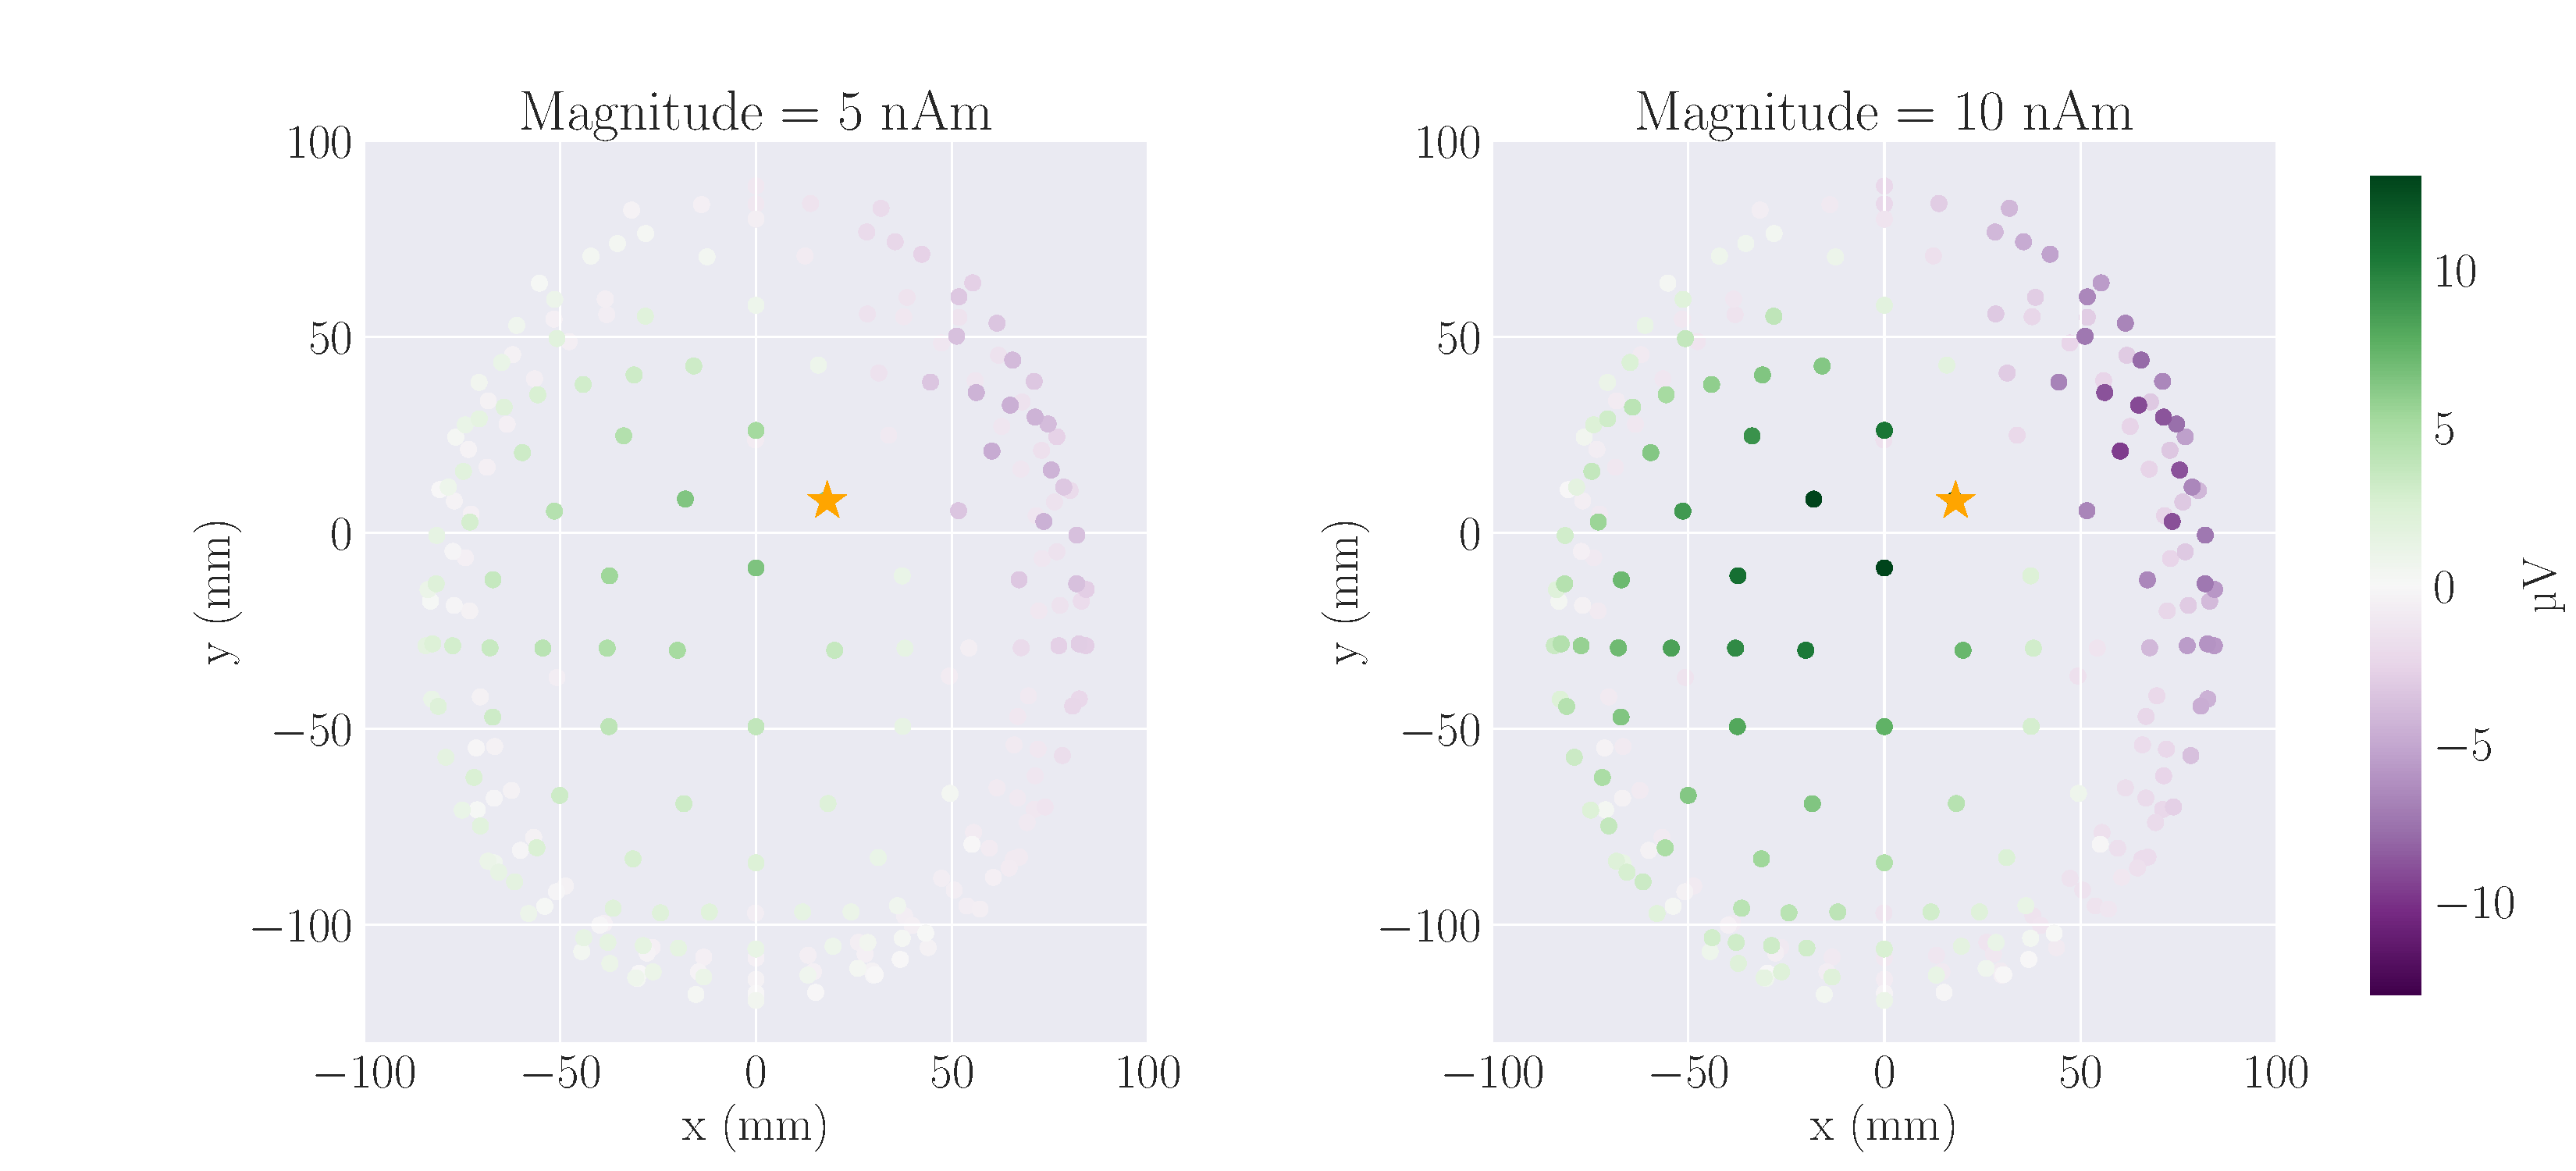
\includegraphics[width=\linewidth]{figures/purple_green/dipole_w_amplitude_example.pdf}
    \caption{EEG data for two samples with current dipole magnitudes equal to 5 and 10 nAm, respectively. The EEG recordings have a range between -10 and 10 $\mu$V.}
    \label{fig:dipole_w_amplitude_example}
\end{figure}


\subsection{Performance Evaluation}
To assess the network's performance, we start by analyzing the accuracy in relation to training epochs, as depicted in Figure \ref{fig:dipole_w_amplitude_loss}. We emphasize that it is important to note that the target values have been normalized, resulting in dimensionless loss measurements. Therefore, the figure provides a qualitative representation of the network's training progress rather than precise loss values. The plot clearly demonstrates a consistent pattern of decreasing loss as the number of epochs increases, indicating that the network is able to capture underlying patterns in the data. Moreover, both the training and validation loss stabilize after approximately 1100 epochs, suggesting that the network has reached its optimal performance level. Each epoch takes about 20 seconds to finish, leaving us with a training time of roughly 8.5 hours in total.

\begin{figure}[!htb]
    \centering
    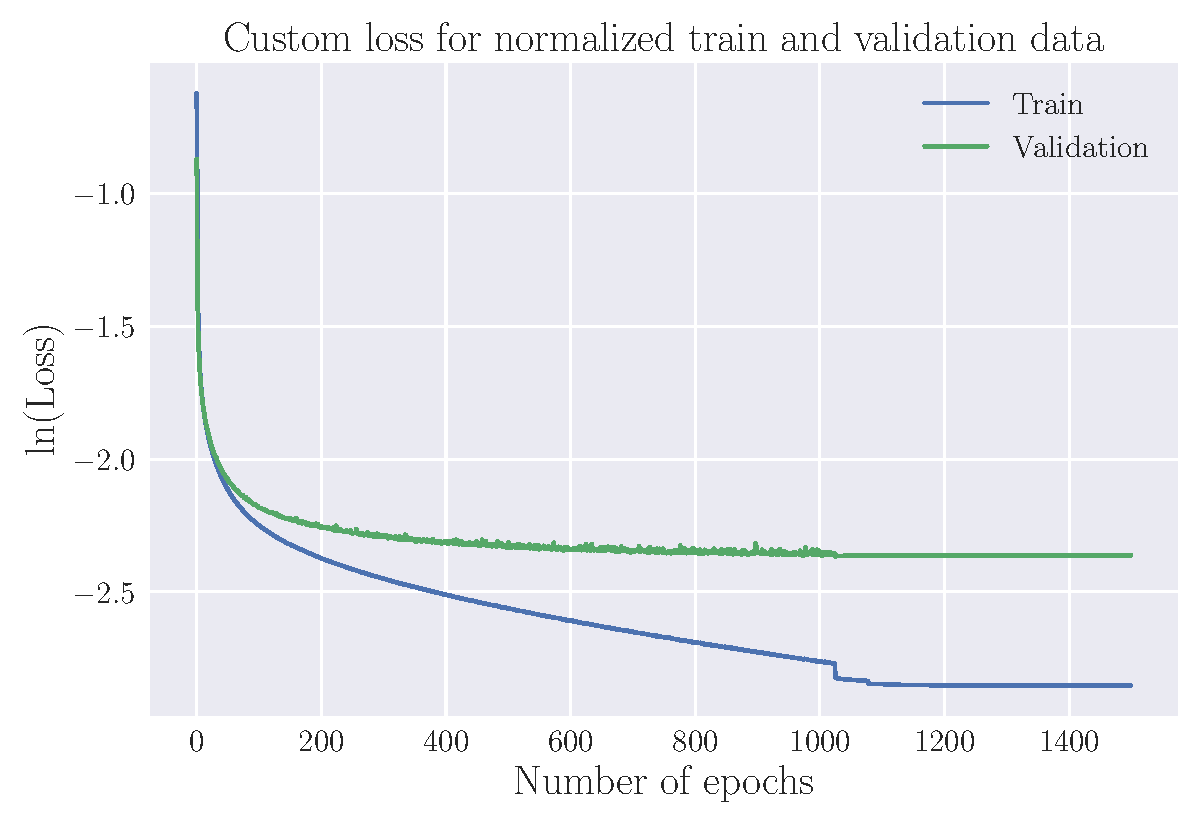
\includegraphics[width=\linewidth]{figures/NN_magnitude/Custom_Loss_amplitudes_test_custom_loss_tanh_32_0.001_0.35_0.1_0_1500_(0).pdf}
    \caption{Training and validation loss as functions of epochs for the extended FCNN model, which predicts both location and magnitude parameters. The analysis is based on simulated data comprising 50,000 samples and spans a training duration of 1500 epochs.}
    \label{fig:dipole_w_amplitude_loss}
\end{figure}

In Figure \ref{fig:dipole_w_amplitude_targets}, we present the progression of the loss for the target parameters. Notably, after approximately 1100 epochs, the loss stops fluctuating for all target values, suggesting potential full convergence at this stage. It is evident that the loss for the magnitude target converges at a higher value, compared to the target coordinates. The $x$-, $y$-, and $z$-coordinate targets gradually converge to values that closely align with one another. Among these, the $y$-coordinate achieves the lowest loss, followed by the $x$-coordinate, and then the z-coordinate.

\begin{figure}[!htb]
    \centering
    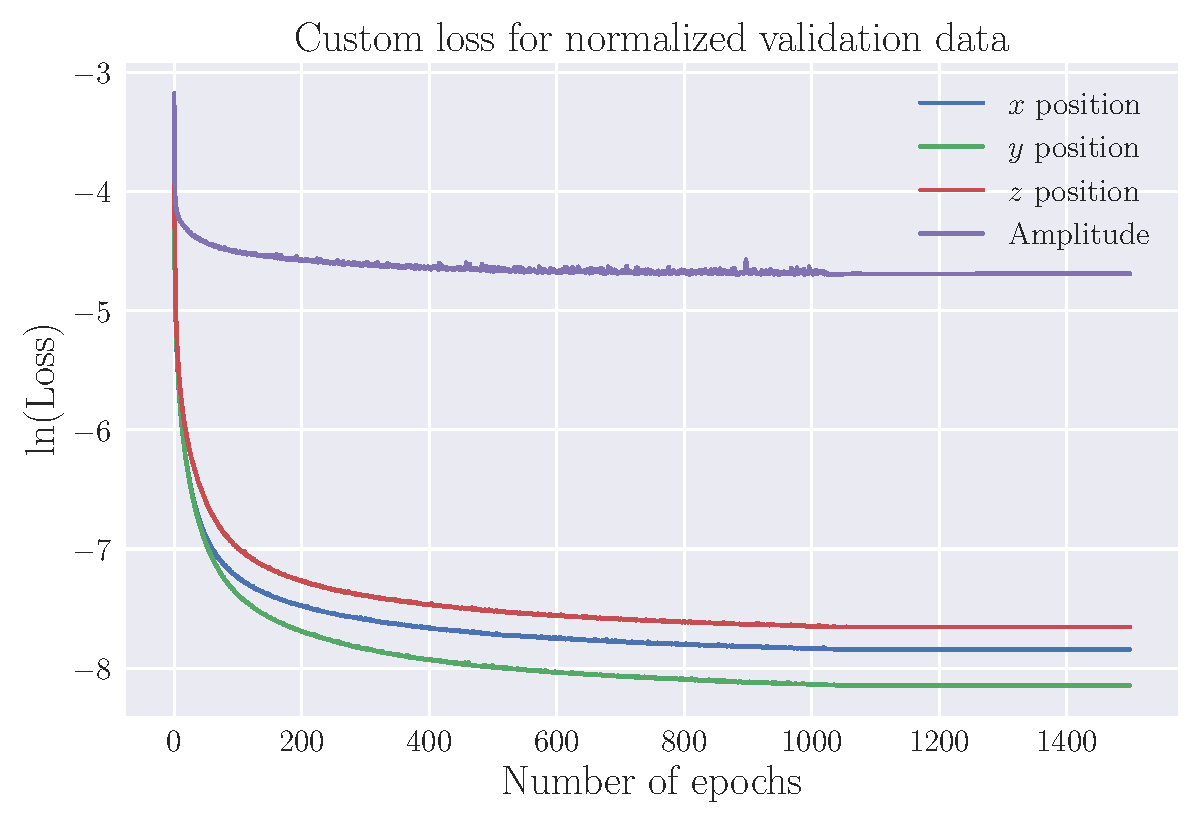
\includegraphics[width=\linewidth]{figures/NN_magnitude/Custom_Loss_mse_targets_amplitudes_test_custom_loss_tanh_32_0.001_0.35_0.1_0_1500_(0).pdf}
    \caption{Validation loss as a function of epoch for each target value, including the $x$-, $y$-, and $z$-coordinates of the dipole, as well as the magnitude of the dipole signal.}
    \label{fig:dipole_w_amplitude_targets}
\end{figure}

%Considering the range associated with each coordinate profile, we observe that the MAE for the $x$ coordinate, at 1.348 mm, accounts for only 0.936$\%$ of the complete range. Similarly, for the $y$-coordinate, exhibiting a MAE of 1.448 mm, the error relative to the coordinate range stands at 0.809$\%$. Lastly, the $z$ coordinate, with a MAE of 1.411 mm, represents 1.052$\%$ of the full range. This balanced distribution of errors suggests that no single dimension to a large extent exhibits higher error propensity than the others, thereby indicating robust overall performance. As observed in the network's performance when predicting single current dipoles with constant magnitudes, the $z$ coordinate consistently exhibits the largest error. This suggests the potential presence of specific challenges in predicting this dimension.

%MSE, due to its quadratic nature, penalizes larger errors more prominently. Despite this, the MSE values remain within reasonable bounds when contextualized within the coordinate ranges, implying a stable error profile with few significant outliers. This is a satisfying finding, especially considering the narrower range of the magnitude target. However, it is important to recognize that the theoretical lower limit of MSE is always 0, which means there is still room for further improvement in accurately capturing variations in all the target values.

%This represents a value more than 100$\%$ larger than the MED obtained when the FCNN predicted only the dipole locations for dipoles with a constant magnitude of electrical signal. Nevertheless, it is crucial to underscore that, given the dimensions of the brain within the NYHM, and the theshold value we aim to laty under, this error is relatively small and satisfactory.


In Table \ref{ch7-table:error_simple_dipole}, we present the network's performance across various target categories using different error metrics. Analyzing the outcomes pertaining to the target coordinates reveals a noteworthy consistency in mean absolute error, with an average deviation of less than 1.5 mm from the true values. In contrast to when studying single dipoles with constant strength, the $z$-coordinate stands for the highest contribution to this MAE. The MAE for the magnitude variable equals 0.539 nAm. Having that the magnitude range spans from 1 to 10 nAm, this error translates to a relative error of 6.00$\%$. In other words, the network's predictions for the magnitude variable are, on average, within 6.00$\%$ of the true values within this range.

In addition to MAE, we look into the network's performance through the metrics of mean squared error and root mean squared error, which offer complementary insights. For the $x$-coordinate, the MSE stands at 3.438 mm$^2$, while for the $y$- and $z$-coordinate, it is 3.860 mm$^2$ and 3.862 mm$^2$, respectively. The MSE for the magnitude target, measures 0.650 nA$^2$m$^2$.

The Root Mean Squared Error, which indicates the standard deviation of prediction errors and their distribution around the mean, reports values slightly lower than the corresponding Mean Squared Error values. Specifically, RMSE values measure at 1.854 mm, 1.965 mm, and 1.965 mm for the distinct target coordinates, and 0.806 nAm for the magnitude target. These RMSE values suggest that, on average, the prediction errors align with the overall spread of errors, without significant outliers or extreme deviations from the mean error. This indicates a level of stability and predictability in the error distribution.



\begin{table}[!htb]
\begin{tabular}{l|
>{\columncolor[HTML]{FFFFFF}}c
>{\columncolor[HTML]{FFFFFF}}c
>{\columncolor[HTML]{FFFFFF}}c
>{\columncolor[HTML]{FFFFFF}}c
>{\columncolor[HTML]{FFFFFF}}c |}
\cline{2-6}
                                                   & \multicolumn{5}{c|}{\cellcolor[HTML]{CBCEFB}\textbf{Error Metrics for Target Values}}                                                                                                                                                                                                                                                                                                                                                                                                                                                                                            \\ \cline{2-6}
                                                   & \multicolumn{1}{l|}{\cellcolor[HTML]{EFEFEF}\begin{tabular}[c]{@{}l@{}}x-coordinate\\ {[}mm{]}\end{tabular}} & \multicolumn{1}{l|}{\cellcolor[HTML]{EFEFEF}\begin{tabular}[c]{@{}l@{}}y-coordinate\\ {[}mm{]}\end{tabular}} & \multicolumn{1}{l|}{\cellcolor[HTML]{EFEFEF}\begin{tabular}[c]{@{}l@{}}z-coordinate\\ {[}mm{]}\end{tabular}} & \multicolumn{1}{l|}{\cellcolor[HTML]{EFEFEF}\begin{tabular}[c]{@{}l@{}}Position \\ Error {[}mm{]}\end{tabular}} & \multicolumn{1}{l|}{\cellcolor[HTML]{EFEFEF}\begin{tabular}[c]{@{}l@{}}Magnitude\\ {[}nAm{]}\end{tabular}} \\ \hline
\multicolumn{1}{|l|}{\cellcolor[HTML]{EFEFEF}MAE}  & \multicolumn{1}{c|}{\cellcolor[HTML]{FFFFFF}1.348}                                                           & \multicolumn{1}{c|}{\cellcolor[HTML]{FFFFFF}1.448}                                                           & \multicolumn{1}{c|}{\cellcolor[HTML]{FFFFFF}1.420}                                                           & \multicolumn{1}{c|}{\cellcolor[HTML]{FFFFFF}1.405}                                                                  & 0.539                                                                                                           \\ \hline
\multicolumn{1}{|l|}{\cellcolor[HTML]{EFEFEF}MSE}  & \multicolumn{1}{c|}{\cellcolor[HTML]{FFFFFF}3.438}                                                          & \multicolumn{1}{c|}{\cellcolor[HTML]{FFFFFF}3.860}                                                          & \multicolumn{1}{c|}{\cellcolor[HTML]{FFFFFF}3.862}                                                          & \multicolumn{1}{c|}{\cellcolor[HTML]{FFFFFF}3.720}                                                                 & 0.650                                                                                                           \\ \hline
\multicolumn{1}{|l|}{\cellcolor[HTML]{EFEFEF}RMSE} & \multicolumn{1}{c|}{\cellcolor[HTML]{FFFFFF}1.854}                                                           & \multicolumn{1}{c|}{\cellcolor[HTML]{FFFFFF}1.965}                                                           & \multicolumn{1}{c|}{\cellcolor[HTML]{FFFFFF}1.965}                                                           & \multicolumn{1}{c|}{\cellcolor[HTML]{FFFFFF}1.929}                                                                  & 0.806                                                                                                           \\ \hline
\end{tabular}
\caption{\textbf{Evaluation of the extended FCNN's performance utilizing different Error Metrics.} \newline
Performance for the extended FCNN on test data set consisting of 1000 samples. The errors are measured using Mean Squared Error (MSE), Mean Absolute Error (MAE), and Root Mean Squared Error (RMSE).}
\label{ch7-table:error_simple_dipole}
\end{table}

In Figure \ref{fig:magnitude_errors}, we present the AE and SE metrics calculated between predicted and target coordinate values as a function of the magnitude of the dipole strengths. The figures reveal a relatively higher occurrence of outliers when the magnitude of the dipole strength is small, with elevated AE and SE values. This trend may initially suggest that the neural network encounters greater challenges in accurately predicting the positions of dipoles with smaller magnitudes. However, we cannot rule out that these disparities might be related to alternative factors such as depth positioning or intricate cortical folding patterns.

When examining the correlation coefficients for each of the figures, we find that the correlation between the strength of the dipole and the error in position prediction has a correlation of -0.01 and -0.02 for the AE and SE, respectively. These correlation coefficients do suggest a negative correlation (decreasing error with increasing magnitudes), but their values are nearly zero, indicating a weak linear relationship. Upon closer inspection of the figure, keeping in mind that it contains 20,000 scatter points, we notice that most of the predictions exhibit an AE smaller than 5 nAm and an SE smaller than 10 nA$^2$m$^2$. This suggests that, despite observed variations in predictions for samples with smaller magnitudes, the majority of the FCNN's positional predictions consistently cluster within this range of lower errors.

\begin{figure}
  % \hspace*{-2.5cm} % Adjust the value as needed to move the figures left
  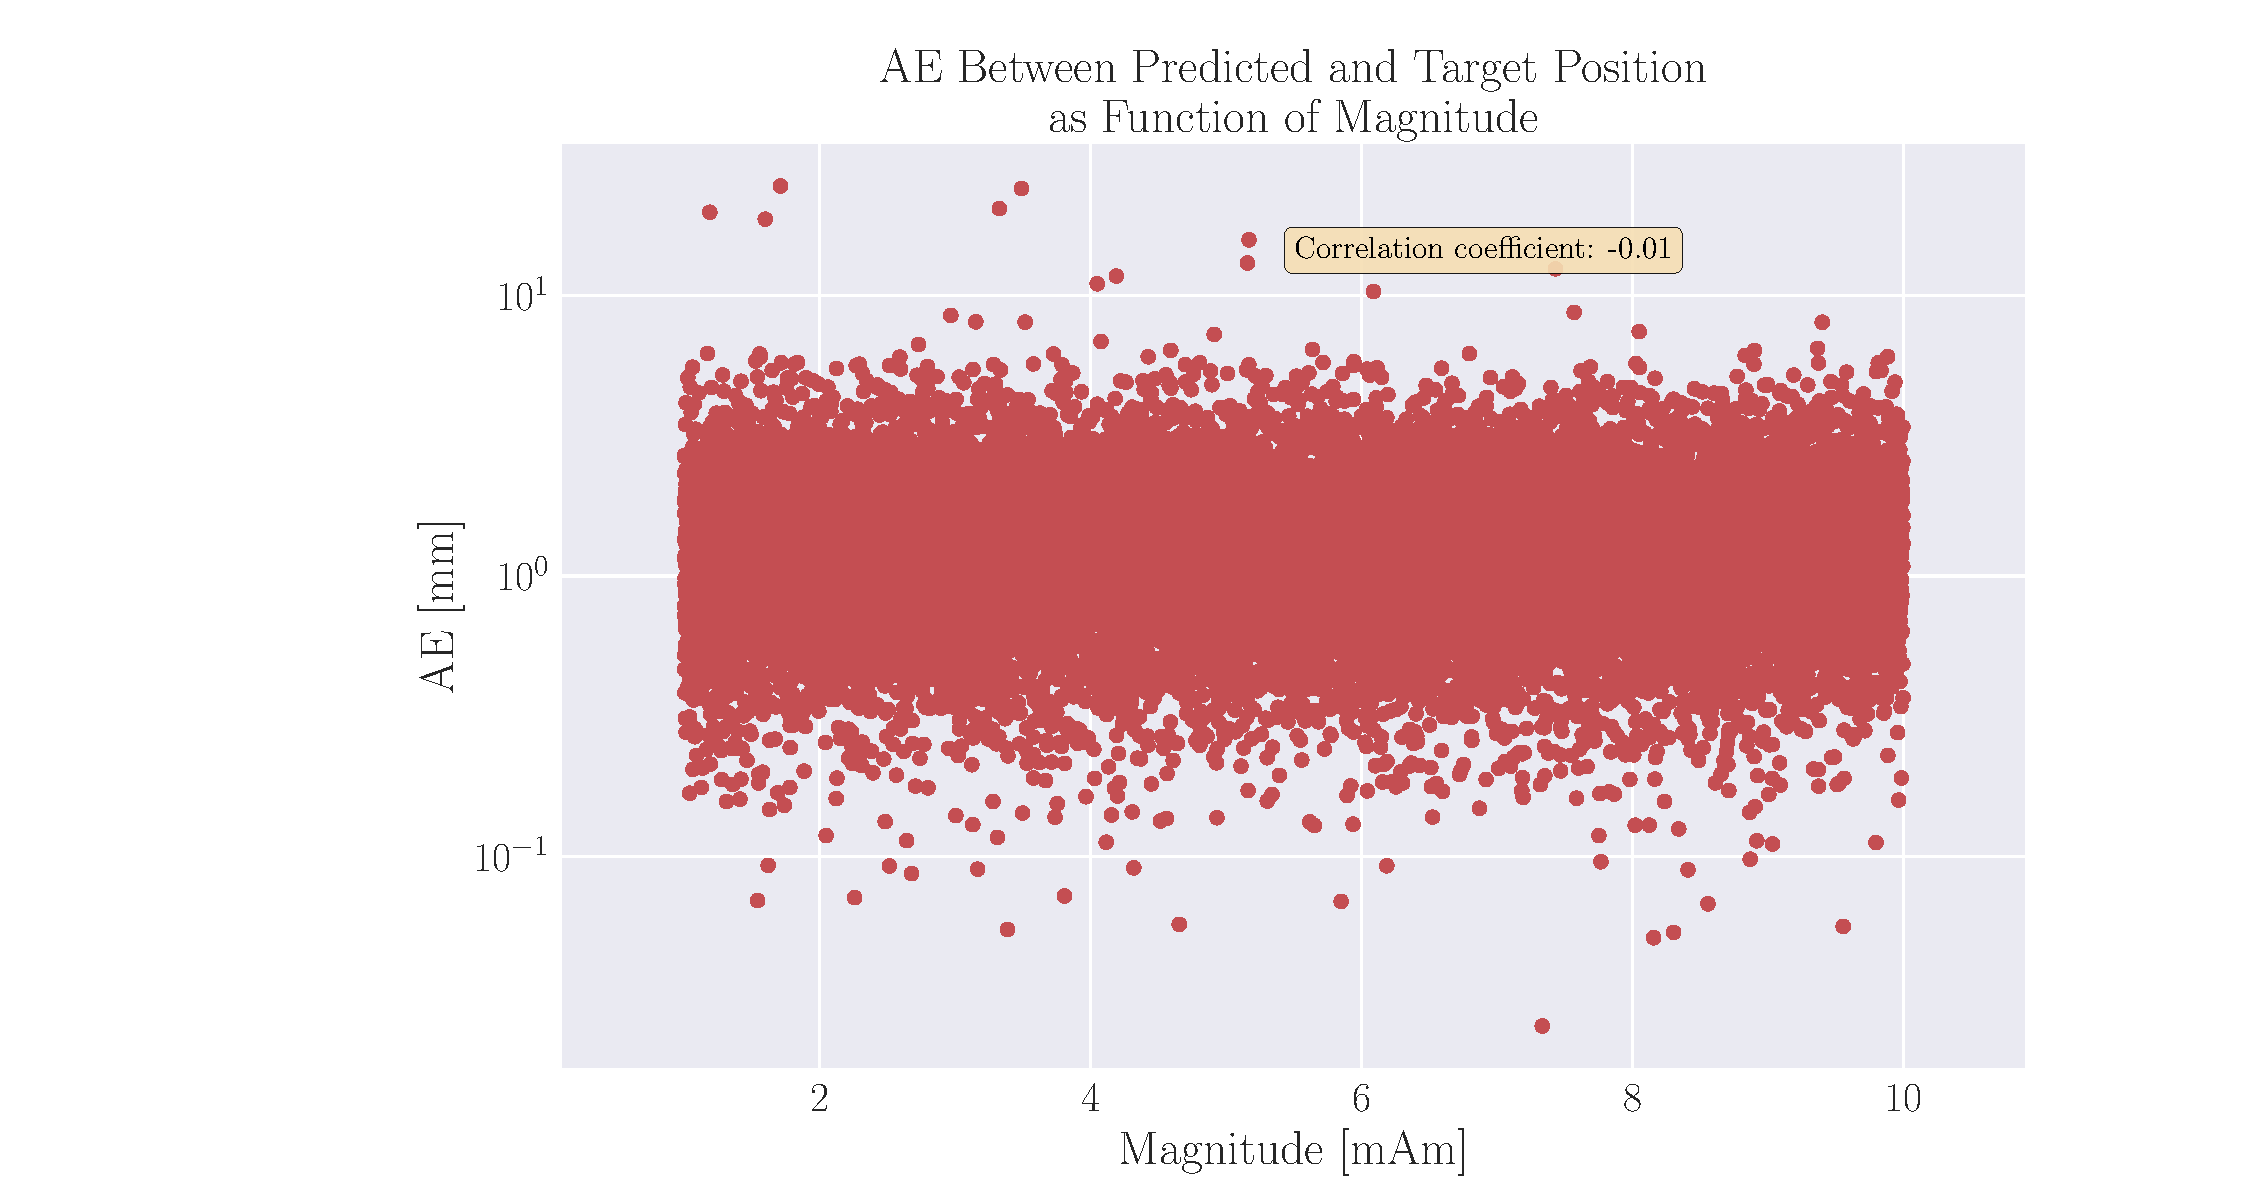
\includegraphics[width=12cm]{figures/mae_amplitude0.pdf}
  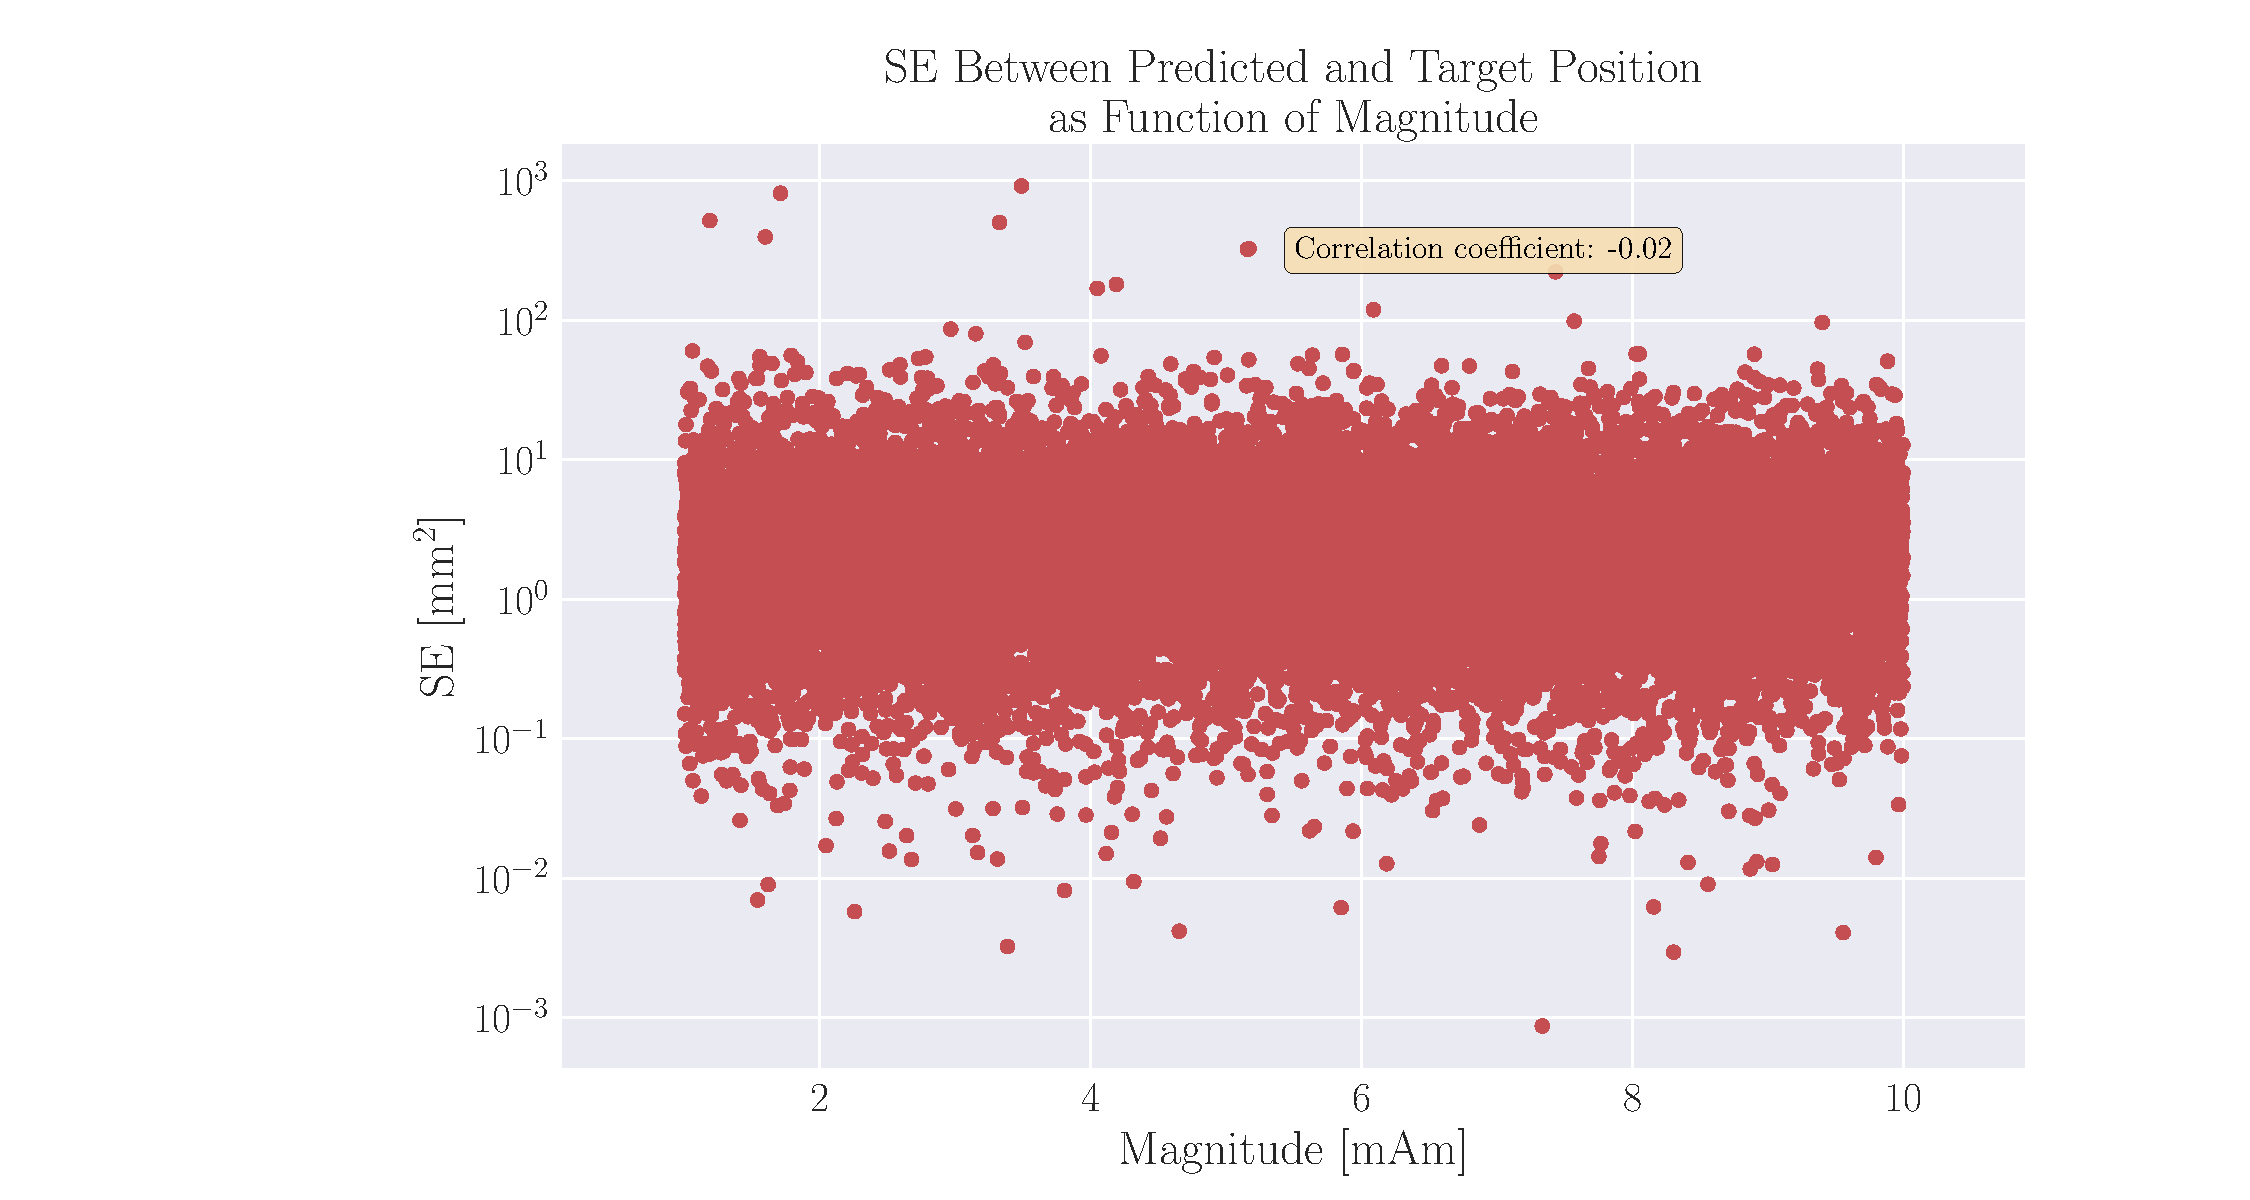
\includegraphics[width=12cm]{figures/mse_amplitude0.pdf}
  \caption{Scatter plot of Abolsute Error and Squared Error computed between predicted and target coordinate values, as function of the magnitude of the dipole strengths.}
  \label{fig:magnitude_errors}
\end{figure}

The Mean Euclidean Distance of the FCNN's predictions on the unseen test data is measured at 2.815 mm. Table \ref{table:MED_magnitude} presents the percentages of predictions of test samples falling within various MED threshold values. Notably, the network achieves an accuracy smaller than 15 mm for 99.925$\%$ of the test data. Furthermore, 90.930$\%$ of the samples exhibit a MED smaller than 5 mm, an achievement that, while robust, falls slightly short of the FCNN's performance in the previous, less complex problem.

\begin{table}[]
  \centering
\begin{tabular}{|ccc|}
\hline
\rowcolor[HTML]{CBCEFB}
\multicolumn{3}{|c|}{\cellcolor[HTML]{CBCEFB}\textbf{Euclidean Distance for Test Samples}}                                                             \\ \hline
\rowcolor[HTML]{EFEFEF}
\multicolumn{1}{|c|}{\cellcolor[HTML]{EFEFEF}ED \textless 5 mm} & \multicolumn{1}{c|}{\cellcolor[HTML]{EFEFEF}ED \textless 10 mm} & ED \textless 15 mm \\ \hline
\rowcolor[HTML]{FFFFFF}
\multicolumn{1}{|c|}{\cellcolor[HTML]{FFFFFF}90.930 $\%$}       & \multicolumn{1}{c|}{\cellcolor[HTML]{FFFFFF}99.505 $\%$}        & 99.925 $\%$        \\ \hline
\end{tabular}
\caption{\textbf{ED between targets and predictions of test samples; Predicting Location and Magnitude with the FCNN} \newline
Performance of the FCNN on the test data set comprising 20,000 samples, presented as the percentage of samples falling within ED thresholds of 5 mm, 10 mm and 15 mm respectively.}
\label{table:MED_magnitude}
\end{table}

Figure \ref{fig:histogram_magnitude} displays two panels, depicting the ED between predicted and true target coordinates and AE between predicted and true magnitude of each test sample within bins of width 1 unit. In the left panel, representing the ED histogram, the bins corresponding to ED values of 2 and 3 mm are the most populated, containing the largest proportion of samples. This panel also illustrates that the majority of predicted locations for the test samples exhibit a ED error smaller than 14 mm.

Turning our attention to the right panel, which displays the AE for predicted magnitudes, we observe that the bin holding samples with a magnitude prediction AE less than 1 nAm holds the most samples. Within this bin, 17,014 out of the 20,000 samples can be found, signifying that the network predicts the magnitude with a AE smaller than 1 nAm for approximately 85$\%$ of the sample set.

\begin{figure}
  % \hspace*{-2.8cm} % Adjust the value as needed to move the figures left
  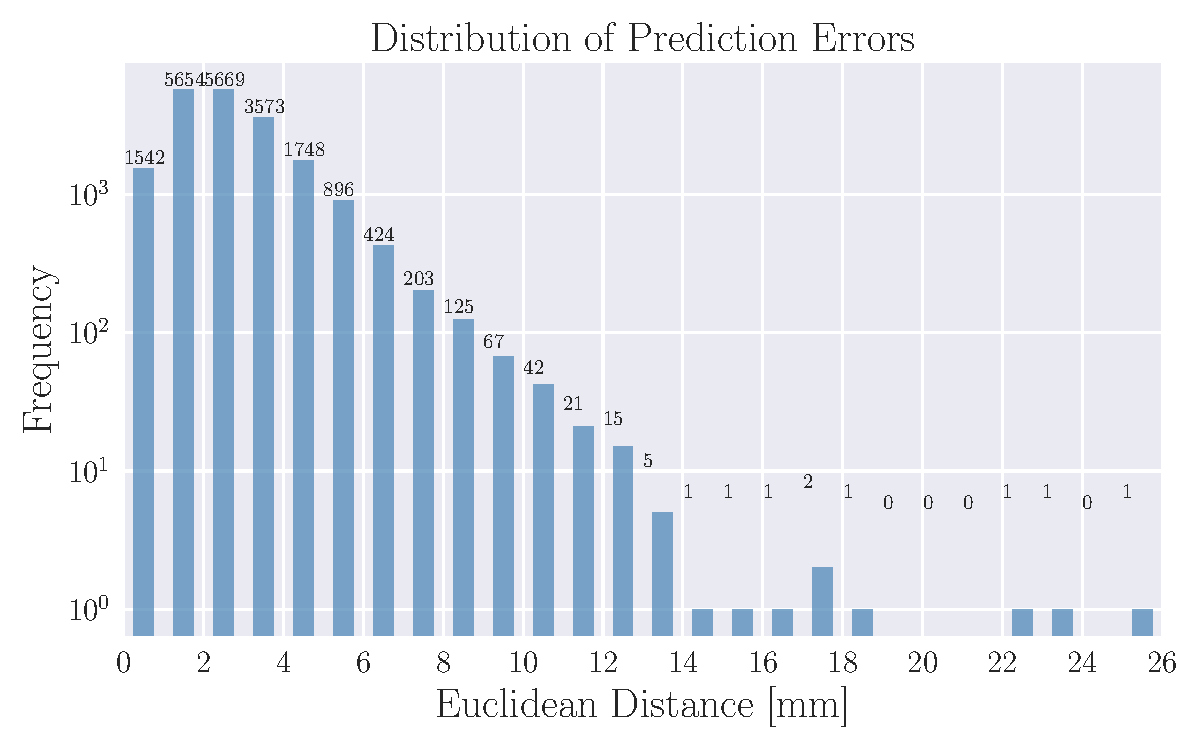
\includegraphics[width=10cm]{figures/new_histogram_position_amplitude.pdf}
  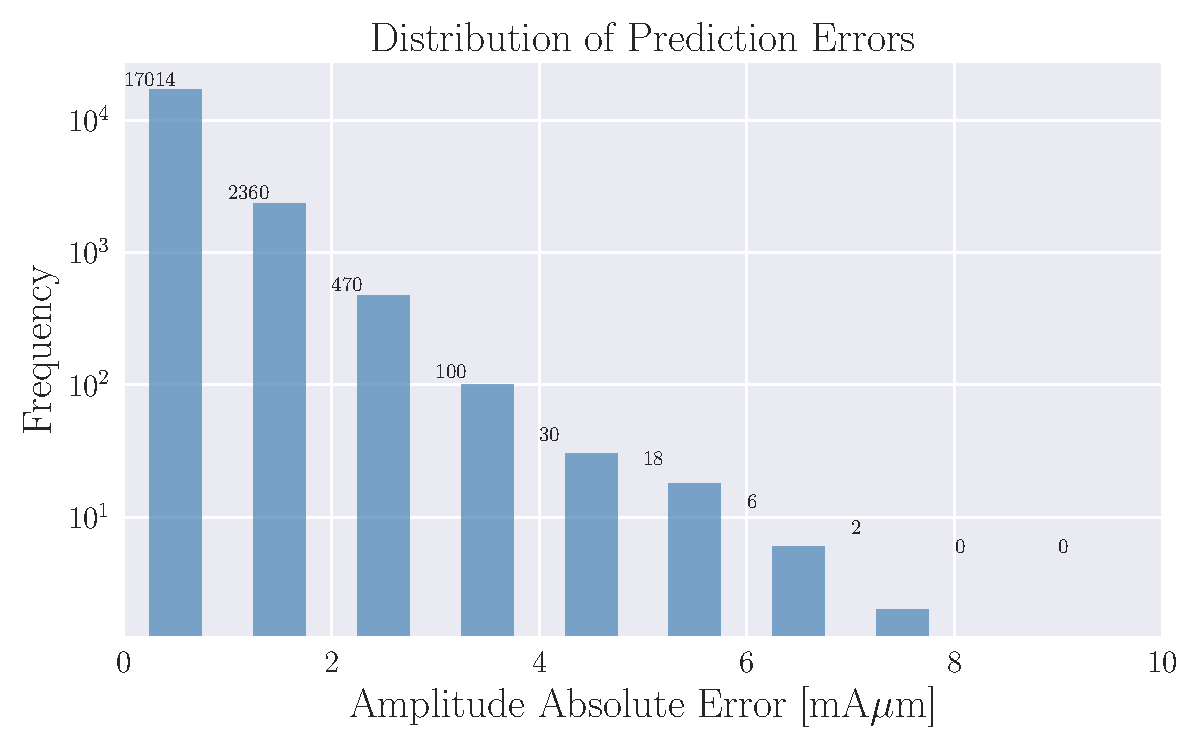
\includegraphics[width=10cm]{figures/new_histogram_amplitude_amplitude.pdf}
  \caption{Left panel illustrates the distribution of Mean Euclidean Distance for the predicted dipole locations, organized into bins of width 1 mm. Right panel holds the distribution of Mean Absolute Error for the predicted magnitude of dipole electrical signal, presented in a similar format, with bins of width 1 nAm.}
  \label{fig:histogram_magnitude}
\end{figure}



\sectionmark{Population of Dipoles with Magnitudes}
\section{Predicting Region of Active Correlated Current Dipoles with Magnitudes} \label{sec:result_area}
\sectionmark{Population of Dipoles with Magnitudes}

\rednote{Kan jeg omtale populasjonene som sfæriske?}
In this problem we expand the data set for the FCNN to include varying radii and magnitudes for the origins generating the electrical activity detected by the recording electrodes. In this extension, the FCNN progresses from predicting the location and magnitude of individual current dipole moments to estimating the centers of larger spherical populations. This enhancement aims to enable the network to extract more detailed information from EEG data, which could be valuable in scenarios where understanding the extent of brain abnormalities is crucial.

\subsection{Adjusting Data Set}
In order to optimize the neural network's capacity for predicting dipole population regions, we made specific adjustments to the data set. Within this framework, each dipole population comprises individual dipoles distributed across all points within the NY head cortex falling within a spherical volume ranging from 1 mm to 15 mm in radius. Notably, guidelines established by Delucchi et al. (1962)\cite{delucchi1962scalp}, Cooper et al. (1965)\cite{cooper1965comparison}, Ebersole (1997)\cite{ebersole1997defining}, Nunez and Srinivasan (2006)\cite{nunez2006electric}, and Schomer and Lopes da Silva (2018)\cite{niedermeyer2005electroencephalography} in the clinical context of spontaneous EEG, suggest that for EEG recordings to detect brain activity, approximately 6-10 cm$^2$ of contiguous brain tissue must exhibit synchronous activity. A spherical radius of 15 mm translates to an approximate area of 7 cm$^2$, and thus falls within this criterion \cite{nunez2019multi}.

However, when sampling event-related potentials (ERPs), which is perhaps most similar to our simulated EEG data, a different perspective emerges. In ERPs the brain's responses to specific stimuli is investigated and in order to enhance the reliability of these responses, trial-averaging is a common practice, as outlined in Chapter \ref{chap:eeg_data}. Consequently, as suggested by these authors, it becomes plausible that EEG activity arising from brain regions smaller than the typical 6-10 cm$^2$ criterion for spontaneous EEG could be detectable - population sizes that we will be training our network to identify.

% However, in the context of event-related potentials (ERPs) experiments, which is how our simulated EEG data can be considered, a different perspective arises. ERPs investigate the brain's responses to specific stimuli, and to enhance the reliability of these responses, trial-averaging is a common practice, as outlined in Chapter \ref{chap:eeg_data}. Consequently, as suggested by these authors, it becomes plausible that EEG activity arising from brain regions smaller than the typical 6-10 cm$^2$ criterion for spontaneous EEG could be detectable — population sizes that we will be training our network to identify.

For simplification reasons, we maintain the maximum amplitude strength of the total populations at 10 nAm. Consequently, we calculate the maximum number of points within a volume sphere with a radius of 15 mm and reduce this number by 10 in order to determine the strength of a distinct dipole within a given area. Having that the maximum number of dipoles that fit within a volume sphere with an ideal center and radius 15 mm was 899 dipoles, we were left with a dipole strength of 10/899 nAm for each dipole. The strength of a dipole population is thus directly proportional to the radius of the dipole population. While this may not perfectly represent real-world scenarios, it provides a reasonable approximation for our model.

In Figure \ref{fig:dipole_area}, we present an example of a dipole population and the corresponding EEG signal. The upper panels show the EEG signals for the specific sample, seen from different angels. The recording electrode locations are presented as filled circles, where the color of the fill represents the amplitude of the measured EEG signal for the given electrode. The yellow filled circles in the plots in the lower panel represents the dipole populations, i.e. positions within the cortex where dipoles have been placed. The plots within the figure are seen from the $xz$-plane, $xy$-plane, and $yz$-plane.

\begin{figure}[!htb]
\centering
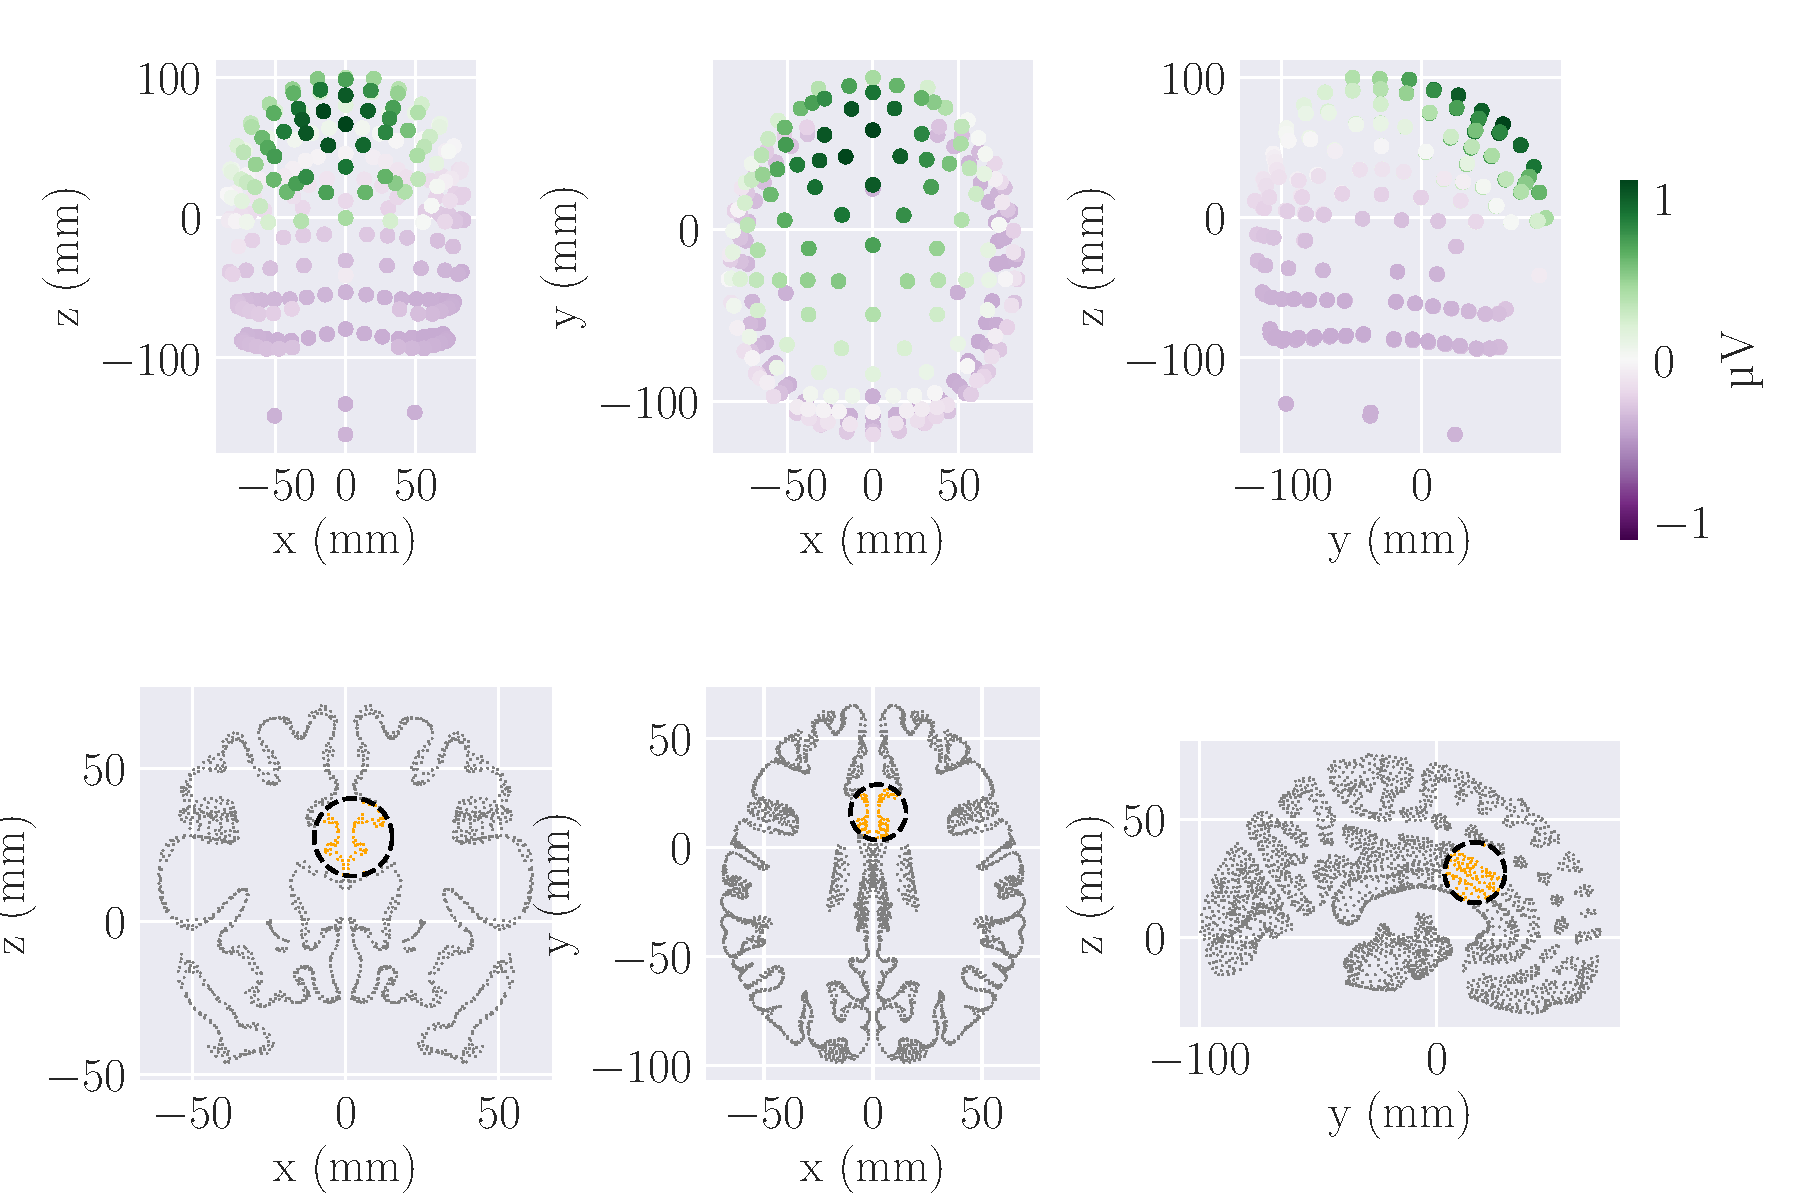
\includegraphics[width=\linewidth]{figures/purple_green/dipole_area_reduced_0.pdf}
\caption{EEG for a sample containing a spherical population of current dipole sources with a random center within the cerebral cortex.
\textbf{Upper panels:}
The EEG measure is seen from the front ($xz$-plane), side ($yz$-plane), and top ($xy$-plane) of the cortex. EEG electrode locations are presented as filled circles, where the color of the fill represents the amplitude of the measured signal for the given electrode.
\textbf{Lower panels:}
Gray filled circles represent points within the NY cortex where a dipole could have been placed. Yellow filled circles represent positions within the cortex where dipoles have been placed.}
\label{fig:dipole_area}
\end{figure}

% \rednote{Place somewhere else if needed?}
% As for the data set, the number of target values is now 5: x, y, z-coordinates of the center of the dipole population, total magnitude, and radius. The number of features within the data set is not modified and still holds 231 values, representing the EEG signal measured at every recording electrode.

% \begin{figure}[!htb]
% \centering
% 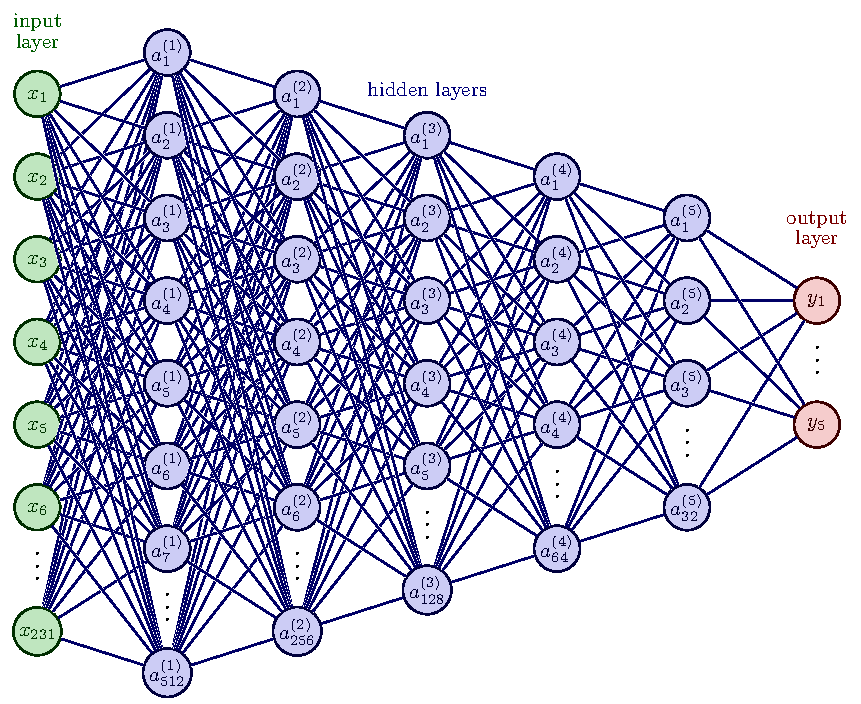
\includegraphics[width=\linewidth]{figures/NN_dipole_area_architecture.pdf}
% \caption{Architecture of the dipole area prediction network.}
% \label{fig:NN_dipole_area_architecture}
% \end{figure}

% \rednote{Rewrite/remove}
% Similar to the previous problem, we normalize the target values to ensure they all range from 0 to 1. Moreover, in this extension of the DiLoc network, we use the same activation functions as in the previous problem with ReLU as the activation function in the first layer, hyperbolic tangent for the hidden layers, and the Sigmoid activation function in the output layer.
%As with the previous problems, we have explored various network architectures and activation functions, but the current configuration has shown the best performance in terms of accurate predictions for this problem. It is important to emphasize that our primary goal is to find a network that can effectively solve the problem and provide accurate predictions, rather than necessarily seeking the best possible configuration.


\subsection{Performance Evaluation}
% How does the loss relate to size of population
% Example run and how long time it takes to calculate

In Figure \ref{fig:dipole_area_result}, we present the training and validation customized loss for the FCNN as a function of epochs. We once again emphasize that the network's loss is dimensionless, meaning that the figure only provides a visual representation of the network's training progress rather than directly interpretable loss values. The network was trained for 1000 epochs. We see a clear trend of decreasing loss with an increasing number of epochs. However, after epoch 800, both training and validation loss appears to reach convergence, and beyond this point, there is no further improvement in loss. We can therefore conclude that overfitting has not taken place during training. At epoch 749, the learning rate is adjusted from 0.001 to 0.00004, resulting in a noticeable reduction and stabilization for both training and validation loss. On average, each epoch takes approximately 23 seconds to complete, resulting in a total training time of approximately 9.5 hours.


\begin{figure}[!htb]
    \centering
    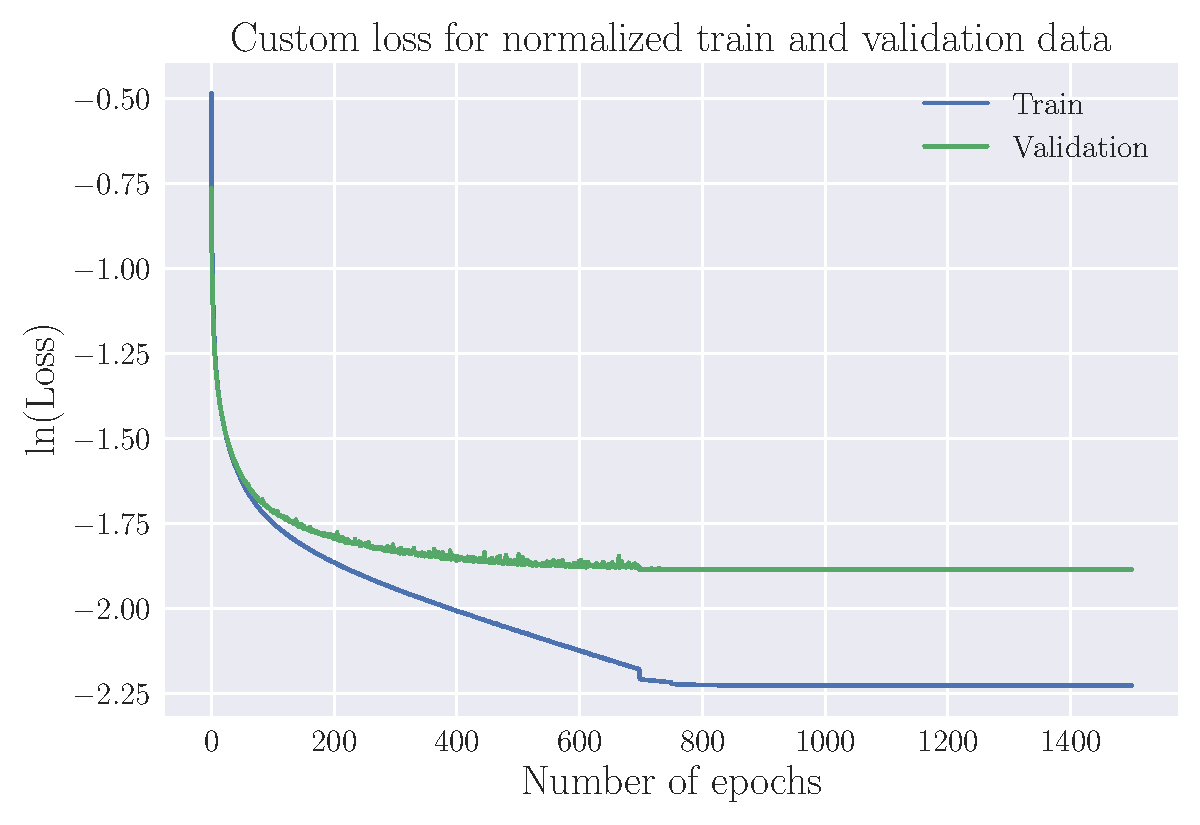
\includegraphics[width=\linewidth]{figures/NN_area/Custom_Loss_area_seed_42_cnn_32_0.001_0.35_0.1_0_1500_(0).pdf}
    \caption{Training and validation custom loss trends as functions of epochs for the FCNN model, which predicts the center, magnitude, and radius of dipole populations. The analysis is based on simulated data comprising 50,000 samples and spans a training duration of 1500 epochs.}
    \label{fig:dipole_area_result}
\end{figure}

Figure \ref{fig:dipole_area_target_result} displays the validation loss for each target value as function of epochs. We observe that the loss curves for the target coordinates reach their minima at 100 epochs and then begin to increase before stabilizing around 800 epochs. Here, the loss curves for the $x$- and $z$-coordinates are somewhat similar and stabilize at higher values than the loss for the $y$-coordinate. Shifting our focus to the magnitude and radius targets, we observe that the loss evaluations corresponding to these values follow a similar pattern. The loss curves have similar shapes, but the radius loss curve has higher losses than the magnitude curve. Somewhere between 700 and 800 epochs, these loss curves also converge. Although the loss curves for the target coordinates have their lowest values at an earlier stage, the model aims to minimize the \emph{overall} loss, and, therefore, training is not stopped at the point where the coordinate losses have their minima.

\begin{figure}[!htb]
    \centering
    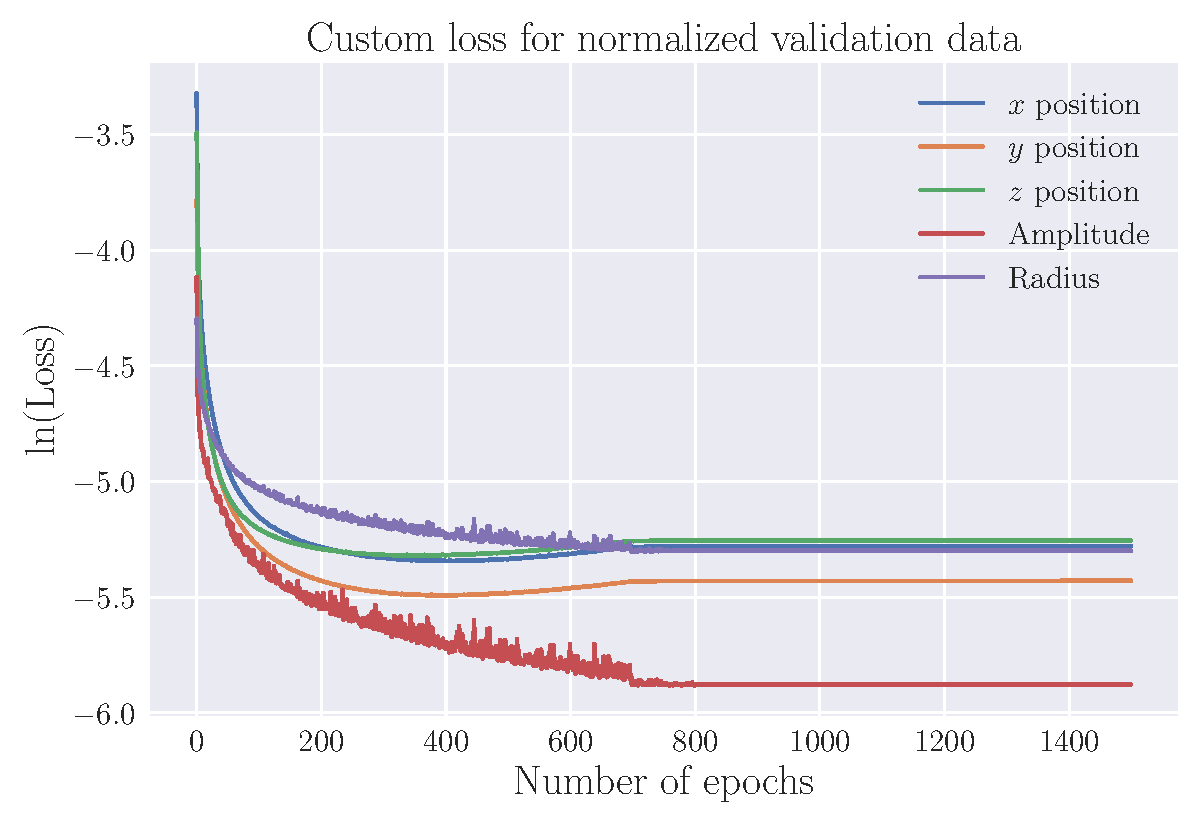
\includegraphics[width=\linewidth]{figures/NN_area/Custom_Loss_mse_targets_area_seed_42_cnn_32_0.001_0.35_0.1_0_1500_(0).pdf}
    \caption{Validation MSE loss as a function of epoch for each target value, including the $x$-, $y$-, and $z$-coordinates of the center of the dipole population, as well as the amplitude and radius.}
    \label{fig:dipole_area_target_result}
\end{figure}

\FloatBarrier


We further evaluate our model's predictions, by feeding it with unseen test data. By denormalizing the output of the network and comparing it to the target values the MED between the predicted and target coordinates measures to 7.85 mm, MAE between predicted and target magnitude equals 0.33 nAm and MAE between predicted and target radius is 0.76 mm. The MED measures a slightly higher value compared to when predicting only position and magnitude strength of the dipole. However, we note that the MAE corresponding to the magnitude has decreased in this more complex problem, now corresponding to a relative error of only 3.67$\%$. In table \ref{table:Loss_dipole_area} we can read off the percentages of the network predictions of test samples that falls within various threshold values. We have that 79.68 $\%$ of the predictions has a ED in position smaller than 10 mm, 98.57$\%$ an AE in magnitude smaller than 2 nAm and 97.22$\%$ an AE in radius smaller than 3 mm.

Table \ref{tab:thresholds_dipole_area} further provides an overview of the percentage of samples that fulfill multiple of threshold values at once. These numbers have been found with the initial condition that all predictions fulfill the constraint that the ED between predicted and target position is smaller than 10 mm. A result drawn from the table is that 78.290$\%$ of the FCNN's predictions have an AE smaller than 2 nAm in magnitude and 3 mm in radius.


\begin{table}[]
\hspace*{-2.8cm}
\begin{tabular}{|ccc|l|ccc|l|ccc|}
\cline{1-3} \cline{5-7} \cline{9-11}
\multicolumn{3}{|c|}{\cellcolor[HTML]{CBCEFB}\textbf{Euclidean Distance: Position}}                                                                                                                                                                                                                             & \textbf{}             & \multicolumn{3}{c|}{\cellcolor[HTML]{CBCEFB}\textbf{Absolute Error: Magnitude}}                                                                                                                                                                                                                             & \textbf{}             & \multicolumn{3}{c|}{\cellcolor[HTML]{CBCEFB}\textbf{Absolute Error: Radius}}                                                                                                                                                                                                                                   \\ \cline{1-3} \cline{5-7} \cline{9-11}
\multicolumn{1}{|c|}{\cellcolor[HTML]{EFEFEF}\begin{tabular}[c]{@{}c@{}}ED \\ \textless 5 mm\end{tabular}} & \multicolumn{1}{c|}{\cellcolor[HTML]{EFEFEF}\begin{tabular}[c]{@{}c@{}}ED \\ \textless 10 mm\end{tabular}} & \cellcolor[HTML]{EFEFEF}\begin{tabular}[c]{@{}c@{}}ED \\ \textless 15 mm\end{tabular} &                       & \multicolumn{1}{c|}{\cellcolor[HTML]{EFEFEF}\begin{tabular}[c]{@{}c@{}}AE \\ \textless 1 nAm\end{tabular}} & \multicolumn{1}{c|}{\cellcolor[HTML]{EFEFEF}\begin{tabular}[c]{@{}c@{}}AE\\ \textless 2 nAm\end{tabular}} & \cellcolor[HTML]{EFEFEF}\begin{tabular}[c]{@{}c@{}}AE \\ \textless 3 nAm\end{tabular} &                       & \multicolumn{1}{c|}{\cellcolor[HTML]{EFEFEF}\begin{tabular}[c]{@{}c@{}}AE \\ \textless 1 mm\end{tabular}} & \multicolumn{1}{c|}{\cellcolor[HTML]{EFEFEF}\begin{tabular}[c]{@{}c@{}}AE \\ \textless 3 mm\end{tabular}} & \cellcolor[HTML]{EFEFEF}\begin{tabular}[c]{@{}c@{}}AE \\ \textless 5 mm\end{tabular} \\ \cline{1-3} \cline{5-7} \cline{9-11}
\multicolumn{1}{|c|}{56.045$\%$}                                                                           & \multicolumn{1}{c|}{79.680$\%$}                                                                            & 86.435$\%$                                                                            & \multicolumn{1}{c|}{} & \multicolumn{1}{c|}{92.900$\%$}                                                                           & \multicolumn{1}{c|}{98.565$\%$}                                                                          & 99.685$\%$                                                                           & \multicolumn{1}{c|}{} & \multicolumn{1}{c|}{74.210$\%$}                                                                           & \multicolumn{1}{c|}{98.220$\%$}                                                                            & 99.770$\%$                                                                            \\ \cline{1-3} \cline{5-7} \cline{9-11}
\end{tabular}
\caption{Overview of network predictions of test samples falling within various threshold values.}
\label{table:Loss_dipole_area}
\end{table}

\begin{table}[]
\begin{tabular}{l|ccc|}
\cline{2-4}
& \multicolumn{3}{c|}{\cellcolor[HTML]{CBCEFB}\textbf{\begin{tabular}[c]{@{}c@{}}Predictions within different thresholds\\ (Initial condition for position: ED \textless 10 mm)\end{tabular}}} \\ \cline{2-4}
& \multicolumn{1}{l|}{\cellcolor[HTML]{EFEFEF}AE \textless 1 nAm} & \multicolumn{1}{l|}{\cellcolor[HTML]{EFEFEF}AE \textless 2 nAm} & \multicolumn{1}{l|}{\cellcolor[HTML]{EFEFEF}AE \textless 3 nAm} \\ \hline
\multicolumn{1}{|l|}{\cellcolor[HTML]{EFEFEF}AE \textless 1 mm} & \multicolumn{1}{c|}{58.075 $\%$} & \multicolumn{1}{c|}{59.940 $\%$} & 60.055 $\%$ \\ \hline
\multicolumn{1}{|l|}{\cellcolor[HTML]{EFEFEF}AE \textless 3 mm} & \multicolumn{1}{c|}{74.045 $\%$} & \multicolumn{1}{c|}{78.290 $\%$} & 78.765 $\%$ \\ \hline
\multicolumn{1}{|l|}{\cellcolor[HTML]{EFEFEF}AE \textless 5 mm} & \multicolumn{1}{c|}{74.315 $\%$} & \multicolumn{1}{c|}{78.890 $\%$} & 79.515 $\%$ \\ \hline
\end{tabular}
\caption{\textbf{Evaluation of the Extended FCNN utilizing different Error Metrics.}
Performance of the extended FCNN on a test data set consisting of 20,000 samples. The errors are measured using Mean Absolute Error (MAE), Mean Absolute Percentage Error (MAPE), Mean Squared Error (MSE), and Root Mean Squared Error (RMSE) for various target values.}
\label{tab:thresholds_dipole_area}
\end{table}

To ensure the model's accuracy is comparable to the work done by others and to further assess its ability to predict the center of dipole populations, in addition to magnitude and radius, we employ the same evaluation metrics as in previous problems: MAE, MSE, and RMSE. The results for these error metrics are presented in Table \ref{table:error_dipole_area}.

The MAEs for the target coordinates, i.e., the center of the dipole population, average at 3.96 mm. This is the highest MAE measured among the predictions made by the network across all the problems studied. As observed when predicting both the magnitude and position in the previous problem, the $z$-coordinate contributes the most to this MAE.

Concerning the MSE, we observe relatively small errors for amplitude and radius, with values of 0.312 and 1.114 mm$^2$, respectively. The MSE between the predicted and target coordinates ranges from 42.58 mm$^2$ to 66.816 mm$^2$, indicating the widest spread of errors compared to the previous problems studied. An increase in RMSE is also evident. This suggests that, on average, the prediction errors do not always align with the overall spread of errors. In other words, the model sometimes provides accurate predictions, while in other cases, it does not. This indicates a lower level of stability and predictability in the error distribution compared to the other problems studied.



\begin{table}
\begin{tabular}{c|
>{\columncolor[HTML]{FFFFFF}}c
>{\columncolor[HTML]{FFFFFF}}c
>{\columncolor[HTML]{FFFFFF}}c
>{\columncolor[HTML]{FFFFFF}}c
>{\columncolor[HTML]{FFFFFF}}c
>{\columncolor[HTML]{FFFFFF}}c |}
\cline{2-7}
\multicolumn{1}{l|}{} & \multicolumn{6}{c|}{\cellcolor[HTML]{CBCEFB}\textbf{Error for different target values}} \\ \cline{2-7}
\multicolumn{1}{l|}{} & \multicolumn{1}{c|}{\cellcolor[HTML]{EFEFEF}\begin{tabular}[c]{@{}c@{}}x \\ {[}mm{]}\end{tabular}} & \multicolumn{1}{c|}{\cellcolor[HTML]{EFEFEF}\begin{tabular}[c]{@{}c@{}}y \\ {[}mm{]}\end{tabular}} & \multicolumn{1}{c|}{\cellcolor[HTML]{EFEFEF}\begin{tabular}[c]{@{}c@{}}z \\ {[}mm{]}\end{tabular}} & \multicolumn{1}{l|}{\cellcolor[HTML]{EFEFEF}\begin{tabular}[c]{@{}l@{}}Center \\ {[}mm{]}\end{tabular}} & \multicolumn{1}{l|}{\cellcolor[HTML]{EFEFEF}\begin{tabular}[c]{@{}l@{}}Magnitude \\ {[}nAm{]}\end{tabular}} & \multicolumn{1}{l|}{\cellcolor[HTML]{EFEFEF}\begin{tabular}[c]{@{}l@{}}Radius \\ {[}mm{]}\end{tabular}} \\ \hline
\multicolumn{1}{|c|}{\cellcolor[HTML]{EFEFEF}MAE} & \multicolumn{1}{c|}{\cellcolor[HTML]{FFFFFF}3.819} & \multicolumn{1}{c|}{\cellcolor[HTML]{FFFFFF}4.342} & \multicolumn{1}{c|}{\cellcolor[HTML]{FFFFFF}3.722} & \multicolumn{1}{c|}{\cellcolor[HTML]{FFFFFF}3.961} & \multicolumn{1}{c|}{\cellcolor[HTML]{FFFFFF}0.325} & 0.765 \\ \hline
\multicolumn{1}{|c|}{\cellcolor[HTML]{EFEFEF}MSE} & \multicolumn{1}{c|}{\cellcolor[HTML]{FFFFFF}42.581} & \multicolumn{1}{c|}{\cellcolor[HTML]{FFFFFF}66.816} & \multicolumn{1}{c|}{\cellcolor[HTML]{FFFFFF}41.681} & \multicolumn{1}{c|}{\cellcolor[HTML]{FFFFFF}50.359} & \multicolumn{1}{c|}{\cellcolor[HTML]{FFFFFF}0.313} & 1.114 \\ \hline
\multicolumn{1}{|c|}{\cellcolor[HTML]{EFEFEF}RMSE} & \multicolumn{1}{c|}{\cellcolor[HTML]{FFFFFF}6.525} & \multicolumn{1}{c|}{\cellcolor[HTML]{FFFFFF}8.174} & \multicolumn{1}{c|}{\cellcolor[HTML]{FFFFFF}6.456} & \multicolumn{1}{c|}{\cellcolor[HTML]{FFFFFF}7.096} & \multicolumn{1}{c|}{\cellcolor[HTML]{FFFFFF}0.559} & 1.056 \\ \hline
\end{tabular}
\caption{\textbf{Dipole Population: Evaluation of the Extended FCNN utilizing different Error Metrics.}
Performance of the extended FCNN on a test data set consisting of 20,000 samples. The errors are measured using Mean Absolute Error, Mean Squared Error, and Root Mean Squared Error for various target values.}
\label{table:error_dipole_area}
\end{table}

In Figure \ref{fig:area_errors}, we present the MAE and MSE metrics calculated between the predicted and target population center values as functions of radius. The panels within the figure do not indicate any significant correlation between the size of a dipole population and the predictive error regarding its center. This observation aligns with the correlation coefficients, which are approximately 0.01 for AE and 0.00 for SE in the prediction of the center.

The panels also reveal that the majority of the samples are predicted with an absolute error smaller than 15 mm. Moreover, the left panel illustrates that the network predictions on the test samples result in a mean error larger than 1000 mm$^2$. This suggests a comparatively lower level of stability and predictability in the error distribution, in contrast to the other problems studied.


\begin{figure}
  % \hspace*{-2.5cm} % Adjust the value as needed to move the figures left
  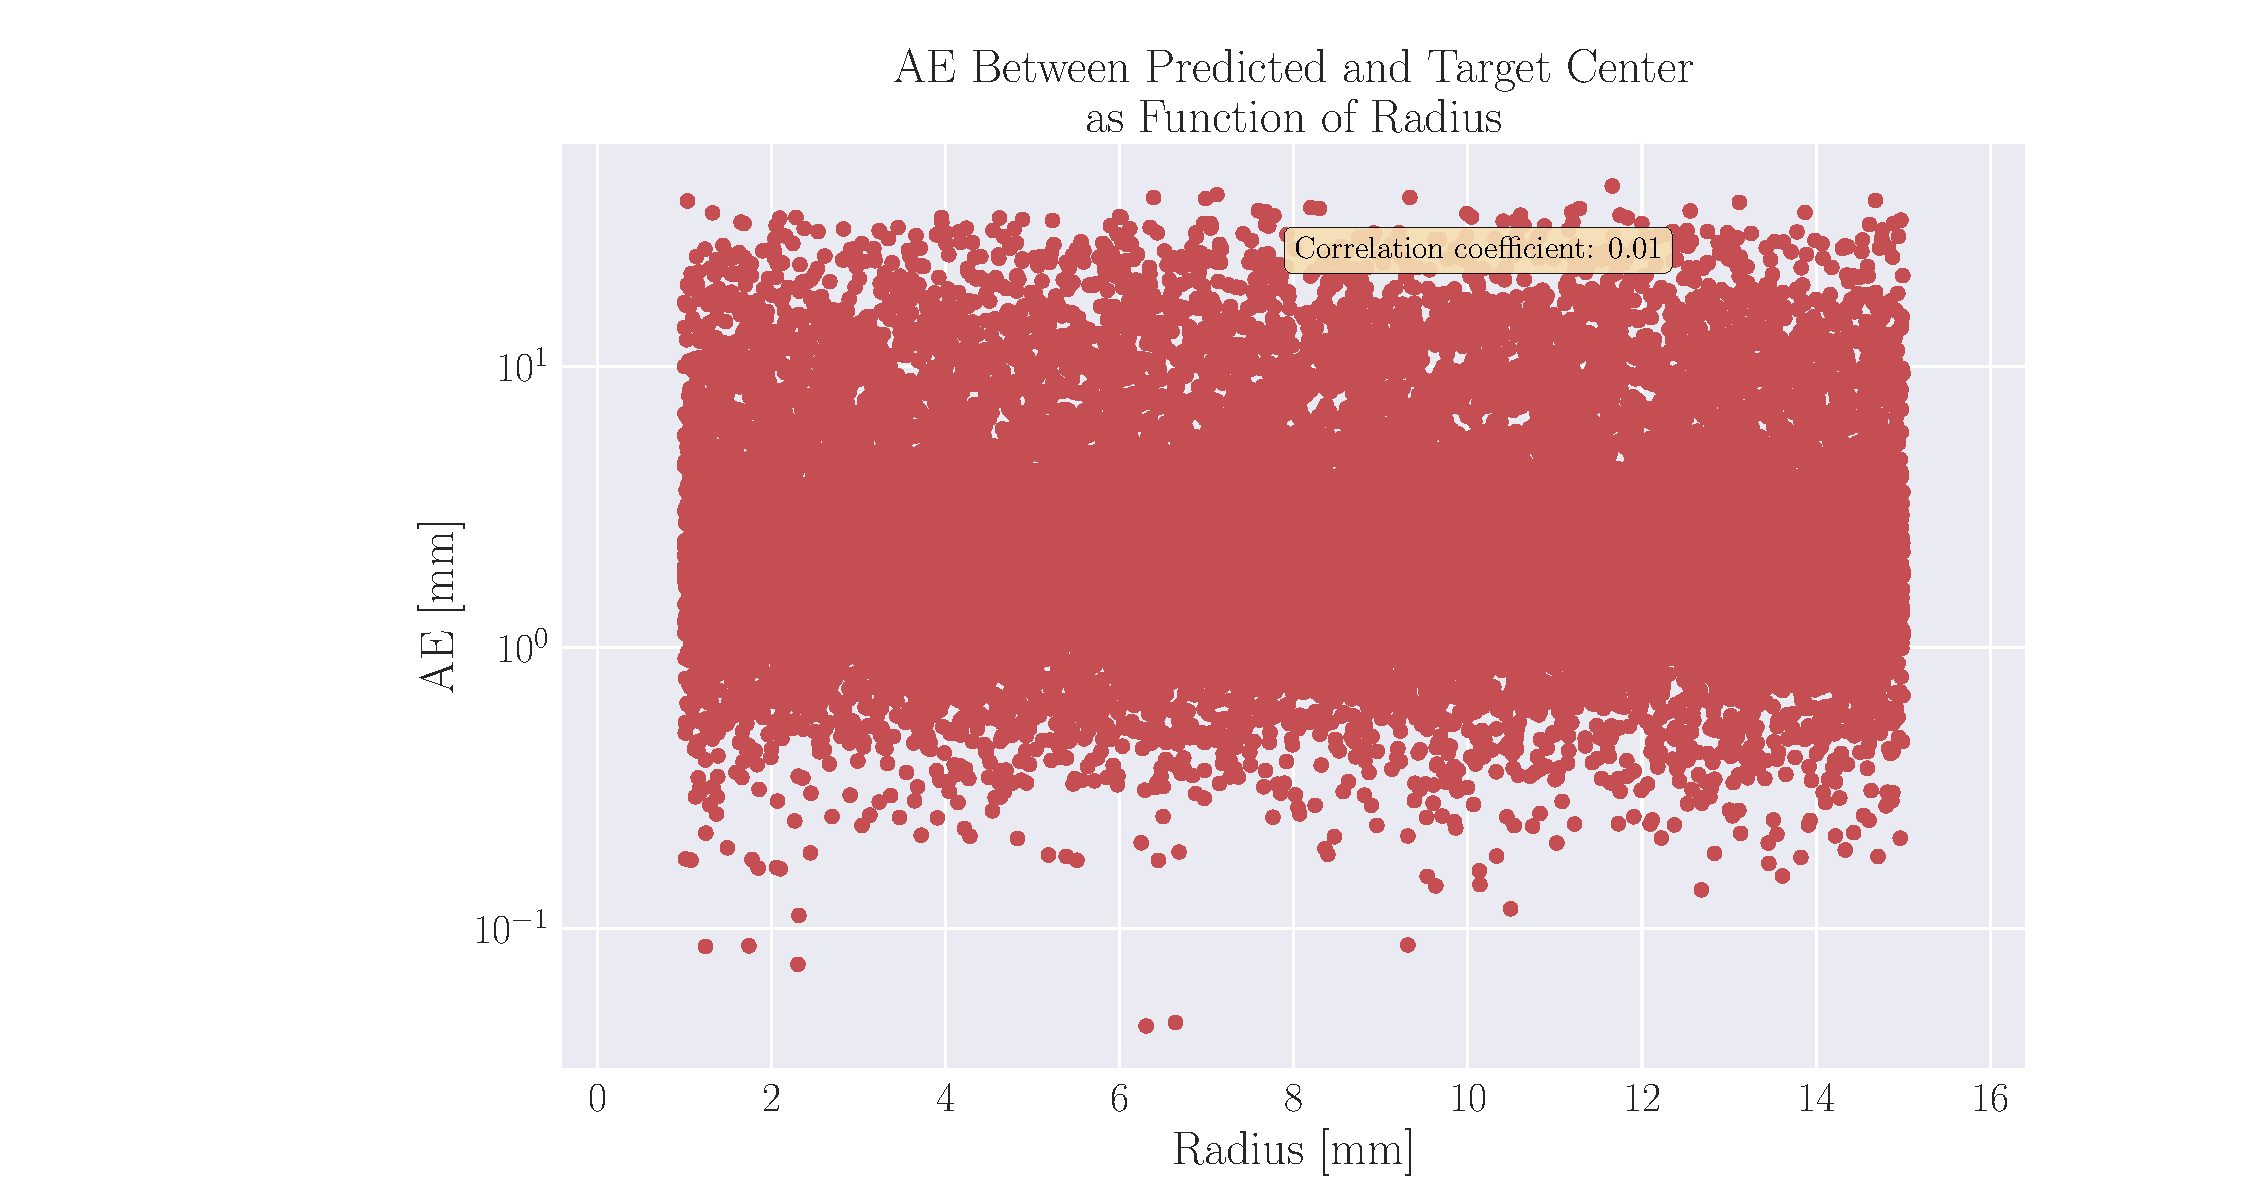
\includegraphics[width=12cm]{figures/mae_area.pdf}
  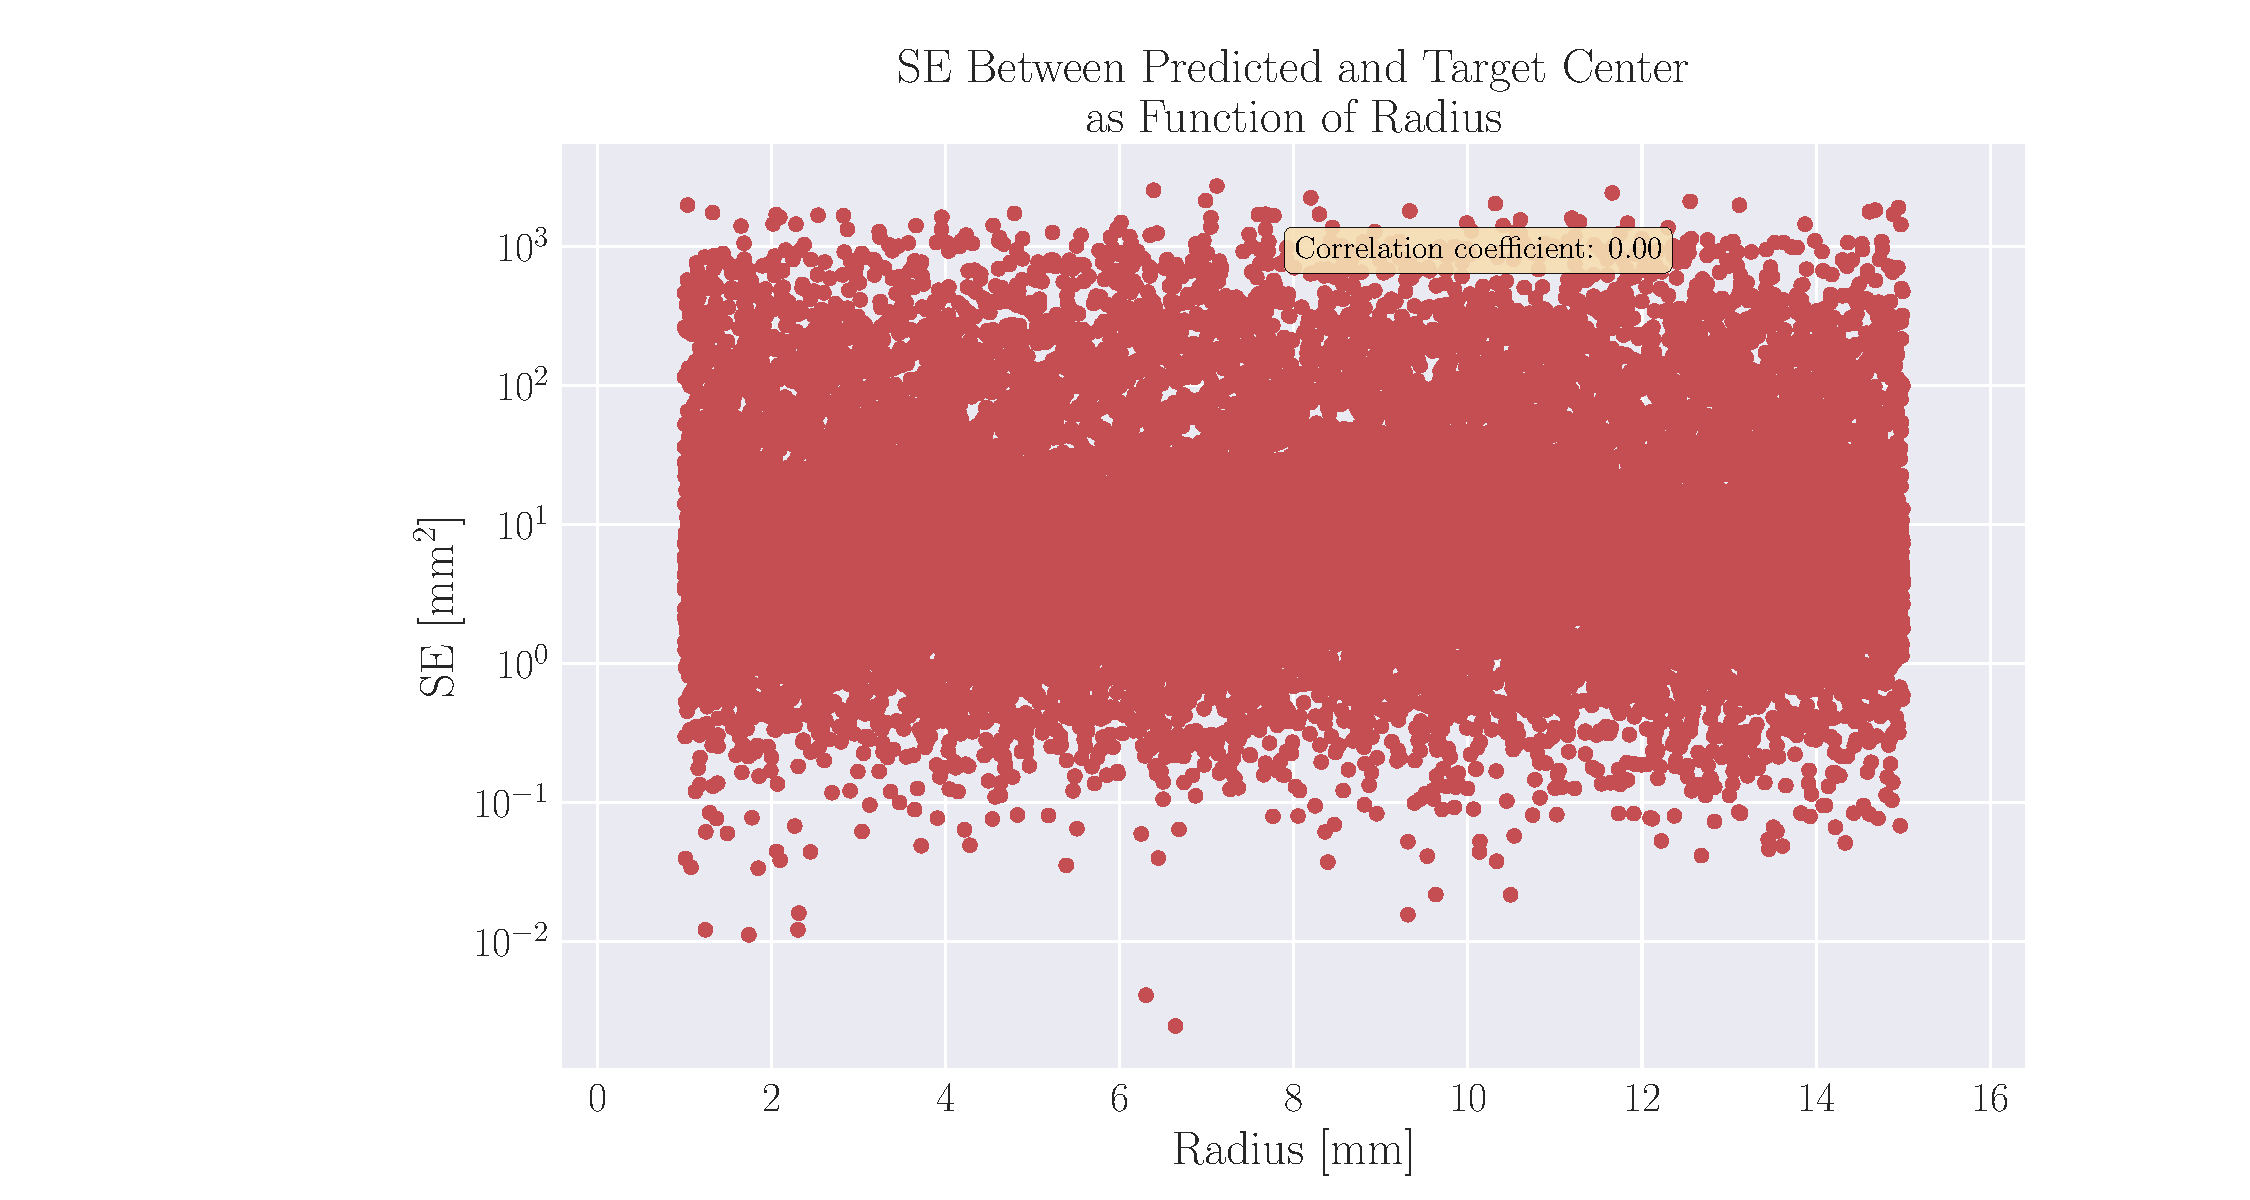
\includegraphics[width=12cm]{figures/mse_area.pdf}
  \caption{\textbf{Dipole Population:}
  Scatter plot of Mean Absolute Error and Mean Squared Error computed between predicted and target center values, as function of the radius of the dipole populations.}
  \label{fig:area_errors}
\end{figure}


\end{document}


\printbibliography

\backmatter


\end{document}